% Practice list --- every topic of the course (Aulas 1-9), weighted toward the Prova 01 error clusters
% (Prova/prova-01-error-analysis.md). Blocks 1-5: Kurlat caps 1-7; blocks 6-9: Kurlat caps 9-11 + Benigno (2015).
% \solucoesfalse -> blank list ; \solucoestrue -> answer key + rubric.
% Compile: pdflatex (2x) with a per-job jobname; check: pdffonts (all Type 1).
% Every result: python practice-all-topics-check-a.py && python practice-all-topics-check-b.py
\documentclass[11pt,a4paper]{article}
% Shared preamble of the practice lists (practice-L*.tex), adapted from lista-exam.tex.
% Each list sets \solucoesfalse / \solucoestrue and \listatema right after \input{practice-preamble}.
\usepackage[utf8]{inputenc}
\usepackage[T1]{fontenc}
\usepackage{lmodern}   % Type 1 vector fonts (replaces PK bitmaps)
\usepackage{cmap}      % ToUnicode CMap -> copyable text and accents
\usepackage[english]{babel}
\usepackage{amsmath,amssymb,amsfonts}
\usepackage[a4paper,margin=2.2cm]{geometry}
\usepackage{enumitem}
\usepackage{fancyhdr}
\usepackage{comment}
% One cut file per job, so builds running side by side cannot swap each other's solutions.
\def\DefaultCutFileName{\def\CommentCutFile{\jobname.cut}}
\usepackage{xcolor}
\usepackage{microtype}
\usepackage{booktabs}
\usepackage{tikz}
\usepackage{pgfplots}
\pgfplotsset{compat=1.16}

\newif\ifsolucoes
\newcommand{\disciplina}{Macroeconomics I --- MPE Insper}
\newcommand{\espacoresol}{4.5cm}   % height of the answer space in the blank list
% The sol environment must be decided after the list sets its toggle.
\AtBeginDocument{\ifsolucoes\includecomment{sol}\else\excludecomment{sol}\fi}

\pagestyle{fancy}\fancyhf{}
\lhead{\footnotesize\disciplina}
\rhead{\footnotesize Practice list\ifsolucoes{} --- Solutions and rubric\fi}
\cfoot{\footnotesize\thepage}
\renewcommand{\headrulewidth}{0.3pt}
\setlength{\headheight}{14pt}
\setlist{topsep=2pt,itemsep=2pt}
\newcounter{questao}

\newcommand{\bloco}[3]{\par\bigskip\noindent
  {\large\bfseries\color{blue!55!black}Block #1 --- #2}\par\noindent\hfill\textit{(#3)}\par
  \noindent\rule{\linewidth}{0.3pt}\smallskip}
\newcommand{\questao}[1]{\par\refstepcounter{questao}\medskip\noindent
  \textbf{Question \thequestao.}~#1\par}
\newenvironment{alternativas}{\begin{enumerate}[label=\Alph*.,leftmargin=2.2em,topsep=1pt]}{\end{enumerate}}
\newcommand{\gabarito}[1]{\ifsolucoes\par\noindent\textbf{Answer:}~#1\fi}
\newcommand{\resolespaco}{\ifsolucoes\else\par\textit{Solution:}\vspace{\espacoresol}\par\fi}
\newcommand{\passo}[2]{\par\smallskip\noindent\textbf{Step --- #1.}~#2}
\newcommand{\intuicao}[1]{\par\smallskip\noindent\textit{Economic intuition.}~#1}
\newcommand{\refbib}[1]{\par\smallskip\noindent{\footnotesize\color{black!60}\textbf{Ref:} #1}}
\newcommand{\rubrica}[1]{\par\smallskip\noindent\textbf{Grading rubric.}\begin{itemize}[leftmargin=1.4em,topsep=1pt]#1\end{itemize}}

\newcommand{\cabecalho}{%
\begin{center}
  {\Large\bfseries \disciplina}\\[2pt]
  {\large Practice list: \listatema}\ifsolucoes\\[2pt]\textit{Solutions and grading rubric}\fi
\end{center}
\vspace{2pt}
{\footnotesize\noindent\textbf{Instructions.} Multiple choice: mark the single correct option (no
penalty for wrong answers). \emph{True/False}: every 2 wrong items cancel 1 right one
(score $=\max\{0,\text{right}-\text{wrong}/2\}\times$ item value); blank items do not count.
Discursive questions: show every step. Parameters are symbols with the stated admissible
ranges; answers are closed forms, conditions, signs and limits.\par}}

\newenvironment{notacao}{\par\smallskip\noindent\textbf{Notation.}\begin{itemize}[leftmargin=1.4em,topsep=1pt,itemsep=0pt]\small}{\end{itemize}}
\allowdisplaybreaks
\usepackage{needspace}
\solucoestrue                  % <<<< \solucoestrue for the ANSWER KEY
\newcommand{\listatema}{Every topic of the course (Aulas 1--9)}
\renewcommand{\espacoresol}{5.5cm}

\begin{document}
\cabecalho

% =============================================================================
% Block 1 --- Aula 1: measurement (GDP by three approaches, price indices, PPP, beyond GDP).
% Weighted toward Prova 01 error cluster 1 (every approach computed, and they must agree).
\bloco{1}{Measuring aggregates: GDP, price indices, PPP, beyond GDP}{Aula 1 \,\textbullet\, Kurlat chs.~1--2 \,\textbullet\, 10 points}

\questao{(4 points) \textit{Source: Kurlat, P. (2020), \emph{A Course in Modern Macroeconomics}, Exercise 1.3 ``Chained GDP'',
pp.~28--29 --- statement reproduced verbatim, all items (a)--(c).}}

\noindent The country of Fructus produces Apples, Bananas and Cherries. Its production statistics are given below:
\begin{center}\small
\begin{tabular}{@{}l*{6}{r}@{}}
\toprule
 & \multicolumn{2}{c}{\textbf{Apples}} & \multicolumn{2}{c}{\textbf{Bananas}} & \multicolumn{2}{c}{\textbf{Cherries}} \\
\cmidrule(lr){2-3}\cmidrule(lr){4-5}\cmidrule(l){6-7}
 & quantity & price & quantity & price & quantity & price \\
\midrule
2000 & 100 & 40 & 50 & 30 & 200 & 20 \\
2001 & 103 & 39 & 47 & 35 & 206 & 20 \\
2002 & 107 & 39 & 47 & 38 & 213 & 19 \\
2003 & 109 & 39 & 45 & 38 & 215 & 18 \\
2004 & 112 & 40 & 46 & 41 & 224 & 18 \\
2005 & 112 & 39 & 46 & 39 & 227 & 17 \\
2006 & 114 & 40 & 47 & 36 & 237 & 16 \\
2007 & 115 & 40 & 46 & 42 & 249 & 16 \\
2008 & 119 & 40 & 43 & 44 & 255 & 16 \\
2009 & 118 & 42 & 40 & 46 & 262 & 15 \\
2010 & 116 & 43 & 41 & 44 & 268 & 15 \\
2011 & 118 & 42 & 40 & 50 & 280 & 15 \\
2012 & 117 & 42 & 41 & 50 & 289 & 15 \\
2013 & 119 & 43 & 40 & 53 & 290 & 14 \\
2014 & 120 & 44 & 40 & 56 & 297 & 13 \\
2015 & 125 & 45 & 41 & 59 & 308 & 13 \\
2016 & 128 & 45 & 38 & 66 & 320 & 13 \\
2017 & 129 & 46 & 38 & 61 & 330 & 13 \\
2018 & 131 & 47 & 37 & 64 & 344 & 13 \\
2019 & 136 & 47 & 37 & 61 & 353 & 13 \\
2020 & 143 & 47 & 34 & 61 & 361 & 12 \\
\bottomrule
\end{tabular}
\end{center}
\noindent(you can download them as an Excel spreadsheet from the book website)
\begin{enumerate}[label=(\alph*),leftmargin=2.2em,topsep=2pt,itemsep=1pt]
\item Compute a real GDP series at year-2000 prices using base year prices and using the chained method.
\item Plot both series and comment on any differences.
\item What was the average growth rate according to each method?
\end{enumerate}
\noindent\textit{Added to the book's items (not in the book):} use the chained method of Kurlat \S1.2; show the 2000--2001 link in full,
describe the plot of (b) in words, and report both series for 2000, 2005, 2010, 2015 and 2020 and the average growth rates.
\resolespaco
\begin{sol}
\begin{notacao}
\item $i\in\{A,B,C\}$: the three goods of the table (B are bananas, C cherries).
\item $p_{i,t}>0$, $q_{i,t}>0$: price and quantity of good $i$ in year $t\in\{2000,\dots,2020\}$.
\item $Y_t$: real GDP at constant 2000 prices. $Y^{ch}_t$: chained real GDP, expressed in 2000 prices.
\item $g^I_t$, $g^F_t$: growth from $t-1$ to $t$ valued at initial ($t-1$) and at final ($t$) prices. $g_t$: chained growth.
\item $\bar g$: average annual growth rate over 2000--2020.
\end{notacao}
\passo{base-year prices}{Real GDP at constant prices values each year's quantities at the 2000 prices,
$(p_A,p_B,p_C)_{2000}=(40,30,20)$:}
\begin{equation}
Y_t=\textstyle\sum_i p_{i,2000}\,q_{i,t}. \label{b1q1:base}
\end{equation}
Using \eqref{b1q1:base} for 2000 and 2001:
\begin{align*}
Y_{2000}&=40\times100+30\times50+20\times200\\
&=4{,}000+1{,}500+4{,}000=9{,}500,\\
Y_{2001}&=40\times103+30\times47+20\times206\\
&=4{,}120+1{,}410+4{,}120=9{,}650.
\end{align*}
\passo{the 2001 chain link}{Kurlat's chained method measures each year's growth at both years' prices and
takes the geometric average:}
\begin{align}
1+g^I_t&=\frac{\sum_i p_{i,t-1}\,q_{i,t}}{\sum_i p_{i,t-1}\,q_{i,t-1}}, \label{b1q1:gI}\\
1+g^F_t&=\frac{\sum_i p_{i,t}\,q_{i,t}}{\sum_i p_{i,t}\,q_{i,t-1}}, \label{b1q1:gF}\\
1+g_t&=\big[(1+g^I_t)(1+g^F_t)\big]^{1/2}, \label{b1q1:g}\\
Y^{ch}_t&=Y^{ch}_{t-1}\,(1+g_t),\qquad Y^{ch}_{2000}=Y_{2000}. \label{b1q1:chain}
\end{align}
For 2001 the initial prices are the 2000 prices, so \eqref{b1q1:gI} is the ratio of the two sums of the previous step:
\[
1+g^I_{2001}=\frac{9{,}650}{9{,}500}=1.01579 .
\]
At the 2001 prices, $(39,35,20)$:
\begin{align*}
\textstyle\sum_i p_{i,2001}\,q_{i,2001}&=39\times103+35\times47+20\times206\\
&=4{,}017+1{,}645+4{,}120=9{,}782,\\
\textstyle\sum_i p_{i,2001}\,q_{i,2000}&=39\times100+35\times50+20\times200\\
&=3{,}900+1{,}750+4{,}000=9{,}650.
\end{align*}
Substituting these into \eqref{b1q1:gF}:
\[
1+g^F_{2001}=\frac{9{,}782}{9{,}650}=1.01368 .
\]
Using \eqref{b1q1:g}:
\[
1+g_{2001}=(1.01579\times1.01368)^{1/2}=1.01473 ,
\]
a chained growth of $1.473\%$. Using \eqref{b1q1:chain}:
\begin{align*}
Y^{ch}_{2001}&=9{,}500\times(1+g_{2001})\\
&=9{,}500\times(1.014734)\\
&=9{,}639.97 .
\end{align*}
Repeating \eqref{b1q1:gI}--\eqref{b1q1:chain} every year:
\begin{center}\small
\begin{tabular}{@{}lccccc@{}}
\toprule
 & 2000 & 2005 & 2010 & 2015 & 2020 \\
\midrule
At 2000 prices & 9{,}500 & 10{,}400 & 11{,}230 & 12{,}390 & 13{,}960 \\
Chained (2000 prices) & 9{,}500 & 10{,}341.8 & 10{,}950.0 & 11{,}922.8 & 12{,}976.2 \\
\bottomrule
\end{tabular}
\end{center}
\passo{(b) the gap}{The fixed-price series grows faster and the gap widens every year. Cherries expand most ($200\to361$) while
their relative price falls ($20\to12$); bananas shrink ($50\to34$) while theirs rises ($30\to61$). The fixed 2000 prices in
\eqref{b1q1:base} keep weighting cherries at their old, high price, so they overstate growth; \eqref{b1q1:gI}--\eqref{b1q1:gF}
update the weights every year.}
\passo{(c) average growth}{The average annual rate compounds over the 20 years:}
\begin{equation}
1+\bar g=\Big(\frac{Y_{2020}}{Y_{2000}}\Big)^{1/20}. \label{b1q1:avg}
\end{equation}
Applying \eqref{b1q1:avg} to each series of the table:
\begin{align*}
\text{at 2000 prices:}\quad 1+\bar g&=(13{,}960/9{,}500)^{1/20}=1.0194,\\
\text{chained:}\quad 1+\bar g&=(12{,}976.2/9{,}500)^{1/20}=1.0157,
\end{align*}
that is, $1.94\%$ and $1.57\%$ a year.
\intuicao{A base year far in the past weights each good by a relative price that no longer holds; when the goods that grow most are the
ones getting cheaper, that weighting inflates measured real growth.}
\refbib{Kurlat (2020), ch.~1, \S1.2, ``Alternative 3: chained prices'' (pp.~22--24); Exercise~1.5 (p.~29) asks why expanding sectors
tend to get cheaper. The book prints no answer; every figure is recomputed in the check script.}
\rubrica{
\item (a) base-year series 1 pt, chained series with the 2001 link shown 1.5 pts; (b) 0.75 pt; (c) 0.75 pt.
\item Chained growth computed as an arithmetic average of $g^I$ and $g^F$: $-0.25$ pt (the numbers barely change, the method does).
Average growth taken as the arithmetic mean of annual rates: $-0.25$ pt. Series at current prices called ``real'': max.\ 1 pt.
}
\end{sol}

% -----------------------------------------------------------------------------
\questao{(5 points) Discursive. \emph{Three approaches $\times$ price indices $\times$ beyond GDP.} An illustrative Brazilian
economy (BRL billion, 2025) has four producers.
\begin{itemize}[leftmargin=1.4em]
\item Agro firm F grows soybeans with no intermediate inputs. It sells 300 to the food processor P, exports 200 and pays wages of 250.
\item P buys the 300 of soybeans, imports packaging for 100 and buys 40 of online advertising from N. It produces 700 of food:
households buy 650 and 50 stays unsold in P's warehouse. P pays wages of 180.
\item Platform N gives households a free app financed by advertising; its only sale is the 40 of ads to P, and it pays 30 to the app
staff. It also pays 60 in wages to programmers who write software that N will use in its own operations for ten years.
\item The government pays 120 in wages to public school teachers and 80 in Bolsa Fam\'ilia transfers, financed by taxes.
\end{itemize}
Each firm's profit is its revenue plus any output added to its own stocks, minus wages and intermediate inputs.}

\textbf{a)} (2 points) Compute 2025 GDP by the production, income and expenditure approaches, and show that they agree.
\resolespaco
\begin{sol}
\begin{notacao}
\item $j\in\{F,P,N,\text{Gov}\}$: the agro firm, the food processor, the platform and the government (BRL billion, 2025).
\item $VA_j$: value added of producer $j$. $W_j\ge0$: wages it pays. $\Pi_j$: its profit (statement's definition).
\item $C$, $I$, $G$, $X$, $M$: household consumption, investment (fixed capital plus inventories), government purchases
of goods and services, exports and imports.
\end{notacao}
\passo{the four identities used below}{GDP is the value of final goods and services produced; the three approaches must
agree:}
\begin{align}
\text{GDP}&=\textstyle\sum_j VA_j, \label{b1q2:gdpva}\\
VA_j&=\text{gross output}_j-\text{intermediate inputs}_j, \label{b1q2:va}\\
\text{GDP}&=\textstyle\sum_j W_j+\sum_j\Pi_j, \label{b1q2:inc}\\
\text{GDP}&=C+I+G+X-M. \label{b1q2:exp}
\end{align}
The government sells nothing, so its output is valued at cost: its value added is its wage bill.
\passo{production (value added)}{P's gross output is its sales plus the food added to its stocks:
$650+50=700$. Own-account software is valued at cost, 60. Using \eqref{b1q2:va}:}
\begin{align*}
VA_F&=500-0=500,\\
VA_P&=700-300-100-40=260,\\
VA_N&=(40+60)-0=100,\\
VA_{\text{Gov}}&=120.
\end{align*}
Summing with \eqref{b1q2:gdpva}:
\[
\text{GDP}=500+260+100+120=980 .
\]
\passo{income}{Wages, with N paying the app staff and the programmers:}
\[
\textstyle\sum_j W_j=250+180+(30+60)+120=640 .
\]
Profits, by the statement's definition (revenue plus own stocks, minus wages and inputs):
\begin{align*}
\Pi_F&=500-250=250,\\
\Pi_P&=700-300-100-40-180=80,\\
\Pi_N&=100-90=10,
\end{align*}
a total of $340$. Using \eqref{b1q2:inc}:
\[
\text{GDP}=640+340=980 .
\]
\passo{expenditure}{$C=650$ (the app is free: no transaction). $I$ is inventory plus software, which is gross fixed capital
formation: $I=50+60=110$. $G=120$ (the transfer of 80 buys no good or service). $X=200$, $M=100$. Using \eqref{b1q2:exp}:}
\[
\text{GDP}=650+110+120+200-100=980 .
\]
\passo{traps}{Summing gross outputs, $500+700+100+120=1{,}420$, double counts the soybeans and the ads, which P uses up;
\eqref{b1q2:va} nets them out.}
\refbib{Kurlat (2020), ch.~1, \S1.1 (p.~15); Prova~01, Q1(b)--(c) (\texttt{Prova/}\allowbreak\texttt{prova-01-error-analysis.md}).}
\rubrica{
\item 0.7 pt per approach (2 pts in total with agreement). Software placed in $C$, or the transfer in $G$: max.\ 1 pt in the item.
}
\end{sol}

\textbf{b)} (1.5 points) Give the number and the reason in each case. (i) GDP if N books the software as a current expense.
(ii) GDP a student obtains by counting Bolsa Fam\'ilia in $G$. (iii) Gross national income if 30 of F's profit belongs to a foreign
shareholder. (iv) What part of the app's value to households GDP records, and how a welfare measure such as Jones--Klenow's would treat it.
\resolespaco
\begin{sol}
\begin{notacao}
\item Symbols as in (a). GNI: gross national income, the factor income of residents.
\end{notacao}
\passo{(i)}{Expensed, the software is an intermediate input of N. Using \eqref{b1q2:va} and then \eqref{b1q2:exp}, with
$I=50$:}
\begin{align*}
VA_N&=100-60=40,\\
\text{GDP}&=650+50+120+200-100=920 .
\end{align*}
National accounts capitalise own-account software as investment in intellectual property, because it is a durable
productive asset; then GDP $=980$, as in (a).
\passo{(ii)}{$980+80=1{,}060$ is wrong: a transfer moves income from taxpayers to families and pays for no current production,
so it is not in $G$ in \eqref{b1q2:exp}. It enters $C$ only when the families spend it, and that spending is already in the 650.}
\passo{(iii)}{GDP is territorial; GNI counts the income of residents:}
\begin{equation}
\text{GNI}=\text{GDP}-\text{factor income paid abroad}+\text{factor income received from abroad}. \label{b1q2:gni}
\end{equation}
Using \eqref{b1q2:gni}, with nothing received from abroad:
\[
\text{GNI}=980-30+0=950 .
\]
\passo{(iv)}{GDP records only the 40 of ads, as an intermediate input of P that is already inside the price of food. The service
households get at price zero is not a market transaction, so its value is missing from GDP. A consumption-based welfare
measure (Kurlat ch.~2) would count it only if it were valued, e.g.\ by households' willingness to pay or time spent.}
\refbib{Kurlat (2020), ch.~1, \S1.1 and ch.~2, \S2.1--2.2 (pp.~31--33).}
\rubrica{\item 0.375 pt per sub-case, number and reason. Number without the reason: half.}
\end{sol}

\textbf{c)} (1.5 points) In 2026 every quantity repeats, while prices change: food $+10\%$, soybeans $+20\%$ (domestic and
export price), imported packaging $+50\%$, teachers' wages $+5\%$; ads and software unchanged. Compute nominal GDP in 2026, real GDP at
2025 prices and the inflation rate of the GDP deflator. Compare it with a consumer price index (IPCA-type, Laspeyres) built on the
household basket, and explain the gap.
\resolespaco
\begin{sol}
\begin{notacao}
\item Symbols as in (a); subscripts 2025 and 2026 date a value. Quantities $q$ are the same in both years.
\item $P^D_t$: GDP deflator, nominal over real GDP, with $P^D_{2025}=1$. $\pi^D$: its inflation rate.
\item $\text{CPI}_t$: Laspeyres consumer price index on the 2025 household basket $q^H_{2025}$, with $\text{CPI}_{2025}=1$.
\end{notacao}
\passo{nominal GDP}{Each 2025 component of \eqref{b1q2:exp} is multiplied by its price change (software is unchanged):}
\begin{align*}
C&=650\times1.1=715,\\
I&=50\times1.1+60=115,\\
G&=120\times1.05=126,\\
X&=200\times1.2=240,\\
M&=100\times1.5=150.
\end{align*}
Using \eqref{b1q2:exp}:
\begin{equation}
\text{GDP}^{\text{nom}}_{2026}=715+115+126+240-150=1{,}046. \label{b1q2:nom}
\end{equation}
Production check with \eqref{b1q2:va}: F sells $300\times1.2=360$ at home and exports $240$; P's output is $715+55=770$:
\begin{align*}
VA_F&=360+240=600,\\
VA_P&=770-360-150-40=220,\\
VA_N&=100,\qquad VA_{\text{Gov}}=126,
\end{align*}
and \eqref{b1q2:gdpva} gives $600+220+100+126=1{,}046$.
\passo{real GDP and deflator}{At 2025 prices the 2026 quantities give the 2025 value, since nothing moved:}
\begin{equation}
\text{GDP}^{\text{real}}_{2026}=980. \label{b1q2:real}
\end{equation}
The deflator is the ratio of \eqref{b1q2:nom} to \eqref{b1q2:real}:
\[
P^D_{2026}=\frac{1{,}046}{980}=1.0673,\qquad \pi^D=6.73\% .
\]
Real growth is zero, so all of the $6.73\%$ nominal growth is price.
\passo{CPI}{Households buy only food (the app costs zero; the transfer is not a good), so the Laspeyres index is}
\[
\text{CPI}_{2026}=\frac{\sum_i p_{i,2026}\,q^H_{i,2025}}{\sum_i p_{i,2025}\,q^H_{i,2025}}=\frac{650\times1.1}{650}=1.10,
\]
a rise of $10\%$.
\passo{the gap}{The deflator prices domestic production. Splitting the rise from \eqref{b1q2:real} to \eqref{b1q2:nom} by item:
food $700\times0.10=70$, teachers $120\times0.05=6$, exports $200\times0.20=40$, imports $-100\times0.50=-50$
(the soybeans sold to P cancel between F and P):}
\begin{align*}
\text{GDP}^{\text{nom}}_{2026}-\text{GDP}^{\text{real}}_{2026}&=70+6+40-50=66,\\
\pi^D&=66/980=6.73\% .
\end{align*}
Dearer imports \emph{lower} the deflator, because $M$ is subtracted, and exports raise it. The CPI prices what households
consume, imported goods included, with fixed base-year weights.
\refbib{Kurlat (2020), ch.~1, \S1.2 (p.~22).}
\rubrica{
\item Nominal GDP 0.5; deflator 0.5; CPI and the gap 0.5. Imports added rather than subtracted: max.\ 0.5 pt. Arithmetic slip with the right
method: $-0.25$ pt.
}
\end{sol}

% -----------------------------------------------------------------------------
\questao{(1 point) Multiple choice. Brazil's GDP per capita is BRL~60{,}000 (illustrative); the market exchange rate is 5.0 BRL per USD and
the Penn World Table PPP conversion factor is 2.5 BRL per USD; US GDP per capita is USD~85{,}000. Which statement is correct?}
\begin{alternativas}
\item At PPP Brazil's GDP per capita is USD~12{,}000, about 14\% of the US level, since PPP strips out the cheaper Brazilian tradables.
\item At PPP it is USD~24{,}000, about 28\% of the US level, because tradable goods are cheaper in Brazil while the real is undervalued.
\item At PPP it is USD~24{,}000, about 28\% of the US level, because non-tradable services are cheaper in Brazil, so a real buys more there.
\item At PPP it is USD~150{,}000, about 176\% of the US level, because PPP converts reais at the price of a common basket of goods.
\item At market rates it is USD~24{,}000 and at PPP USD~12{,}000, so the market rate overstates Brazilian living standards.
\end{alternativas}
\gabarito{C}
\begin{sol}
\begin{notacao}
\item $y=60{,}000$: GDP per capita in BRL; $e$: a conversion rate in BRL per USD (market $5.0$, PPP $2.5$); $y^{US}=85{,}000$ USD.
\end{notacao}
\passo{numbers}{A value in BRL is converted to USD by dividing by the rate:}
\begin{equation}
y^{USD}=\frac{y}{e}. \label{b1q3:conv}
\end{equation}
Using \eqref{b1q3:conv} at each rate, then dividing by $y^{US}$:
\begin{align*}
\text{market:}\quad y^{USD}&=60{,}000/5.0=12{,}000, & 12{,}000/85{,}000&=14.1\%,\\
\text{PPP:}\quad y^{USD}&=60{,}000/2.5=24{,}000, & 24{,}000/85{,}000&=28.2\%.
\end{align*}
\passo{reason}{The PPP factor is below the market rate because non-tradables (haircuts, rents, services) are cheaper in a
lower-productivity country (Balassa--Samuelson); tradables roughly obey the law of one price. A uses the market number with the wrong
label; B has the right number with the tradables story; D multiplies by the PPP factor ($60{,}000\times2.5$) and keeps a wrong reason
(two mistakes); E swaps the two conversions.}
\refbib{Kurlat (2020), ch.~1, \S1.2 (PPP comparisons, p.~22); Jones (2020), ch.~2.}
\end{sol}

% =============================================================================
% Block 2 --- Aula 2: Solow mechanics (per worker, no technological progress).
% Weighted toward Prova 01 error cluster 2 (carry the exponent; level versus growth effects).
\bloco{2}{The Solow model: mechanics}{Aula 2 \,\textbullet\, Kurlat ch.~3, \S4.1--4.2 \,\textbullet\, 10 points}

\questao{(4 points) \textit{Source: Kurlat, P. (2020), \emph{A Course in Modern Macroeconomics}, Exercise 4.2 ``The Black Death'',
pp.~72--73 --- statement reproduced verbatim, all items (a)--(d).}}

\noindent In the middle of the 14th century, a plague killed about a third of the population of Europe. Assume that the economy of Europe
was well described by the Solow model. How would the following variables change in response to the Black Death in the short run
(i.e.\ immediately)?
\begin{enumerate}[label=(\alph*),leftmargin=2.2em,topsep=2pt,itemsep=1pt]
\item GDP,
\item GDP per capita,
\item wages,
\item interest rates.
\end{enumerate}
\noindent\textit{Added parts (not in the book):} use $Y=AK^{\alpha}L^{1-\alpha}$; give each change as a factor and, with $\alpha=1/3$, as a
percentage. Then add one line per variable on the long run, with $s$, $n$, $\delta$ and $A$ unchanged.
\resolespaco
\begin{sol}
\begin{notacao}
\item $Y$, $K$, $L$: output, capital and population (= labour force). $A>0$: productivity. $\alpha\in(0,1)$: capital share, here $1/3$.
\item $k\equiv K/L$, $y\equiv Y/L$: capital and output per capita. $w$: real wage. $r^K$: rental rate of capital.
$r$: real interest rate. $\delta\in(0,1)$: depreciation. $s$, $n$: saving rate and population growth.
\item A prime marks a value just after the plague; $k^*$: the steady-state capital per capita.
\end{notacao}
\passo{model and prices}{The statement's technology, and its per-capita form (divide by $L$):}
\begin{align}
Y&=AK^{\alpha}L^{1-\alpha}, \label{b2q4:Y}\\
y&=Ak^{\alpha}. \label{b2q4:y}
\end{align}
Competitive factor prices are the marginal products of \eqref{b2q4:Y}:
\begin{align}
w&=\frac{\partial Y}{\partial L}=(1-\alpha)Ak^{\alpha}, \label{b2q4:w}\\
r^K&=\frac{\partial Y}{\partial K}=\alpha Ak^{\alpha-1},\qquad r=r^K-\delta. \label{b2q4:rK}
\end{align}
\passo{the shock}{On impact a third of the population dies and capital does not:}
\begin{equation}
\frac{L'}{L}=\frac23,\qquad \frac{K'}{K}=1,\qquad\text{so}\qquad \frac{k'}{k}=\frac32. \label{b2q4:shock}
\end{equation}
\passo{(a) GDP}{Divide \eqref{b2q4:Y} after the shock by \eqref{b2q4:Y} before, and use \eqref{b2q4:shock}:}
\begin{align*}
\frac{Y'}{Y}&=\frac{A(K')^{\alpha}(L')^{1-\alpha}}{AK^{\alpha}L^{1-\alpha}}\\
&=\Big(\frac{K'}{K}\Big)^{\alpha}\Big(\frac{L'}{L}\Big)^{1-\alpha}\\
&=(1)^{\alpha}\Big(\frac23\Big)^{1-\alpha}\\
&=\Big(\frac23\Big)^{2/3}=0.763 .
\end{align*}
GDP falls about $24\%$, less than the third of the population, because labour has diminishing returns.
\passo{(b) GDP per capita}{Using \eqref{b2q4:y} and \eqref{b2q4:shock}:}
\begin{align*}
\frac{y'}{y}&=\frac{A(k')^{\alpha}}{Ak^{\alpha}}\\
&=\Big(\frac{k'}{k}\Big)^{\alpha}=\Big(\frac32\Big)^{1/3}=1.145 .
\end{align*}
It \emph{rises} about $14.5\%$.
\passo{(c) wages}{Using \eqref{b2q4:w} and \eqref{b2q4:shock}:}
\begin{align*}
\frac{w'}{w}&=\frac{(1-\alpha)A(k')^{\alpha}}{(1-\alpha)Ak^{\alpha}}\\
&=\Big(\frac{k'}{k}\Big)^{\alpha}=\Big(\frac32\Big)^{1/3}=1.145 ,
\end{align*}
a rise of $14.5\%$.
\passo{(d) interest rate}{Using \eqref{b2q4:rK} and \eqref{b2q4:shock}:}
\begin{align*}
\frac{r^{K\prime}}{r^K}&=\frac{\alpha A(k')^{\alpha-1}}{\alpha Ak^{\alpha-1}}\\
&=\Big(\frac{k'}{k}\Big)^{\alpha-1}=\Big(\frac32\Big)^{-2/3}=0.763 .
\end{align*}
The rental rate falls about $24\%$, and by \eqref{b2q4:rK} $r=r^K-\delta$ falls by the same absolute amount.
\passo{long run}{$k'$ is above $k^*$, so saving per capita falls short of break-even investment, $sA(k')^{\alpha}<(n+\delta)k'$,
and $k$ falls back to the unchanged $k^*$. By \eqref{b2q4:y}--\eqref{b2q4:rK}, $y$, $w$ and $r$ return to their old values. $K$ and $Y$
converge to $\frac23$ of the path they would have followed: the population loss is permanent, its per-capita gain is
transitory.}
\intuicao{Labour became scarce relative to capital, so its marginal product rose and capital's fell; the survivors were richer
only until capital per worker depreciated back to the steady state.}
\refbib{Kurlat (2020), \S4.2 and \S4.4 (pp.~57, 63). The project's worked solution (Problem 4.2, folder
\texttt{Resolucao}) agrees on (a)--(c) but prints $0.874$ for (d), which is $(3/2)^{-1/3}$; the correct factor is $(3/2)^{-2/3}=0.763$.}
\rubrica{
\item 0.75 pt per item (a)--(d) with direction and factor; long run 1 pt. Wrong direction of $y$ or $w$ (thinking in totals): max.\ 0.25 pt in that item.
}
\end{sol}

% -----------------------------------------------------------------------------
\questao{(5 points) Discursive. \emph{Steady state $\times$ saving reform $\times$ convergence.} Per-worker variables throughout
($k=K/L$, $y=Y/L$, $c=C/L$). $Y_t=AK_t^{\alpha}L_t^{1-\alpha}$, $K_{t+1}=(1-\delta)K_t+sY_t$, $L_{t+1}=(1+n)L_t$, no technological
progress. Illustrative calibration for Brazil: $A=1$, $\alpha=1/3$, $s=0.20$, $n=0.02$, $\delta=0.08$.}

\textbf{a)} (2 points) Derive the law of motion of $k_t$ and find $k^*$, $y^*$ and $c^*$ in closed form in $(A,s,n,\delta,\alpha)$, then in
numbers. Use the limit $\alpha\to0$ to check the exponent of $y^*$.
\resolespaco
\begin{sol}
\begin{notacao}
\item $Y_t$, $K_t$, $L_t$: output, capital and workers in period $t$. $A>0$: productivity (constant). $\alpha\in(0,1)$: capital share.
\item $s\in(0,1)$: saving rate. $n\ge0$: labour-force growth. $\delta\in(0,1)$: depreciation.
\item $k_t\equiv K_t/L_t$, $y_t\equiv Y_t/L_t$, $c_t\equiv C_t/L_t$: per-worker capital, output and consumption.
$k^*$, $y^*$, $c^*$: their steady-state values.
\end{notacao}
\passo{the statement's equations}{Numbered here for reference:}
\begin{align}
Y_t&=AK_t^{\alpha}L_t^{1-\alpha}, \label{b2q5:Y}\\
K_{t+1}&=(1-\delta)K_t+sY_t, \label{b2q5:K}\\
L_{t+1}&=(1+n)L_t. \label{b2q5:L}
\end{align}
Dividing \eqref{b2q5:Y} by $L_t$ gives the per-worker technology:
\begin{equation}
y_t=Ak_t^{\alpha}. \label{b2q5:y}
\end{equation}
\passo{law of motion}{Divide \eqref{b2q5:K} by $L_{t+1}$, substitute \eqref{b2q5:Y} for $Y_t$ and \eqref{b2q5:L} for $L_{t+1}$:}
\begin{align}
k_{t+1}&=\frac{K_{t+1}}{L_{t+1}}\nonumber\\
&=\frac{(1-\delta)K_t+sAK_t^{\alpha}L_t^{1-\alpha}}{(1+n)L_t}\nonumber\\
&=\frac{(1-\delta)k_t+sAk_t^{\alpha}}{1+n}. \label{b2q5:lom}
\end{align}
\passo{steady state}{Set $k_{t+1}=k_t=k^*$ in \eqref{b2q5:lom} and multiply by $1+n$:}
\begin{align}
(1+n)k^*&=(1-\delta)k^*+sA(k^*)^{\alpha}\nonumber\\
(n+\delta)k^*&=sA(k^*)^{\alpha} \label{b2q5:be}\\
(k^*)^{1-\alpha}&=\frac{sA}{n+\delta}. \nonumber
\end{align}
Raise both sides to the power $1/(1-\alpha)$:
\begin{equation}
k^*=\Big(\frac{sA}{n+\delta}\Big)^{\frac1{1-\alpha}}. \label{b2q5:kss}
\end{equation}
Substitute \eqref{b2q5:kss} into \eqref{b2q5:y}:
\begin{align}
y^*&=A(k^*)^{\alpha}\nonumber\\
&=A\Big(\Big(\frac{sA}{n+\delta}\Big)^{\frac1{1-\alpha}}\Big)^{\alpha}\nonumber\\
&=A\Big(\frac{sA}{n+\delta}\Big)^{\frac{\alpha}{1-\alpha}}\nonumber\\
&=A^{\frac1{1-\alpha}}\Big(\frac{s}{n+\delta}\Big)^{\frac{\alpha}{1-\alpha}}. \label{b2q5:yss}
\end{align}
Consumption is the output not saved:
\begin{equation}
c^*=(1-s)\,y^*. \label{b2q5:css}
\end{equation}
\passo{numbers}{With $A=1$, $\frac1{1-\alpha}=\frac32$ and $\frac{\alpha}{1-\alpha}=\frac12$, the ratio is $s/(n+\delta)=0.20/0.10=2$.
Using \eqref{b2q5:kss}, \eqref{b2q5:yss} and \eqref{b2q5:css}:}
\begin{align*}
k^*&=\Big(\frac{0.20\times(1)}{0.02+0.08}\Big)^{3/2}\\
&=2^{3/2}=2.8284,\\
y^*&=(1)^{3/2}\Big(\frac{0.20}{0.02+0.08}\Big)^{1/2}\\
&=2^{1/2}=1.4142,\\
c^*&=(1-0.20)\times(1.4142)\\
&=0.8\times1.4142=1.1314.
\end{align*}
Check with \eqref{b2q5:be}: $sy^*=0.2\times1.4142=0.2828$ and $(n+\delta)k^*=0.1\times2.8284=0.2828$.
\passo{exponent check}{As $\alpha\to0$, \eqref{b2q5:y} gives $y=A$ whatever $k$ is, and \eqref{b2q5:yss} gives $y^*\to A$ because
$\alpha/(1-\alpha)\to0$. Writing $y^*=A(s/(n+\delta))^{1/(1-\alpha)}$, i.e.\ substituting $k^*$ without raising it to $\alpha$, would give
$y^*\to As/(n+\delta)$: impossible.}
\refbib{Kurlat (2020), \S4.2, eq.~(4.2.2) (p.~57).}
\rubrica{
\item Law of motion 0.5; $k^*$ 0.5; $y^*$, $c^*$ with the right exponents 0.5; numbers and check 0.5. Break-even $\delta k$ without $n$: max.\ 1 pt.
Exponent $1/(1-\alpha)$ on $y^*$ (the Prova~01 Q2(b) slip): max.\ 1 pt.
}
\end{sol}

\textbf{b)} (1.5 points) A pension reform raises $s$ to $0.25$ for good. Find the new $y^*$ and its percentage change, the growth of $k$
and $y$ in the first period after the reform, consumption on impact and in the new steady state, and the long-run growth rate of $y$.
Draw the Solow diagram.
\resolespaco
\begin{sol}
\begin{notacao}
\item Symbols as in (a). $s'=0.25$: the new saving rate. $k^{*\prime}$, $y^{*\prime}$, $c^{*\prime}$: the new steady state.
\item $k_0=k^*$, $y_0=y^*$: values in the reform period; $k_1$, $y_1$: values one period later.
\end{notacao}
\passo{new steady state}{Now $s'/(n+\delta)=0.25/0.10=2.5$. Using \eqref{b2q5:kss} and \eqref{b2q5:yss}:}
\begin{align*}
k^{*\prime}&=\Big(\frac{0.25\times(1)}{0.02+0.08}\Big)^{3/2}\\
&=2.5^{3/2}=3.9528,\\
y^{*\prime}&=(1)^{3/2}\Big(\frac{0.25}{0.02+0.08}\Big)^{1/2}\\
&=2.5^{1/2}=1.5811,\\
y^{*\prime}/y^*&=1.5811/1.4142=1.1180,
\end{align*}
a rise of $11.8\%$. Taking logs of \eqref{b2q5:yss}:
\begin{equation}
\ln y^*=\frac{1}{1-\alpha}\ln A+\frac{\alpha}{1-\alpha}\big[\ln s-\ln(n+\delta)\big]. \label{b2q5:lny}
\end{equation}
Only $\ln s$ changes in \eqref{b2q5:lny}, so
\[
\Delta\ln y^*=\frac{\alpha}{1-\alpha}\ln\frac{0.25}{0.20}=0.5\times\ln1.25=0.1116 :
\]
the elasticity of $y^*$ to $s$ is $\alpha/(1-\alpha)=0.5$.
\passo{first period}{Divide \eqref{b2q5:lom} by $k_t$:}
\begin{equation}
\frac{k_{t+1}}{k_t}=\frac{(1-\delta)+sAk_t^{\alpha-1}}{1+n}. \label{b2q5:ratio}
\end{equation}
At $k_0=2.8284$:
\[
k_0^{\alpha-1}=\big(2^{3/2}\big)^{-2/3}=2^{-1}=0.5 .
\]
Substitute this and $s'$ into \eqref{b2q5:ratio}:
\begin{align*}
\frac{k_1}{k_0}&=\frac{(1-0.08)+0.25\times(1)\times(0.5)}{1+0.02}\\
&=\frac{0.92+0.25\times0.5}{1.02}\\
&=\frac{1.045}{1.02}=1.0245 .
\end{align*}
$k$ grows $2.45\%$. By \eqref{b2q5:y}:
\begin{align*}
\frac{y_1}{y_0}&=\frac{Ak_1^{\alpha}}{Ak_0^{\alpha}}\\
&=\Big(\frac{k_1}{k_0}\Big)^{\alpha}=(1.0245)^{1/3}=1.0081 :
\end{align*}
$y$ grows $0.81\%$, then less every period, since $k_t^{\alpha-1}$ in \eqref{b2q5:ratio} falls as $k_t$ rises.
\passo{consumption}{On impact $k$, hence $y$, is unchanged, and \eqref{b2q5:css} with $s'$ gives}
\[
c=(1-0.25)\times1.4142=1.0607<1.1314 .
\]
In the new steady state, \eqref{b2q5:css} gives
\begin{align*}
c^{*\prime}&=(1-0.25)\times(1.5811)\\
&=0.75\times1.5811=1.1859>1.1314 .
\end{align*}
It pays off in the long run because $s$ is still below the golden-rule rate $\alpha=1/3$ (Block~3).
\passo{long run}{$y$ converges to $1.5811$ and stops growing: long-run growth of $y$ stays \textbf{zero}. A level effect, not a growth effect.}
\passo{diagram}{The saving curve $sAk^{\alpha}$ shifts up and its crossing with the break-even line $(n+\delta)k$, eq.~\eqref{b2q5:be},
moves from $k^*$ to $k^{*\prime}$.}
\begin{center}
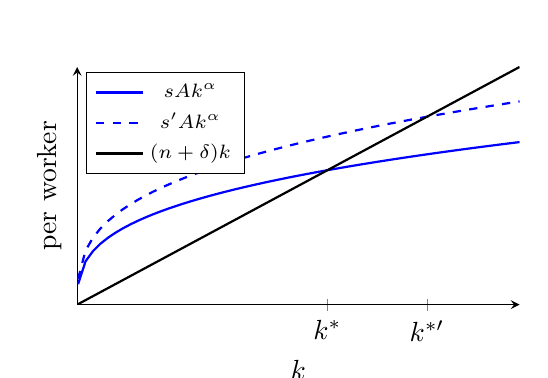
\begin{tikzpicture}
\begin{axis}[width=7.2cm,height=4.6cm,axis lines=left,xmin=0,xmax=5,ymin=0,ymax=0.5,xlabel={$k$},ylabel={per worker},
 xtick={2.828,3.953},xticklabels={$k^*$,$k^{*\prime}$},ytick=\empty,legend style={font=\scriptsize,at={(0.02,0.98)},anchor=north west},samples=60,domain=0.01:5]
\addplot[thick,blue]{0.20*x^(1/3)}; \addlegendentry{$sAk^{\alpha}$}
\addplot[thick,blue,dashed]{0.25*x^(1/3)}; \addlegendentry{$s'Ak^{\alpha}$}
\addplot[thick,black]{0.10*x}; \addlegendentry{$(n+\delta)k$}
\end{axis}
\end{tikzpicture}
\end{center}
\refbib{Kurlat (2020), \S4.2 (p.~57), Fig.~4.2.2.}
\rubrica{
\item $y^*$ and elasticity 0.5; first-period growth 0.5; consumption, long run and diagram 0.5. Saying long-run growth of $y$ rises: max.\ 0.5 pt.
Diagram without labelled curves or without the upward shift: $-0.25$ pt.
}
\end{sol}

\textbf{c)} (1.5 points) Two states share the calibration of (a): S\~ao Paulo sits at $k^*$ and Piau\'i starts at $k^*/8$. Find each state's growth
of $k$ and $y$ in the first period. Then let Piau\'i save only $s=0.10$: find its own steady state and its first-period growth, and say what
happens to $y_{PI}/y_{SP}$. Which kind of convergence does each case illustrate?
\resolespaco
\begin{sol}
\begin{notacao}
\item Symbols as in (a). $k_{PI}$, $y_{PI}$ and $k_{SP}$, $y_{SP}$: capital and output per worker in Piau\'i and S\~ao Paulo.
\item $s_{PI}=0.10$: Piau\'i's lower saving rate in the second case. $k^*_{PI}$, $y^*_{PI}$: its own steady state.
\end{notacao}
\passo{same parameters}{Piau\'i starts at $k_{PI}=2.8284/8=0.3536$. The term of \eqref{b2q5:ratio} that moves is}
\begin{align*}
k_{PI}^{\alpha-1}&=\Big(\frac{k^*}{8}\Big)^{-2/3}\\
&=(k^*)^{-2/3}\,8^{2/3}\\
&=0.5\times4=2 .
\end{align*}
Substitute into \eqref{b2q5:ratio} with $s=0.20$:
\begin{align*}
\frac{k_1}{k_0}&=\frac{(1-0.08)+0.20\times(1)\times(2)}{1+0.02}\\
&=\frac{0.92+0.20\times2}{1.02}\\
&=\frac{1.32}{1.02}=1.2941 .
\end{align*}
$k$ grows $29.4\%$; by \eqref{b2q5:y}, $y$ grows $1.2941^{1/3}-1=8.97\%$. S\~ao Paulo sits at $k^*$, where \eqref{b2q5:be} makes
\eqref{b2q5:ratio} equal to 1: it grows $0\%$. By \eqref{b2q5:y}, $y_{PI}=0.3536^{1/3}=2^{-1/2}=0.7071$ against $1.4142$: the poorer state
grows faster and the gap closes. Absolute convergence holds because both states share one steady state.
\passo{lower saving}{Piau\'i's own steady state: $s_{PI}/(n+\delta)=0.10/0.10=1$, so \eqref{b2q5:kss} and \eqref{b2q5:yss} give
$k^*_{PI}=y^*_{PI}=1$. At $k=0.3536$, \eqref{b2q5:ratio} with $s_{PI}$ gives}
\begin{align*}
\frac{k_1}{k_0}&=\frac{(1-0.08)+0.10\times(1)\times(2)}{1+0.02}\\
&=\frac{0.92+0.10\times2}{1.02}\\
&=\frac{1.12}{1.02}=1.0980 ,
\end{align*}
so $k$ grows $9.80\%$ and $y$ grows $1.0980^{1/3}-1=3.17\%$. It still grows, but toward its own lower level:
\[
\frac{y_{PI}}{y_{SP}}\ \text{rises from}\ \frac{0.7071}{1.4142}=0.5\ \text{to}\ \frac{1}{1.4142}=0.7071
\]
and stays there. Conditional convergence: growth depends on the distance from one's own steady state.
\intuicao{Diminishing returns make capital most productive where it is scarce; whether the poor catch up fully depends on
whether they share the rich economy's $s$, $n$, $\delta$ and $A$.}
\refbib{Kurlat (2020), \S3.3 (pp.~47--51) and Exercise~3.3 (p.~52); Exercise~5.2 (p.~94) on the speed of convergence.}
\rubrica{
\item Same-parameter growth rates 0.5; own steady state and growth 0.5; ratio and the absolute/conditional label 0.5.
Absolute convergence claimed for the low-saving case: max.\ 0.5 pt.
}
\end{sol}

% -----------------------------------------------------------------------------
\questao{(1 point) Multiple choice. Brazil's demographic transition lowers population growth $n$ from 2\% to 1\% a year for good. In
the Solow model without technological progress, starting and ending in steady state:}
\begin{alternativas}
\item $k^*$ and $y^*$ rise; long-run growth of $y$ stays at zero, while total GDP growth falls from 2\% to 1\% a year.
\item $k^*$ and $y^*$ rise; long-run growth of $y$ rises by one point, while total GDP growth stays at 2\% a year.
\item $k^*$ and $y^*$ fall; long-run growth of $y$ stays at zero, while total GDP growth stays at 2\% a year.
\item $k^*$ and $y^*$ rise; long-run growth of $y$ stays at zero, while total GDP growth stays at 2\% a year.
\item $k^*$ rises and $y^*$ stays put; long-run growth of $y$ stays at zero, while total GDP growth falls from 2\% to 1\% a year.
\end{alternativas}
\gabarito{A}
\begin{sol}
\begin{notacao}
\item Symbols as in Question~5; $g_Y$, $g_y$: growth rates of total GDP $Y$ and of GDP per worker $y=Y/L$.
\end{notacao}
\passo{levels}{By \eqref{b2q5:kss} and \eqref{b2q5:yss}, $k^*$ and $y^*$ both rise when $n$ falls: less investment goes to equipping new workers.}
\passo{growth}{Since $Y=yL$,}
\begin{equation}
1+g_Y=(1+g_y)(1+n). \label{b2q6:gY}
\end{equation}
In steady state $y$ is constant, $g_y=0$; substituting into \eqref{b2q6:gY}:
\begin{align*}
1+g_Y&=(1+0)(1+n)\\
g_Y&=n:
\end{align*}
total GDP growth falls from 2\% to 1\%. B confuses level with growth and
per capita with total (two mistakes); C gets the sign wrong and keeps total growth at 2\% (two); D keeps total growth at 2\%; E forgets that
$y^*=A(k^*)^{\alpha}$ moves with $k^*$.
\refbib{Kurlat (2020), \S4.2 (p.~57) and \S4.4 (p.~63).}
\end{sol}

% =============================================================================
% Block 3 --- Aula 3: Solow evidence (golden rule, technological progress, growth and TFP accounting).
% Weighted toward Prova 01 error cluster 2 (golden-rule algebra: carry the exponent, cross-check, knife edge).
\needspace{14\baselineskip}% keep the block heading, Q7's source line and its statement together
\bloco{3}{Solow continued: golden rule, TFP and growth accounting}{Aula 3 \,\textbullet\, Kurlat \S4.3--4.5, ch.~5 \,\textbullet\, 10 points}

\questao{(4 points) \textit{Source: Kurlat, P. (2020), \emph{A Course in Modern Macroeconomics}, Exercise 5.4 ``Measurement of the
Capital Stock'', pp.~94--95 --- statement reproduced verbatim, all items (a)--(d).}}

\noindent The capital stock is not easy to measure. A common way to try to do this is to:
\begin{itemize}[leftmargin=2.2em,topsep=2pt,itemsep=1pt]
\item guess a value for $K_0$ at some date in the past (maybe when statistics were first collected),
\item measure investment every year thereafter (which is also not that easy), and
\item use the equation
\[
K_{t+1}=(1-\delta)\,K_t+I_t \tag{5.5.1}
\]
to compute the capital stock for every year thereafter.
\end{itemize}
Consider an economy that is in a steady state without technological progress (and has been there for an infinitely long time).
Every year the level of investment is:
\[
I_t=0.2
\]
and the depreciation rate is:
\[
\delta=0.1
\]
\begin{enumerate}[label=(\alph*),leftmargin=2.2em,topsep=2pt,itemsep=1pt]
\item What is the capital stock?
\item The statistical office only started measuring investment in year 0. By then the economy was already in steady state. They
guessed (incorrectly) that the capital stock in year 0 was $K_0=1$. Use equation (5.5.1) to compute how the estimate of the capital
stock changed over time after year 0 and plot your answer. (You don't need to provide a closed form solution, a nice graph made
with a spreadsheet is enough). Compute the ratio:
\[
\frac{K_{ESTIMATE}}{K_{TRUE}}
\]
for the years 5, 10, and 50. (Again, you can just take the numbers from a spreadsheet).
\item Suppose now that the statistics office started collecting statistics a long time ago (an infinite time ago) so we don't have the
problem of making the wrong initial guess. However, instead of using the correct value of $\delta$, the statistical office incorrectly
believes that $\delta=0.05$. What is their estimate of the capital stock? Why does it differ from the truth?
\item The production function in this economy is
\[
Y=AK^{\alpha}L^{1-\alpha} \tag{5.5.2}
\]
and there are accurate data on GDP and on total hours of labor supply. Using the inaccurate estimate of $K$ from part (c), plus
accurate data on total labor and GDP, an economist is trying to measure the economy's productivity, i.e.\ to solve for $A$ in
equation (5.5.2). Find an expression for
\[
\frac{A_{ESTIMATE}}{A_{TRUE}}
\]
as a function of
\[
\frac{K_{ESTIMATE}}{K_{TRUE}}
\]
Given the numbers from part (c) and using $\alpha=0.35$, how far would the economist's estimate be from the truth?
\end{enumerate}
\noindent\textit{Changed by this list (not in the book):} for (b), give the closed form of the estimate, not only a spreadsheet.
\resolespaco
\begin{sol}
\begin{notacao}
\item $K_t$: capital stock; $I=0.2$: investment, constant every year; $\delta=0.1$: true depreciation rate.
\item $K^{TRUE}$: the true (steady-state) stock. $K^{EST}_t$: the statistician's estimate in year $t$, started from the guess $K^{EST}_0=1$.
\item $e_t\equiv K^{EST}_t-K^{TRUE}$: the estimation error. $\hat\delta=0.05$: the wrong depreciation rate of (c).
\item $A$: TFP, measured as a residual; $Y$, $L$: output and labour; $\alpha=0.35$: capital share.
\end{notacao}
\passo{(a) true stock}{Kurlat's perpetual-inventory equation (5.5.1), with constant investment:}
\begin{equation}
K_{t+1}=(1-\delta)K_t+I. \label{b3q7:pim}
\end{equation}
In a steady state $K_{t+1}=K_t=K$, so \eqref{b3q7:pim} gives
\begin{align*}
K&=(1-\delta)K+I\\
\delta K&=I\\
K^{TRUE}&=I/\delta=0.2/0.1=2 .
\end{align*}
\passo{(b) wrong initial guess}{The estimate and the truth both obey \eqref{b3q7:pim}. Subtracting one from the other, $I$ cancels:}
\begin{equation}
e_{t+1}=(1-\delta)\,e_t,\qquad e_0=1-2=-1. \label{b3q7:err}
\end{equation}
Iterating \eqref{b3q7:err} $t$ times:
\begin{align*}
e_t&=(1-\delta)^t e_0\\
&=(1-0.1)^t\,(-1)=-0.9^t,\\
K^{EST}_t&=K^{TRUE}+e_t\\
&=(2)+(-0.9^t)=2-0.9^t,\\
\frac{K^{EST}_t}{K^{TRUE}}&=\frac{(2-0.9^t)}{(2)}\\
&=1-\tfrac12\,0.9^t .
\end{align*}
Evaluating at the three dates:
\begin{center}\small
\begin{tabular}{@{}lccc@{}}
\toprule
Year $t$ & $0.9^t$ & $K^{EST}_t$ & $K^{EST}_t/K^{TRUE}$\\
\midrule
5 & 0.5905 & 1.4095 & 0.7048\\
10 & 0.3487 & 1.6513 & 0.8257\\
50 & 0.0052 & 1.9948 & 0.9974\\
\bottomrule
\end{tabular}
\end{center}
The guess is forgotten geometrically at rate $1-\delta$.
\passo{(c) wrong depreciation}{With $\hat\delta=0.05$ the perpetual inventory adds up every past vintage of investment, each
kept at the survival rate $1-\hat\delta$:}
\begin{align*}
K^{EST}&=\textstyle\sum_{j\ge0}(1-\hat\delta)^jI\\
&=I/\hat\delta=0.2/0.05=4,
\end{align*}
twice the truth: every vintage of investment is kept on the books twice as long as it really survives.
\passo{(d) TFP}{TFP is the residual of the production function:}
\begin{equation}
A=\frac{Y}{K^{\alpha}L^{1-\alpha}}. \label{b3q7:A}
\end{equation}
Dividing \eqref{b3q7:A} at $K^{EST}$ by \eqref{b3q7:A} at $K^{TRUE}$, with the same $Y$ and $L$:
\begin{align*}
\frac{A^{EST}}{A^{TRUE}}&=\frac{Y/\big[(K^{EST})^{\alpha}L^{1-\alpha}\big]}{Y/\big[(K^{TRUE})^{\alpha}L^{1-\alpha}\big]}\\
&=\Big(\frac{K^{EST}}{K^{TRUE}}\Big)^{-\alpha}\\
&=\Big(\frac{4}{2}\Big)^{-0.35}=2^{-0.35}=0.7846 :
\end{align*}
measured TFP is about $21.5\%$ too low.
\intuicao{TFP is a residual, so every error in measuring inputs lands in it with the opposite sign, damped by the input's share.}
\refbib{Kurlat (2020), \S5.4 (p.~86) and \S5.5 (p.~89). Consistent with the project's worked solution
(Problem 5.4, folder \texttt{Resolucao}); the book prints no answer.}
\rubrica{
\item (a) 0.5; (b) 1.5 (closed form 1, three ratios 0.5); (c) 1; (d) 1. Ratio in (d) written as $2^{\alpha}$ (sign of the bias reversed): max.\ 0.5 pt in (d).
}
\end{sol}

% -----------------------------------------------------------------------------
\questao{(5 points) Discursive. \emph{Golden rule $\times$ interest rates $\times$ dynamic efficiency.} Solow model in continuous time with
labour-augmenting technology: $Y=K^{\alpha}(AL)^{1-\alpha}$, $\dot A/A=g$, $\dot L/L=n$, depreciation $\delta$, saving rate $s$. Variables per
efficiency unit: $\tilde k=K/(AL)$, $\tilde y=\tilde k^{\alpha}$, $\tilde c=(1-s)\tilde y$, and $\dot{\tilde k}=s\tilde k^{\alpha}-(n+g+\delta)\tilde k$.
Competitive factor markets give $r=\alpha\tilde k^{\alpha-1}-\delta$. Illustrative calibration for Brazil: $\alpha=1/3$, $n=0.01$,
$g=0.02$, $\delta=0.05$, $s=0.18$.}

\textbf{a)} (2 points) Find steady-state $\tilde c^*(s)$ in closed form and the saving rate $s_{GR}$ that maximises it, with the second-order
condition. Cross-check with the capital-stock version of the problem, and use a knife-edge value of $\alpha$ to test your exponent.
\resolespaco
\begin{sol}
\begin{notacao}
\item $K$, $L$: capital and labour; $A$: labour-augmenting technology. $g\ge0$: growth of $A$; $n\ge0$: growth of $L$.
\item $\delta\in(0,1)$: depreciation. $s\in(0,1)$: saving rate. $\alpha\in(0,1)$: capital share.
\item $\tilde k\equiv K/(AL)$, $\tilde y$, $\tilde c$: capital, output and consumption per efficiency unit; a star marks the steady state.
\item $r$: real interest rate. $s_{GR}$: golden-rule saving rate. $\tilde k_{GR}$: golden-rule capital per efficiency unit.
\end{notacao}
\passo{the statement's equations}{Numbered here for reference:}
\begin{align}
\dot{\tilde k}&=s\tilde k^{\alpha}-(n+g+\delta)\tilde k, \label{b3q8:kdot}\\
\tilde y&=\tilde k^{\alpha},\qquad \tilde c=(1-s)\,\tilde y, \label{b3q8:yc}\\
r&=\alpha\tilde k^{\alpha-1}-\delta. \label{b3q8:r}
\end{align}
\passo{steady state}{Set $\dot{\tilde k}=0$ in \eqref{b3q8:kdot}:}
\begin{align}
s\tilde k^{\alpha}&=(n+g+\delta)\tilde k \label{b3q8:be}\\
\tilde k^{1-\alpha}&=\frac{s}{n+g+\delta}. \nonumber
\end{align}
Raise both sides to the power $1/(1-\alpha)$:
\begin{equation}
\tilde k^*=\Big(\frac{s}{n+g+\delta}\Big)^{\frac1{1-\alpha}}. \label{b3q8:kss}
\end{equation}
Substitute \eqref{b3q8:kss} into \eqref{b3q8:yc}:
\begin{align}
\tilde c^*(s)&=(1-s)(\tilde k^*)^{\alpha}\nonumber\\
&=(1-s)\Big(\Big(\frac{s}{n+g+\delta}\Big)^{\frac1{1-\alpha}}\Big)^{\alpha}\nonumber\\
&=(1-s)\Big(\frac{s}{n+g+\delta}\Big)^{\frac{\alpha}{1-\alpha}}. \label{b3q8:css}
\end{align}
The exponent is $\alpha/(1-\alpha)$, not $1/(1-\alpha)$: $\tilde k^*$ enters raised to $\alpha$.
\passo{first-order condition}{Take the log of \eqref{b3q8:css}:}
\begin{equation}
\ln\tilde c^*=\ln(1-s)+\frac{\alpha}{1-\alpha}\ln s-\frac{\alpha}{1-\alpha}\ln(n+g+\delta). \label{b3q8:ln}
\end{equation}
Differentiate \eqref{b3q8:ln} with respect to $s$ and set it to zero:
\begin{equation}
-\frac1{1-s}+\frac{\alpha}{(1-\alpha)s}=0. \label{b3q8:foc}
\end{equation}
Multiply \eqref{b3q8:foc} by $(1-\alpha)s(1-s)>0$:
\begin{align*}
\alpha(1-s)&=(1-\alpha)s\\
\alpha-\alpha s&=s-\alpha s\\
\alpha&=s .
\end{align*}
Hence
\begin{equation}
\boxed{s_{GR}=\alpha}. \label{b3q8:sgr}
\end{equation}
\passo{second-order condition}{Differentiate the left side of \eqref{b3q8:foc} once more:}
\[
\frac{d^2\ln\tilde c^*}{ds^2}=-\frac1{(1-s)^2}-\frac{\alpha}{(1-\alpha)s^2}<0 .
\]
At $s=\alpha$:
\begin{align*}
\frac{d^2\ln\tilde c^*}{ds^2}\Big|_{s=\alpha}&=-\frac1{(1-(\alpha))^2}-\frac{\alpha}{(1-\alpha)(\alpha)^2}\\
&=-\frac1{(1-\alpha)^2}-\frac{1}{(1-\alpha)\alpha}\\
&=-\frac{\alpha+(1-\alpha)}{\alpha(1-\alpha)^2}\\
&=-\frac1{\alpha(1-\alpha)^2}.
\end{align*}
A maximum.
\passo{cross-check}{Choose $\tilde k$ directly. By \eqref{b3q8:yc} and then \eqref{b3q8:be}, steady-state consumption is}
\begin{align}
\tilde c^*&=\tilde k^{\alpha}-s\tilde k^{\alpha}\nonumber\\
&=\tilde k^{\alpha}-(n+g+\delta)\tilde k. \label{b3q8:ck}
\end{align}
Maximising \eqref{b3q8:ck} over $\tilde k$:
\begin{equation}
\alpha\tilde k^{\alpha-1}=n+g+\delta, \label{b3q8:mpk}
\end{equation}
that is, MPK $=n+g+\delta$. Solve \eqref{b3q8:be} for $s$ and substitute \eqref{b3q8:mpk}:
\begin{align*}
s&=\frac{(n+g+\delta)\,\tilde k}{\tilde k^{\alpha}}\\
&=\frac{(\alpha\tilde k^{\alpha-1})\,\tilde k}{\tilde k^{\alpha}}\\
&=\alpha\tilde k^{\alpha-1}\,\tilde k^{1-\alpha}\\
&=\alpha .
\end{align*}
Same answer as \eqref{b3q8:sgr}.
\passo{knife edge}{As $\alpha\to0$ capital is useless, so $s_{GR}\to0$, as \eqref{b3q8:sgr} says. Dropping the $\alpha$ in the exponent
of \eqref{b3q8:css}, $\max(1-s)s^{1/(1-\alpha)}$ gives $s=1/(2-\alpha)\to1/2$: absurd, so the exponent is wrong.}
\refbib{Kurlat (2020), \S4.3 (p.~61) and \S4.5 (p.~69); Prova~01, Q2(b) (\texttt{Prova/}\allowbreak\texttt{prova-01-error-analysis.md}).}
\rubrica{
\item $\tilde c^*(s)$ with exponent $\alpha/(1-\alpha)$ 0.5; FOC and $s_{GR}$ 0.5; SOC 0.25; cross-check 0.5; knife edge 0.25.
Exponent $1/(1-\alpha)$ carried into the FOC: max.\ 0.75 pt. $s_{GR}$ confused with the $s$ that maximises $\tilde k^*$: max.\ 0.5 pt.
}
\end{sol}

\textbf{b)} (1.5 points) Compute $\tilde k^*$, $\tilde c^*$ and $r$ at $s=0.18$ and at $s_{GR}$. Show that $r-(n+g)$ has the sign of $\alpha-s$, and say
whether Brazil should raise its saving rate.
\resolespaco
\begin{sol}
\begin{notacao}
\item Symbols as in (a); calibration $\alpha=1/3$, $n=0.01$, $g=0.02$, $\delta=0.05$.
\end{notacao}
\passo{numbers}{Here $n+g+\delta=0.08$, $\frac{\alpha}{1-\alpha}=\frac12$ and $\frac1{1-\alpha}=\frac32$. Using \eqref{b3q8:kss} and \eqref{b3q8:css}
at $s=0.18$, where $s/0.08=2.25$:}
\begin{align*}
\tilde k^*&=\Big(\frac{0.18}{0.01+0.02+0.05}\Big)^{3/2}\\
&=2.25^{3/2}=3.375,\\
\tilde c^*&=(1-0.18)\Big(\frac{0.18}{0.01+0.02+0.05}\Big)^{1/2}\\
&=0.82\times2.25^{1/2}=0.82\times1.5=1.23 .
\end{align*}
At $s=1/3$, where $s/0.08=4.1667$:
\begin{align*}
\tilde k^*&=\Big(\frac{1/3}{0.08}\Big)^{3/2}\\
&=4.1667^{3/2}=8.5052,\\
\tilde c^*&=\Big(1-\frac13\Big)\Big(\frac{1/3}{0.08}\Big)^{1/2}\\
&=\tfrac23\times4.1667^{1/2}=\tfrac23\times2.0412=1.3608 .
\end{align*}
The ratio is $1.3608/1.23=1.106$: $10.6\%$ more consumption per efficiency unit.
\passo{interest rate}{Divide \eqref{b3q8:be} by $s\tilde k$:}
\begin{equation}
\tilde k^{\alpha-1}=\frac{n+g+\delta}{s}. \label{b3q8:kam1}
\end{equation}
Substitute \eqref{b3q8:kam1} into \eqref{b3q8:r}:
\begin{align}
r&=\alpha\Big(\frac{n+g+\delta}{s}\Big)-\delta\nonumber\\
&=\frac{\alpha(n+g+\delta)}{s}-\delta. \label{b3q8:rs}
\end{align}
Subtract $n+g$ from both sides of \eqref{b3q8:rs}:
\begin{align*}
r-(n+g)&=\frac{\alpha(n+g+\delta)}{s}-(n+g+\delta)\\
&=(n+g+\delta)\Big(\frac{\alpha}{s}-1\Big),
\end{align*}
positive iff $s<\alpha$. Using \eqref{b3q8:rs} at each saving rate:
\begin{align*}
s=0.18:\quad r&=\tfrac13\times\tfrac{0.08}{0.18}-0.05=0.1481-0.05=0.0981>0.03,\\
s=1/3:\quad r&=\tfrac13\times\tfrac{0.08}{(1/3)}-0.05\\
&=0.08-0.05=0.03=n+g .
\end{align*}
The golden rule is $r=n+g$.
\passo{policy}{Brazil is below the golden rule and dynamically efficient. Raising $s$ to $1/3$ raises long-run consumption, but
consumption falls on impact and for a while along the transition: generations are traded off, and Solow, with no preferences,
cannot say whether the sacrifice is worth it. That is the job of the microfounded models of Aulas 4--6.}
\refbib{Kurlat (2020), \S4.3 (p.~61) and \S4.4 (p.~63); Exercise~5.8 (p.~97).}
\rubrica{
\item Numbers 0.5; $r-(n+g)$ sign 0.5; policy reading 0.5. Concluding that being below the golden rule is inefficient: max.\ 0.25 pt for the reading.
}
\end{sol}

\textbf{c)} (1.5 points) Another economy has the same parameters but $s=0.45$. Show that cutting $s$ to $\alpha$ raises consumption per
efficiency unit on impact and at every later date, and name the inefficiency.
\resolespaco
\begin{sol}
\begin{notacao}
\item Symbols as in (a). $\tilde k_0$: capital per efficiency unit when $s$ is cut; $\tilde c_t$, $\tilde k_t$: values along the transition.
\item $f(\tilde k)\equiv\tilde k^{\alpha}-(n+g+\delta)\tilde k$: steady-state consumption as a function of $\tilde k$, the right side of \eqref{b3q8:ck}.
\end{notacao}
\passo{diagnosis}{At $s=0.45$, $s/0.08=5.625$. Using \eqref{b3q8:kss}, \eqref{b3q8:css} and \eqref{b3q8:rs}:}
\begin{align*}
\tilde k^*&=\Big(\frac{0.45}{0.08}\Big)^{3/2}\\
&=5.625^{3/2}=13.3409,\\
\tilde c^*&=(1-0.45)\Big(\frac{0.45}{0.08}\Big)^{1/2}\\
&=0.55\times5.625^{1/2}=0.55\times2.3717=1.3044<1.3608,\\
r&=\tfrac13\times\tfrac{0.08}{0.45}-0.05=0.0093<n+g=0.03 .
\end{align*}
\passo{impact}{$\tilde k$ is predetermined, so by \eqref{b3q8:yc} $\tilde y=2.3717$ on impact and $\tilde c$ jumps:}
\[
\tilde c:\ 0.55\times2.3717=1.3044\ \longrightarrow\ \tfrac23\times2.3717=1.5811 .
\]
\passo{transition}{Using \eqref{b3q8:yc} and then \eqref{b3q8:kdot} for $s\tilde k^{\alpha}$, consumption along the path is}
\begin{align}
\tilde c_t&=\tilde k_t^{\alpha}-s\tilde k_t^{\alpha}\nonumber\\
&=\tilde k_t^{\alpha}-\big(\dot{\tilde k}_t+(n+g+\delta)\tilde k_t\big)\nonumber\\
&=\tilde k_t^{\alpha}-(n+g+\delta)\tilde k_t-\dot{\tilde k}_t\nonumber\\
&=f(\tilde k_t)-\dot{\tilde k}_t. \label{b3q8:cpath}
\end{align}
With $s=\alpha$, $\tilde k$ falls monotonically from $13.3409$ to $\tilde k_{GR}=8.5052$, so $\dot{\tilde k}_t<0$. On
$(\tilde k_{GR},13.3409]$, $f$ is decreasing: $f'(\tilde k)=\alpha\tilde k^{\alpha-1}-(n+g+\delta)$ is negative above $\tilde k_{GR}$ by
\eqref{b3q8:mpk}. So $\tilde k_t<\tilde k_0$ gives $f(\tilde k_t)>f(\tilde k_0)$, and \eqref{b3q8:cpath} gives
\[
\tilde c_t>f(\tilde k_t)>f(\tilde k_0)=1.3044\quad\text{at every }t,
\]
ending at $1.3608$.
\passo{name}{Every date gains and none loses: a Pareto improvement. The economy over-accumulates capital, $r<n+g$:
\textbf{dynamic inefficiency}.}
\refbib{Kurlat (2020), \S4.3 (p.~61); Romer (2012), \S1.4 and \S2.11 (pp.~88--91).}
\rubrica{
\item Diagnosis 0.25; impact 0.5; transition argument 0.5; name 0.25. Asserting the path without the monotonicity argument: max.\ 0.25 pt for it.
}
\end{sol}

% -----------------------------------------------------------------------------
\questao{(1 point) Multiple choice. Illustrative Brazilian data, 2000--2014 averages: GDP grows $3.2\%$, the capital stock $4.4\%$ and hours
$1.8\%$ a year; the capital share is $0.4$. The Solow residual, and the share of the growth of output \emph{per hour} it accounts for, are:}
\begin{alternativas}
\item $0.36$ p.p.\ a year, accounting for about 11\% of the growth of output per hour.
\item $-0.16$ p.p.\ a year, accounting for about $-5\%$ of the growth of output per hour.
\item $1.44$ p.p.\ a year, accounting for about 45\% of the growth of output per hour.
\item $0.36$ p.p.\ a year, accounting for about 26\% of the growth of output per hour.
\item $0.56$ p.p.\ a year, accounting for about 40\% of the growth of output per hour.
\end{alternativas}
\gabarito{D}
\begin{sol}
\begin{notacao}
\item $g_Y$, $g_K$, $g_L$, $g_A$: growth of output, capital, hours and TFP (p.p.\ a year); $g_y$: growth of output per hour; $\alpha=0.4$: capital share.
\end{notacao}
\passo{residual}{Kurlat's growth-accounting equation (5.4.2):}
\begin{equation}
g_A=g_Y-\alpha g_K-(1-\alpha)g_L. \label{b3q9:ga}
\end{equation}
Substituting the data into \eqref{b3q9:ga}:
\begin{align*}
g_A&=3.2-0.4\times4.4-0.6\times1.8\\
&=3.2-1.76-1.08=0.36 .
\end{align*}
\passo{per hour}{Output per hour grows at $g_y=g_Y-g_L=3.2-1.8=1.4$. Subtracting $g_L$ from both sides of \eqref{b3q9:ga} and rearranging:}
\begin{align*}
g_y&=g_A+\alpha(g_K-g_L)\\
&=(0.36)+0.4\times(4.4-1.8)\\
&=0.36+0.4\times2.6=0.36+1.04=1.4 .
\end{align*}
The residual's share is $0.36/1.4=25.7\%$.
\passo{distractors}{A divides by output growth ($0.36/3.2$); B swaps the shares ($3.2-2.64-0.72$) and divides by $3.2$ (two mistakes);
C drops labour ($3.2-1.76$) and divides by $3.2$ (two); E swaps the shares and drops labour ($3.2-2.64$), divided by $1.4$ (two).}
\refbib{Kurlat (2020), \S5.4, eq.~(5.4.2) (p.~86).}
\end{sol}

% =============================================================================
% Block 4 --- Aula 4: consumption and saving (two-period problem, Euler, Ricardian equivalence, credit constraints).
% Weighted toward Prova 01 error cluster 3 (list every choice variable and every income source).
\bloco{4}{Consumption and saving}{Aula 4 \,\textbullet\, Kurlat ch.~6 \,\textbullet\, 10 points}

\questao{(4 points) \textit{Source: Kurlat, P. (2020), \emph{A Course in Modern Macroeconomics}, Exercise 6.4 ``Consumption and
Income'', pp.~122--123 --- statement reproduced verbatim, all items (a)--(d).}}

\noindent Suppose there are two households in the economy. Each of them solves a special case of Exercise 6.1, where
$\tau_1=\tau_2=a_0=0$, $\beta=1$ and $r=0$.
\begin{enumerate}[label=(\alph*),leftmargin=2.2em,topsep=2pt,itemsep=1pt]
\item Solve for $c_1$ as a function of $y_1$ and $y_2$.
\item Suppose the incomes of each of the households are:
\begin{center}\small
\begin{tabular}{@{}lcc@{}}
\toprule
 & $y_1$ & $y_2$ \\
\midrule
Household A & 2 & 4 \\
Household B & 6 & 4 \\
\bottomrule
\end{tabular}
\end{center}
Compute $c_1$ and $c_2$ for each of the households.
\item Suppose an economist is trying to decide what is a reasonable model for consumption behavior and only has data for period 1. Is
the data supportive of the Keynesian view of the consumption function? Explain.
\item Suppose the same economist now looks at data for period 2 in addition to data for period 1. Is the data supportive of the
Keynesian view of the consumption function? Explain.
\end{enumerate}
\noindent\textit{Our note, not in the book:} Kurlat's Exercise 6.1 (p.~121) is $\max_{c_1,a,c_2}u(c_1)+\beta u(c_2)$ s.t.\
$a=a_0+y_1-\tau_1-c_1$ and $c_2=y_2-\tau_2+(1+r)a$, with $u(c)=\frac{c^{1-\sigma}}{1-\sigma}$.\par
\noindent\textit{Added to the book's items (not in the book):} in (c) and (d), fit the line $c=a+by$ that a Keynesian economist would
estimate and say what it does and does not show.
\resolespaco
\begin{sol}
\begin{notacao}
\item $c_t$, $y_t$: consumption and income in period $t\in\{1,2\}$. $\beta=1$: discount factor. $r=0$: interest rate.
\item $u$: strictly increasing and strictly concave period utility (CRRA with curvature $\sigma>0$ in Exercise~6.1).
\item $a$, $b$: intercept and slope of the Keynesian line $c=a+by$; $\bar y$, $\bar c$: sample means.
\end{notacao}
\passo{(a)}{Exercise~6.1 with $\tau_1=\tau_2=a_0=0$ gives the Euler equation and the budget constraint:}
\begin{align}
u'(c_1)&=\beta(1+r)\,u'(c_2), \label{b4q10:euler}\\
c_1+\frac{c_2}{1+r}&=y_1+\frac{y_2}{1+r}. \label{b4q10:bc}
\end{align}
Substituting $\beta=1$ and $r=0$ into \eqref{b4q10:euler}:
\begin{align*}
u'(c_1)&=(1)(1+(0))\,u'(c_2)\\
u'(c_1)&=u'(c_2).
\end{align*}
$u$ is strictly concave, so $u'$ is strictly decreasing and
$c_1=c_2$ for any $\sigma$. Substituting $c_2=c_1$ into \eqref{b4q10:bc} with $r=0$:
\begin{align}
c_1+\frac{(c_1)}{1+(0)}&=y_1+\frac{y_2}{1+(0)}\nonumber\\
2c_1&=y_1+y_2\nonumber\\
c_1=c_2&=\frac{y_1+y_2}{2}. \label{b4q10:c}
\end{align}
\passo{(b)}{Using \eqref{b4q10:c} for each household:}
\begin{align*}
\text{A:}\quad c_1=c_2&=(2+4)/2=3,\qquad y_1-c_1=2-3=-1,\\
\text{B:}\quad c_1=c_2&=(6+4)/2=5,\qquad y_1-c_1=6-5=1 .
\end{align*}
A borrows $1$ in period 1; B saves $1$.
\passo{(c) period-1 data}{The line through $(y,c)=(2,3)$ and $(6,5)$:}
\begin{align*}
b&=\frac{5-3}{6-2}=0.5,\\
a&=3-0.5\times2=2 .
\end{align*}
So $c=2+0.5\,y$: a positive intercept, a marginal propensity of $0.5<1$, and an average propensity that falls with income
($3/2=1.5$ against $5/6=0.83$). On its face this is Keynes's consumption function. But the slope is not a behavioural response:
income differences in period 1 are partly temporary, and by \eqref{b4q10:c} each household consumes its \emph{average} income.
\passo{(d) both periods}{In period 2 both incomes are $4$ while consumption is $3$ and $5$: current income does not explain
consumption at all. Over time A's income doubles ($2\to4$) and B's falls ($6\to4$), and neither household changes $c$: the
time-series propensity to consume out of these anticipated income changes is zero. Pooling the four observations, the least-squares
line is}
\begin{equation}
b=\frac{\mathrm{cov}(y,c)}{\mathrm{var}(y)},\qquad a=\bar c-b\,\bar y. \label{b4q10:ols}
\end{equation}
With $y=(2,6,4,4)$ and $c=(3,5,3,5)$: $\bar y=4$, $\bar c=4$, $\mathrm{cov}(y,c)=1$, $\mathrm{var}(y)=2$. Using \eqref{b4q10:ols}:
\begin{align*}
b&=1/2=0.5,\\
a&=4-0.5\times4=2 .
\end{align*}
The pooled line is still $c=2+0.5\,y$, yet it fits no household's behaviour: the data reject the Keynesian function and support the
permanent-income view of \eqref{b4q10:c}, where $c$ depends on lifetime resources ($y_1+y_2=6$ for A and $10$ for B).
\intuicao{A cross-section confounds permanent and temporary income; consumption responds to the first, so a Keynesian slope fitted
on one year of data measures how much income variation is permanent, not how households react to income.}
\refbib{Kurlat (2020), \S6.1 (p.~103) and \S6.2 (p.~105), eqs.~(6.2.10)--(6.2.11). Consistent with the project's worked solution
(Problem 6.4, folder \texttt{Resolucao}); the book prints no answer.}
\rubrica{
\item (a) 1; (b) 1; (c) 1; (d) 1. Calling the period-1 slope the households' MPC without qualification: max.\ 0.5 pt in (c).
}
\end{sol}

% -----------------------------------------------------------------------------
\questao{(5 points) Discursive. \emph{Choice variables $\times$ Ricardian equivalence $\times$ credit constraints.} A Brazilian worker lives two
periods (working life and retirement, about 30 years each) with utility $\ln c_1+\beta\ln c_2$, $\beta=0.6$. In period 1 she holds initial
wealth $a_0=10$, earns labour income $w_1=40$ (hours are fixed), receives dividends $\Pi_1=10$ from the family firm she owns and pays a
lump-sum tax $\tau_1=10$. In period 2 she receives income $y_2=90$ and pays $\tau_2=10$. She borrows or lends $a$ at the gross rate
$1+r=2$ (about $2.3\%$ a year over 30 years).}

\textbf{a)} (2 points) List every choice variable and every source of income. Write the two period budget constraints and the
intertemporal one, set up the Lagrangian, derive the first-order conditions and the Euler equation, and find $c_1$, $c_2$ and $a$.
\resolespaco
\begin{sol}
\begin{notacao}
\item $c_1$, $c_2>0$: consumption in working life and in retirement. $a\in\mathbb R$: assets carried into period 2 ($a<0$ is borrowing).
\item $a_0=10$: initial wealth. $w_1=40$: labour income. $\Pi_1=10$: dividends. $y_2=90$: period-2 income. $\tau_1$, $\tau_2$: lump-sum taxes.
\item $\beta\in(0,1)$: discount factor, $0.6$. $r$: interest rate over the period, $1+r=2$.
\item $W$: lifetime resources in present value. $\lambda>0$: multiplier on the intertemporal budget.
\end{notacao}
\passo{choices and income}{Choice variables: $c_1$, $c_2$, $a$ (a negative $a$ is borrowing). Income: initial wealth $a_0$, labour income
$w_1$, profits $\Pi_1$ (she owns the firm), period-2 income $y_2$; taxes $\tau_1$, $\tau_2$ are paid out of them.}
\passo{constraints}{Resources equal uses in each period:}
\begin{align}
c_1+a&=a_0+w_1+\Pi_1-\tau_1, \label{b4q11:bc1}\\
c_2&=y_2-\tau_2+(1+r)\,a. \label{b4q11:bc2}
\end{align}
Solve \eqref{b4q11:bc2} for $a$:
\[
a=\frac{c_2-y_2+\tau_2}{1+r}.
\]
Substitute this into \eqref{b4q11:bc1}:
\[
c_1+\Big(\frac{c_2-y_2+\tau_2}{1+r}\Big)=a_0+w_1+\Pi_1-\tau_1 .
\]
Collect the terms in $c_2$ on the left:
\begin{equation}
c_1+\frac{c_2}{1+r}=a_0+w_1+\Pi_1-\tau_1+\frac{y_2-\tau_2}{1+r}\equiv W. \label{b4q11:ibc}
\end{equation}
With the data:
\[
W=10+40+10-10+\frac{90-10}{2}=50+40=90 .
\]
\passo{Lagrangian and FOCs}{Maximise utility subject to \eqref{b4q11:ibc}:}
\begin{equation}
\mathcal L=\ln c_1+\beta\ln c_2+\lambda\Big[W-c_1-\frac{c_2}{1+r}\Big]. \label{b4q11:L}
\end{equation}
Differentiate \eqref{b4q11:L} with respect to $c_1$ and $c_2$:
\begin{align}
\frac1{c_1}&=\lambda, \label{b4q11:foc1}\\
\frac{\beta}{c_2}&=\frac{\lambda}{1+r}. \label{b4q11:foc2}
\end{align}
Substitute $\lambda$ from \eqref{b4q11:foc1} into \eqref{b4q11:foc2} and rearrange:
\begin{align}
\frac{\beta}{c_2}&=\frac{(1/c_1)}{1+r}\nonumber\\
\frac{\beta}{c_2}&=\frac{1}{(1+r)\,c_1}\nonumber\\
c_2&=\beta(1+r)\,c_1. \label{b4q11:euler}
\end{align}
With the data, $c_2=0.6\times2\times c_1=1.2\,c_1$.
\passo{solution}{Substitute \eqref{b4q11:euler} into \eqref{b4q11:ibc}:}
\begin{align*}
c_1+\frac{\big(\beta(1+r)\,c_1\big)}{1+r}&=W\\
c_1+\beta c_1&=W\\
(1+\beta)\,c_1&=W,
\end{align*}
so
\begin{equation}
c_1=\frac{W}{1+\beta}=\frac{90}{1.6}=56.25. \label{b4q11:c1}
\end{equation}
Then \eqref{b4q11:euler} and \eqref{b4q11:bc1} give
\begin{align*}
c_2&=1.2\times(56.25)=67.5,\\
a&=10+40+10-10-(56.25)\\
&=50-56.25=-6.25 .
\end{align*}
Check with \eqref{b4q11:bc2}: $c_2=80+2\times(-6.25)=67.5$.
\intuicao{She consumes the fraction $1/(1+\beta)$ of lifetime wealth whatever its timing; her income is back-loaded ($y_2$ is large), so
smoothing makes her a borrower.}
\refbib{Kurlat (2020), \S6.2 (p.~105) and Exercise~6.1 (p.~121). The closed form of $c_1$ is the $\sigma=1$ case of the instructor's
solution to Lista~3, Q1(a) (\texttt{Listas/solu\c{c}\~oes do instrutor/PSET 3 (1).pdf}).}
\rubrica{
\item Choice variables and income sources 0.5; constraints and $W$ 0.5; FOCs and Euler 0.5; $c_1,c_2,a$ with check 0.5.
Profits $\Pi_1$ or $a_0$ omitted from the budget (the Prova~01 Q2(c) error): max.\ 1 pt. Discounting $c_2$ by $(1+r)$ in the wrong direction: max.\ 0.5 pt.
}
\end{sol}

\textbf{b)} (1.5 points) The government cuts $\tau_1$ to $0$, finances the gap by selling bonds and repays them with interest by raising $\tau_2$ to
$30$. Find the new $c_1$, $c_2$ and $a$, the change in private, public and national saving, and the assumptions the result needs.
\resolespaco
\begin{sol}
\begin{notacao}
\item Symbols as in (a); a prime marks values after the tax change ($\tau_1'=0$, $\tau_2'=30$).
\item $S^p$, $S^g$, $S$: private, public and national saving in period 1, with $S=S^p+S^g$.
\end{notacao}
\passo{wealth}{Using \eqref{b4q11:ibc} with the new taxes:}
\[
W'=10+40+10-0+\frac{90-30}{2}=60+30=90=W .
\]
The tax cut of $10$ is matched by a tax rise of $20=10\times(1+r)$, the same in present value.
\passo{choices}{$W$, $\beta$ and $r$ are unchanged, so \eqref{b4q11:c1} and \eqref{b4q11:euler} give $c_1=56.25$ and $c_2=67.5$. By \eqref{b4q11:bc1}:}
\begin{align*}
a'&=10+40+10-0-(56.25)\\
&=60-56.25=3.75 ,
\end{align*}
so $a$ rises by exactly $10$, the bonds she buys.
\passo{saving}{The changes in period 1:}
\begin{align*}
\Delta S^p&=\Delta a=3.75-(-6.25)=10,\\
\Delta S^g&=\Delta\tau_1=-10\ \text{(the deficit)},\\
\Delta S&=10-10=0 .
\end{align*}
National saving is unchanged: Ricardian equivalence.
\passo{assumptions}{Lump-sum taxes; the government and the household borrow at the same $r$; the taxpayer who gets the cut pays the
later tax (same horizon); she can borrow and lend freely at $r$.}
\refbib{Kurlat (2020), \S6.2, ``Taxes and Ricardian Equivalence''; Exercise~6.5 (p.~123).}
\rubrica{\item Wealth 0.5; choices 0.5; saving and assumptions 0.5. Claiming $c_1$ rises: max.\ 0.5 pt.}
\end{sol}

\textbf{c)} (1.5 points) Now she cannot borrow: $a\ge0$. Solve her problem before and after the tax change of (b). Does Ricardian equivalence hold?
What is her marginal propensity to consume out of the tax cut?
\resolespaco
\begin{sol}
\begin{notacao}
\item Symbols as in (a). $\mu\ge0$: multiplier on the borrowing constraint $a\ge0$.
\end{notacao}
\passo{the problem}{Substitute \eqref{b4q11:bc1} and \eqref{b4q11:bc2} for $c_1$ and $c_2$, so that $a$ is the only choice:}
\begin{equation}
\mathcal L=\ln\big(a_0+w_1+\Pi_1-\tau_1-a\big)+\beta\ln\big(y_2-\tau_2+(1+r)a\big)+\mu\,a. \label{b4q11:Lc}
\end{equation}
Differentiate \eqref{b4q11:Lc} with respect to $a$:
\begin{equation}
-\frac1{c_1}+\frac{\beta(1+r)}{c_2}+\mu=0,\qquad \mu\ge0,\qquad \mu\,a=0. \label{b4q11:foca}
\end{equation}
\passo{before}{The unconstrained choice $a=-6.25$ violates $a\ge0$, so the constraint binds: $a=0$, and \eqref{b4q11:bc1}--\eqref{b4q11:bc2} give}
\begin{align*}
c_1&=a_0+w_1+\Pi_1-\tau_1-(0)\\
&=10+40+10-10=50,\\
c_2&=y_2-\tau_2+(1+r)(0)\\
&=90-10=80 .
\end{align*}
Solve \eqref{b4q11:foca} for $\mu$:
\begin{align*}
\mu&=\frac1{c_1}-\frac{\beta(1+r)}{c_2}\\
&=\frac1{50}-\frac{1.2}{80}=0.02-0.015=0.005>0 .
\end{align*}
The Euler equation holds as an inequality, $u'(c_1)>\beta(1+r)u'(c_2)$.
\passo{after}{Period-1 resources are $60$ and the unconstrained choice of (b) gives $a=3.75\ge0$: the constraint no longer binds
($\mu=0$ in \eqref{b4q11:foca}, which is then the Euler equation \eqref{b4q11:euler}), so $c_1=56.25$, $c_2=67.5$.}
\passo{equivalence fails}{$c_1$ rises from $50$ to $56.25$ out of a tax cut that leaves $W$ unchanged:}
\[
\text{MPC}=\frac{56.25-50}{10}=0.625 .
\]
The cut works as a loan from the government that the market would not give her.
\intuicao{Credit-constrained households consume current income, so the timing of taxes matters for them and a debt-financed transfer
raises demand.}
\refbib{Kurlat (2020), Exercise~6.5 \emph{Credit Constraints and Ricardian Equivalence} (p.~123); \S6.2, ``Taxes and Ricardian Equivalence''.}
\rubrica{
\item Before 0.5 (with the inequality); after 0.5; MPC and conclusion 0.5. Imposing the Euler equality while the constraint binds: max.\ 0.5 pt.
}
\end{sol}

% -----------------------------------------------------------------------------
\questao{(1 point) Multiple choice. A household with $u(c)=c^{1-\sigma}/(1-\sigma)$, $\sigma>0$, has income only in period 1 ($y_1>0$, $y_2=0$, no
taxes, no initial wealth) and saves at rate $r$. When $r$ rises, $\partial c_1/\partial r$:}
\begin{alternativas}
\item is negative for every $\sigma>0$: a higher $r$ makes future consumption cheaper, so she saves more.
\item is positive iff $\sigma>1$: for a saver, the income effect of $r$ then outweighs the substitution effect.
\item is positive iff $\sigma<1$: an elasticity of intertemporal substitution above one makes the income effect dominate.
\item is zero for every $\sigma>0$: with $y_2=0$ there is no future income for a change in $r$ to revalue.
\item is negative iff $\sigma>1$: $\sigma$ is the elasticity of intertemporal substitution, so a large $\sigma$ makes substitution dominate.
\end{alternativas}
\gabarito{B}
\begin{sol}
\begin{notacao}
\item $c_1$, $c_2$: consumption; $y_1>0$: period-1 income; $\beta\in(0,1)$: discount factor; $r>-1$: interest rate;
$\sigma>0$: curvature of $u$, so $1/\sigma$ is the EIS; $D$: defined in \eqref{b4q12:c1}.
\end{notacao}
\passo{closed form}{The CRRA Euler equation and the budget constraint with $y_2=0$:}
\begin{align}
c_2&=[\beta(1+r)]^{1/\sigma}c_1, \label{b4q12:euler}\\
c_1+\frac{c_2}{1+r}&=y_1. \label{b4q12:bc}
\end{align}
Substitute \eqref{b4q12:euler} into \eqref{b4q12:bc}:
\begin{align}
c_1+\frac{\big([\beta(1+r)]^{1/\sigma}c_1\big)}{1+r}&=y_1\nonumber\\
c_1\big[1+\beta^{1/\sigma}(1+r)^{\frac1\sigma-1}\big]&=y_1\nonumber\\
c_1=\frac{y_1}{D},\qquad D&\equiv1+\beta^{1/\sigma}(1+r)^{\frac1\sigma-1}. \label{b4q12:c1}
\end{align}
\passo{sign}{Differentiate \eqref{b4q12:c1} with respect to $r$:}
\begin{align*}
\frac{\partial c_1}{\partial r}&=-\frac{y_1}{D^2}\,\frac{\partial D}{\partial r}\\
&=-\frac{y_1}{D^2}\,\Big(\beta^{1/\sigma}\Big(\frac1\sigma-1\Big)(1+r)^{\frac1\sigma-2}\Big)\\
&=\frac{y_1\beta^{1/\sigma}(1+r)^{\frac1\sigma-2}}{D^2}\cdot\frac{\sigma-1}{\sigma}.
\end{align*}
The first factor is positive, so the derivative is
positive iff $\sigma>1$, zero at $\sigma=1$ (log), negative iff $\sigma<1$. The EIS is $1/\sigma$; with $\sigma>1$ it is below one and the income
effect wins. A is the substitution effect alone; C reverses the condition; D ignores that $r$ also raises her interest income; E reverses
the sign and calls $\sigma$ the EIS (two mistakes).
\refbib{Kurlat (2020), \S6.2 (p.~105) and Exercises~6.1(e), 6.3 (pp.~121--122). Confirmed by the instructor's solution to Lista~3,
Q1(c): $\partial c_1/\partial r$ has the sign of $(\sigma-1)/\sigma$ (\texttt{PSET 3 (1).pdf}).}
\end{sol}

% =============================================================================
% Block 5 --- Aula 5: labour and leisure (static supply, income vs substitution, taxes, Frisch, search).
% Weighted toward Prova 01 error cluster 3 (every choice variable has a first-order condition; corners count).
\bloco{5}{Labour and leisure}{Aula 5 \,\textbullet\, Kurlat ch.~7 \,\textbullet\, 10 points}

\questao{(4 points) \textit{Source: Kurlat, P. (2020), \emph{A Course in Modern Macroeconomics}, Exercise 7.3 ``Consumption Taxes and
Labor Supply'', pp.~147--148 --- statement reproduced verbatim, all items (a)--(e).}}

\noindent Suppose a household solves the following problem:
\begin{align*}
&\max_{c,l}\ u(c)+v(l)\\
s.t.\quad &(1+\tau_c)\,c\le w(1-\tau)(1-l)
\end{align*}
where $c$ is consumption, $l$ is leisure and $\tau$ is an income tax. $\tau_c$ is a consumption tax, so that if the household wishes to
consume $c$ it must pay $(1+\tau_c)\,c$.
\begin{enumerate}[label=(\alph*),leftmargin=2.2em,topsep=2pt,itemsep=1pt]
\item Draw the household's budget constraint. What is the slope?
\item Find the first-order conditions for the household's consumption-leisure decision. How do the effects of $\tau$ and $\tau_c$
relate to each other? Explain.
\item If the household chooses $c^*$ and $l^*$, how much tax revenue does the government collect?
\item Suppose the government had originally set $\tau_c=0$ and $\tau>0$ and now wants to enact a tax reform that uses consumption
taxes instead of income taxes. What would be the level of $\tau_c$ that leaves the decisions of the household unchanged?
\item How much revenue does the government collect under the new system? How does it compare to the old system? Explain.
\end{enumerate}
\noindent\textit{Added to the book's items (not in the book):} in (d), also give the consumption tax that replaces a 30\% income tax.
\resolespaco
\begin{sol}
\begin{notacao}
\item $c\ge0$: consumption. $l\in[0,1]$: leisure; $1-l$: hours worked. $w>0$: wage.
\item $\tau\in[0,1)$: labour-income tax. $\tau_c\ge0$: consumption tax. $u$, $v$: increasing, concave utilities of $c$ and $l$.
\item $\lambda>0$: multiplier on the budget. $c^*$, $l^*$: the optimal choices. $R$, $R'$: tax revenue under the income and the consumption tax.
\end{notacao}
\passo{(a) budget line}{Spending on consumption, taxes included, equals after-tax labour income:}
\begin{equation}
(1+\tau_c)\,c=w(1-\tau)(1-l). \label{b5q13:bc}
\end{equation}
Solving \eqref{b5q13:bc} for $c$:
\[
c=\frac{w(1-\tau)}{1+\tau_c}\,(1-l).
\]
With $l$ on the horizontal axis and $c$ on the vertical, this is a line from $(l,c)=(1,0)$ to $\big(0,\frac{w(1-\tau)}{1+\tau_c}\big)$, with slope
$\dfrac{dc}{dl}=-\dfrac{w(1-\tau)}{1+\tau_c}$: the real after-tax wage in units of consumption.
\passo{(b) first-order conditions}{Maximise $u(c)+v(l)$ subject to \eqref{b5q13:bc}:}
\begin{equation}
\mathcal L=u(c)+v(l)-\lambda\big[(1+\tau_c)c-w(1-\tau)(1-l)\big]. \label{b5q13:L}
\end{equation}
Differentiate \eqref{b5q13:L} with respect to $c$ and $l$:
\begin{align}
u'(c)&=\lambda(1+\tau_c), \label{b5q13:fc}\\
v'(l)&=\lambda w(1-\tau). \label{b5q13:fl}
\end{align}
Divide \eqref{b5q13:fl} by \eqref{b5q13:fc}:
\begin{equation}
\frac{v'(l)}{u'(c)}=\frac{w(1-\tau)}{1+\tau_c}. \label{b5q13:mrs}
\end{equation}
Both taxes act only through the same wedge $\frac{1-\tau}{1+\tau_c}$ between the marginal rate of substitution and the wage. Since
\eqref{b5q13:mrs} and \eqref{b5q13:bc} determine $(c^*,l^*)$ and contain the taxes only through that wedge, any pair $(\tau,\tau_c)$ with the
same wedge gives the same $c^*$ and $l^*$.
\passo{(c) revenue}{The government collects both taxes:}
\begin{equation}
R=\tau w(1-l^*)+\tau_c\,c^*. \label{b5q13:R}
\end{equation}
\passo{(d) equivalent consumption tax}{With $\tau_c=0$ the wedge is $1-\tau$; with income tax $0$ it is $\frac1{1+\tau_c}$. Equal wedges:}
\begin{align*}
\frac1{1+\tau_c}&=1-\tau\\
1+\tau_c&=\frac1{1-\tau}\\
\tau_c&=\frac{\tau}{1-\tau}.
\end{align*}
For $\tau=0.30$:
\begin{align*}
\tau_c&=\frac{0.30}{1-(0.30)}\\
&=0.30/0.70=0.4286,
\end{align*}
i.e.\ $42.86\%$.
\passo{(e) revenue compared}{The allocation is unchanged, so \eqref{b5q13:bc} under the old income tax ($\tau_c=0$) gives
$c^*=w(1-\tau)(1-l^*)$. By \eqref{b5q13:R} with income tax $0$ and $\tau_c=\tau/(1-\tau)$:}
\begin{align*}
R'&=(0)\,w(1-l^*)+\tau_c\,c^*\\
&=\tau_c\,c^*\\
&=\Big(\frac{\tau}{1-\tau}\Big)\big(w(1-\tau)(1-l^*)\big)\\
&=\tau w(1-l^*)=R .
\end{align*}
Same revenue: with the same allocation, the government collects what the household earns minus what it consumes,
$w(1-l^*)-c^*$, under either tax.
\intuicao{A tax on spending is a tax on what labour buys, so it discourages work exactly as a tax on earnings does; the labels
differ, the wedge does not.}
\refbib{Kurlat (2020), \S7.2 (p.~131), eq.~(7.2.3). Consistent with the project's worked solution (Problem 7.3,
folder \texttt{Resolucao}); the book prints no answer.}
\rubrica{
\item (a) 0.5; (b) 1.5; (c) 0.5; (d) 0.75; (e) 0.75. Slope $-w$ (taxes ignored) or $-w(1-\tau)(1+\tau_c)$: max.\ 0.25 pt in (a).
}
\end{sol}

% -----------------------------------------------------------------------------
\questao{(5 points) Discursive. \emph{Labour supply $\times$ taxes and transfers $\times$ Frisch elasticity.} A Brazilian household has one unit
of time, splits it between leisure $l$ and work $h=1-l$, and has utility $\ln c+\theta\ln l$, $\theta=1.5$. It earns wage $w$, pays a labour-income
tax $\tau$ and receives a lump-sum transfer $T$ (Bolsa Fam\'ilia) that does not depend on its earnings. Let $\tilde w\equiv w(1-\tau)$. Baseline:
$\tilde w=0.7$, $T=0.1$.}

\textbf{a)} (2 points) Name the choice variables and the income sources, set up the Lagrangian with the time constraint $l\le1$, and derive
the first-order conditions. Find labour supply $h(\tilde w,T)$ when it is interior, the condition for participation, and the baseline
values of $l$, $h$ and $c$.
\resolespaco
\begin{sol}
\begin{notacao}
\item $c\ge0$: consumption. $l\in(0,1]$: leisure; $h=1-l$: hours worked. $\theta>0$: weight of leisure, here $1.5$.
\item $w$: wage; $\tau\in[0,1)$: labour-income tax; $\tilde w\equiv w(1-\tau)$: after-tax wage. $T\ge0$: lump-sum transfer.
\item $\lambda>0$: multiplier on the budget. $\mu\ge0$: multiplier on the time constraint $l\le1$. $w^r$: reservation wage.
\end{notacao}
\passo{problem}{Choices: $c$ and $l$ ($h=1-l$). Income: after-tax labour income $\tilde w(1-l)$ and the transfer $T$. The budget and
the Lagrangian with the time constraint:}
\begin{align}
c&=\tilde w(1-l)+T, \label{b5q14:bc}\\
\mathcal L&=\ln c+\theta\ln l+\lambda\big[\tilde w(1-l)+T-c\big]+\mu(1-l). \label{b5q14:L}
\end{align}
\passo{FOCs}{Differentiate \eqref{b5q14:L} with respect to $c$ and $l$:}
\begin{align}
\frac1c&=\lambda, \label{b5q14:fc}\\
\frac{\theta}{l}-\lambda\tilde w-\mu&=0,\qquad \mu\ge0,\qquad \mu(1-l)=0. \label{b5q14:fl}
\end{align}
Interior ($l<1$, so $\mu=0$): substitute \eqref{b5q14:fc} into \eqref{b5q14:fl}:
\begin{align}
\frac{\theta}{l}-\Big(\frac1c\Big)\tilde w-(0)&=0\nonumber\\
\frac{\theta/l}{1/c}&=\tilde w\nonumber\\
\theta c&=\tilde w\,l \qquad\text{(MRS $=$ after-tax wage)}. \label{b5q14:mrs}
\end{align}
\passo{labour supply}{Substitute \eqref{b5q14:bc} into \eqref{b5q14:mrs}:}
\begin{align*}
\theta\big(\tilde w(1-l)+T\big)&=\tilde w\,l\\
\theta\tilde w(1-l)+\theta T&=\tilde w\,l\\
\theta\tilde w-\theta\tilde w\,l+\theta T&=\tilde w\,l\\
\theta(\tilde w+T)&=(1+\theta)\,\tilde w\,l .
\end{align*}
Hence
\begin{equation}
l=\frac{\theta(\tilde w+T)}{(1+\theta)\tilde w}. \label{b5q14:l}
\end{equation}
Using $h=1-l$ and \eqref{b5q14:l}:
\begin{align}
h&=1-\Big(\frac{\theta(\tilde w+T)}{(1+\theta)\tilde w}\Big)\nonumber\\
&=\frac1{1+\theta}-\frac{\theta T}{(1+\theta)\tilde w}. \label{b5q14:h}
\end{align}
\passo{participation}{By \eqref{b5q14:h}, $h>0\iff\tilde w>\theta T\equiv w^r$, the reservation wage: by \eqref{b5q14:mrs}, the MRS at
$(c,l)=(T,1)$ is $\frac{\theta/1}{1/T}=\theta T$. If $\tilde w\le\theta T$ the household is at the corner $l=1$, $c=T$; then \eqref{b5q14:fc} and
\eqref{b5q14:fl} give}
\begin{align*}
\frac{\theta}{(1)}-\Big(\frac1{T}\Big)\tilde w-\mu&=0\\
\mu&=\theta-\frac{\tilde w}{T}\ge0 :
\end{align*}
saying so \emph{is} the condition for $l$.
\passo{baseline}{$w^r=1.5\times0.1=0.15<0.7$: interior. Using \eqref{b5q14:l}, $h=1-l$ and \eqref{b5q14:bc}:}
\begin{align*}
l&=\frac{1.5\times(0.7+0.1)}{(1+1.5)\times0.7}\\
&=\frac{1.5\times0.8}{2.5\times0.7}=\frac{1.2}{1.75}=0.6857,\\
h&=1-0.6857=0.3143,\\
c&=0.7\times0.3143+0.1=0.32 .
\end{align*}
Check with \eqref{b5q14:mrs}: $\theta c/\tilde w=1.5\times0.32/0.7=0.6857=l$.
\refbib{Kurlat (2020), \S7.2 (p.~131). The interior labour supply is the $\gamma=1$, $b=\theta$ case of the instructor's solution to Lista~4,
Q1(a), $(1-h)^{\gamma}-bh=bT/((1-\tau)w)$ (\texttt{Listas/solu\c{c}\~oes do instrutor/PSET 4 (2).pdf}).}
\rubrica{
\item Lagrangian with all choices and both income sources 0.5; FOCs 0.5; $h(\tilde w,T)$ 0.5; reservation wage and numbers 0.5.
Transfer $T$ left out of the budget: max.\ 1 pt. No treatment of the corner: $-0.25$ pt.
}
\end{sol}

\textbf{b)} (1.5 points) Sign $\partial h/\partial\tilde w$ and explain it with income and substitution effects, separating $T=0$ from $T>0$. Then
compute the change in $h$ when (i) $T$ rises to $0.2$; (ii) with $w=1$, $\tau$ rises from $0.3$ to $0.4$ and $T$ stays at $0.1$.
\resolespaco
\begin{sol}
\begin{notacao}
\item Symbols as in (a); $\Delta h$: change in hours from the baseline $h=0.3143$.
\end{notacao}
\passo{sign}{Differentiate \eqref{b5q14:h} with respect to $\tilde w$:}
\begin{equation}
\frac{\partial h}{\partial\tilde w}=\frac{\theta T}{(1+\theta)\tilde w^2}\ge0. \label{b5q14:dh}
\end{equation}
With $T=0$, \eqref{b5q14:h} gives
\begin{align*}
h&=\frac1{1+\theta}-\frac{\theta\,(0)}{(1+\theta)\tilde w}\\
&=\frac1{1+\theta}=0.4
\end{align*}
whatever $\tilde w$: the substitution effect (leisure got dearer) and the income
effect (the household is richer and buys more leisure) cancel exactly under log utility. With $T>0$ a higher wage raises total income
proportionally less, so the income effect is weaker and substitution wins, as the sign of \eqref{b5q14:dh} shows.
\passo{(i) transfer}{Using \eqref{b5q14:h} with $T=0.2$:}
\begin{align*}
h&=\frac1{1+1.5}-\frac{1.5\times(0.2)}{(1+1.5)\times0.7}\\
&=0.4-\frac{1.5\times0.2}{2.5\times0.7}=0.4-0.1714=0.2286,\\
\Delta h&=0.2286-0.3143=-0.0857 .
\end{align*}
A pure income effect: leisure is normal. The reservation wage rises to $\theta T=1.5\times0.2=0.3$, still below $0.7$.
\passo{(ii) tax}{Now $\tilde w=1\times(1-0.4)=0.6$. Using \eqref{b5q14:h} with $T=0.1$:}
\begin{align*}
h&=\frac1{1+1.5}-\frac{1.5\times0.1}{(1+1.5)\times(0.6)}\\
&=0.4-\frac{0.15}{2.5\times0.6}=0.4-\frac{0.15}{1.5}=0.3,\\
\Delta h&=0.3-0.3143=-0.0143 .
\end{align*}
With $T=0$ the same tax would leave $h=0.4$: in this model a labour tax lowers hours only through the transfer it finances, which is
Prescott's argument (Kurlat Exercise~7.5).
\refbib{Kurlat (2020), \S7.2 (p.~131) and \S7.3 (p.~137).}
\rubrica{
\item Sign and the $T=0$ case 0.5; (i) 0.5; (ii) 0.5. ``A higher wage always raises hours'' without the decomposition: max.\ 0.25 pt for the sign.
}
\end{sol}

\textbf{c)} (1.5 points) Compute the Frisch elasticity of labour supply (consumption held constant) and the uncompensated (Marshallian)
elasticity with $T$ fixed, at the baseline. Which one governs the response of hours to a temporary rise in wages, and which to a permanent one?
\resolespaco
\begin{sol}
\begin{notacao}
\item Symbols as in (a). $\varepsilon_F$: Frisch elasticity of hours to $\tilde w$, holding $c$ fixed. $\varepsilon_M$: Marshallian elasticity, holding $T$ fixed.
\end{notacao}
\passo{Frisch}{Both elasticities share one definition and differ in what is held fixed:}
\begin{equation}
\varepsilon\equiv\frac{\partial h}{\partial\tilde w}\,\frac{\tilde w}{h}. \label{b5q14:eps}
\end{equation}
Solve \eqref{b5q14:mrs} for $l$ with $c$ fixed:
\begin{align*}
l&=\theta c/\tilde w,\\
h&=1-\theta c/\tilde w,\\
\frac{\partial h}{\partial\tilde w}\Big|_c&=\frac{\theta c}{\tilde w^2}.
\end{align*}
Substitute into \eqref{b5q14:eps}, then use $l=\theta c/\tilde w$:
\begin{align*}
\varepsilon_F&=\Big(\frac{\theta c}{\tilde w^2}\Big)\frac{\tilde w}{h}\\
&=\frac{\theta c/\tilde w}{h}\\
&=\frac lh=\frac{0.6857}{0.3143}=\frac{24}{11}=2.18 .
\end{align*}
\passo{Marshallian}{Substitute \eqref{b5q14:dh}, which holds $T$ fixed, into \eqref{b5q14:eps}:}
\begin{align*}
\varepsilon_M&=\Big(\frac{\theta T}{(1+\theta)\tilde w^2}\Big)\,\frac{\tilde w}{h}\\
&=\frac{\theta T}{(1+\theta)\tilde w\,h}\\
&=\frac{1.5\times0.1}{(1+1.5)\times0.7\times0.3143}\\
&=\frac{0.15}{2.5\times0.7\times0.3143}=\frac{0.15}{0.55}=\frac3{11}=0.27 .
\end{align*}
\passo{reading}{A temporary raise barely changes lifetime wealth, so consumption, and the marginal utility of wealth, hardly move: hours
respond with roughly the Frisch elasticity (Kurlat's Uber surge-pricing example). A permanent raise moves consumption too, the income
effect offsets substitution, and the response is the Marshallian one. Micro estimates of the Frisch elasticity lie around 0.4--1, well
below $2.18$, the usual objection to models that need large hours responses.}
\refbib{Kurlat (2020), \S7.4 (p.~140), eq.~(7.4.4), and Exercise~7.5(j)--(l) (p.~149).}
\rubrica{
\item $\varepsilon_F$ 0.5; $\varepsilon_M$ 0.5; temporary versus permanent 0.5. Replacing $c$ from the budget in the Frisch step (that gives the
Marshallian elasticity): max.\ 0.25 pt for $\varepsilon_F$.
}
\end{sol}

% -----------------------------------------------------------------------------
\questao{(1 point) Multiple choice. Kurlat's one-period search model: a share $U=0.10$ of the labour force starts unemployed; matches are
$m(V,U)=V^{1/2}U^{1/2}$; a vacancy costs $\chi$ and a filled job gives the firm $(1-\mu)(y-b)$; firms post vacancies until
$q(V,U)(1-\mu)(y-b)=\chi$, with $q=m/V$; after hiring, unemployment is $U'=U-m(V,U)$. Initially $(1-\mu)(y-b)/\chi=0.4$. Higher
unemployment insurance $b$ lowers this ratio to $0.3$. Then:}
\begin{alternativas}
\item $V$ rises from 0.016 to 0.025 and $U'$ falls from 0.06 to 0.05: a richer outside option makes workers easier to hire.
\item $V$ falls from 0.016 to 0.009 and $U'$ falls from 0.06 to 0.05: fewer vacancies are filled faster, so more workers find jobs.
\item $V$ falls from 0.016 to 0.012 and $U'$ falls from 0.06 to 0.05: vacancies fall in proportion to the firm's surplus.
\item $V$ stays at 0.016 and $U'$ rises from 0.06 to 0.07: benefits raise the wage but leave the vacancy decision unchanged.
\item $V$ falls from 0.016 to 0.009 and $U'$ rises from 0.06 to 0.07: a movement along a Beveridge-type relation.
\end{alternativas}
\gabarito{E}
\begin{sol}
\begin{notacao}
\item $U$, $V$: unemployed and vacancies; $m$: matches; $q=m/V$: job-filling rate; $\mu\in(0,1)$: workers' bargaining share;
$y$: output of a match; $b$: unemployment benefit; $\chi$: vacancy cost; $S\equiv(1-\mu)(y-b)/\chi$; $U'$: unemployment after hiring.
\end{notacao}
\passo{vacancies}{The matching function and the free-entry condition of the statement:}
\begin{align}
m&=V^{1/2}U^{1/2}, \label{b5q15:m}\\
q\,S&=1,\qquad q=\frac{m}{V}. \label{b5q15:fe}
\end{align}
Substituting \eqref{b5q15:m} into $q=m/V$:
\begin{align*}
q&=\frac{(V^{1/2}U^{1/2})}{V}\\
&=(U/V)^{1/2}.
\end{align*}
Substituting this into \eqref{b5q15:fe}:
\begin{align}
(U/V)^{1/2}S&=1\nonumber\\
V&=U S^2. \label{b5q15:V}
\end{align}
With the data, \eqref{b5q15:V} gives $V=0.1\times0.4^2=0.016$, then $V=0.1\times0.3^2=0.009$.
\passo{unemployment}{Substitute \eqref{b5q15:V} into \eqref{b5q15:m}:}
\begin{align*}
m&=(US^2)^{1/2}U^{1/2}\\
&=(US^2\cdot U)^{1/2}=US ,
\end{align*}
that is $0.04$, then $0.03$. So $U'=U-m$ rises from $0.10-0.04=0.06$ to $0.10-0.03=0.07$.
\passo{reading}{$b$ raises the bargained wage $w=b+\mu(y-b)$ and cuts the firm's surplus, so fewer vacancies and fewer matches: $V$ down and
$U'$ up, the negative co-movement of the Beveridge curve. A uses the wrong direction; B and C get $U'$ wrong (C also takes $V\propto S$:
two mistakes); D ignores that a lower surplus lowers $V$.}
\refbib{Kurlat (2020), \S7.5, eqs.~(7.5.1)--(7.5.2) (pp.~142--145) and Exercise~7.7 (p.~150). In the stock-flow version of Lista~4, Q2,
a fall in tightness likewise moves the economy along the Beveridge curve derived in the instructor's \texttt{PSET 4 (2).pdf}, Q2(b),
while a fall in matching efficiency shifts it out.}
\end{sol}

% =============================================================================
% Block 6 --- Aula 6: general equilibrium (Kurlat ch. 9). Checks: practice-all-topics-check-b.py, Block 6.
% Solution format (rules/00_estilo_avaliacao.md §4): Notation list, numbered equations cited with \eqref,
% one operation per displayed line. Labels: b6q<question>:<name>.
\bloco{6}{General equilibrium: two periods, the welfare theorem, infinite horizon}{Kurlat ch.~9 (Aula 6) \,\textbullet\, 25 points}

\questao{(5 points) Objective items.}

\textbf{a)} (3 points) In Kurlat's economy of \S9.1--\S9.2 (price-taking households and firms, a market for every good at every
date), which statement is correct?
\begin{alternativas}
\item Because the competitive equilibrium is Pareto efficient, its steady state must maximize consumption per worker (the golden rule).
\item An equilibrium in which the poorest households consume very little cannot be Pareto efficient, whatever the market structure.
\item If a firm's output imposes a cost on households for which no market exists, the equilibrium can be inefficient with price takers.
\item An unequal equilibrium with capital below the golden rule proves that markets are incomplete, so a planner would save more.
\end{alternativas}
\gabarito{C}
\begin{sol}
\begin{notacao}
\item $F_K$: marginal product of capital; $\delta\in(0,1)$: depreciation rate; $\beta\in(0,1)$: discount factor.
\end{notacao}
\passo{key}{The first welfare theorem needs a price for everything agents care about. A cost imposed outside any market (an
externality, such as pollution from a soy-processing plant) is a missing market: the firm does not pay it, the household cannot
sell the right to impose it, and the equilibrium can be Pareto dominated even though everyone takes prices as given.}
\passo{distractors}{A confuses Pareto efficiency with the golden rule. The efficient steady state satisfies the \emph{modified}
golden rule}
\begin{equation}
F_K-\delta=\frac1\beta-1, \label{b6q16:mgr}
\end{equation}
which has less capital than the golden rule $F_K=\delta$ (Exercise 9.11 in the next question). B confuses efficiency with
equity: an allocation that gives almost everything to one person can be efficient. D makes both mistakes at once: inequality and
capital below the golden rule are each compatible with complete markets and efficiency, by \eqref{b6q16:mgr}.
\refbib{Kurlat (2020), \S9.2 (The First Welfare Theorem), pp.~168--172; Exercise 9.1, p.~179.}
\end{sol}

\medskip
\textbf{b)} (2 points, T or F) In a two-period endowment economy with a representative household, $u=\ln c$ and endowments
$(y_1,y_2)$, news that $y_2$ will be higher raises the equilibrium real interest rate, while consumption in period 1 stays at $y_1$.
\gabarito{T}
\begin{sol}
\begin{notacao}
\item $c_t$, $y_t>0$: consumption and endowment in period $t$; $r$: real rate; $a$: bonds bought in period 1; $\beta\in(0,1)$.
\end{notacao}
\passo{proof}{The Euler equation of the log-utility household is}
\begin{equation}
\frac1{c_1}=\beta(1+r)\frac1{c_2}. \label{b6q16:euler}
\end{equation}
The representative household cannot lend to itself, so the credit market clears at $a=0$:
\begin{equation}
c_1=y_1,\qquad c_2=y_2. \label{b6q16:clear}
\end{equation}
Substituting \eqref{b6q16:clear} into \eqref{b6q16:euler} and solving for $1+r$:
\begin{align}
\frac1{(y_1)}&=\beta(1+r)\frac1{(y_2)}\nonumber\\
1+r^\ast&=\frac{y_2}{\beta y_1}, \label{b6q16:r}
\end{align}
which is increasing in $y_2$. Everyone wants to borrow against the richer future; the rate rises until nobody does, and
$c_1=y_1$ is unchanged by \eqref{b6q16:clear}.
\refbib{Kurlat (2020), \S9.1, pp.~165--168.}
\end{sol}

% -----------------------------------------------------------------------------
\questao{(8 points) \textit{Source: Kurlat, P. (2020), \emph{A Course in Modern Macroeconomics}, Exercise 9.11 ``Patience and
Investment'', p.~185 --- statement reproduced verbatim, all items (a)--(c); item (d) is added by this list.}}

\noindent Suppose the production function is $F(K,L)=K^{\alpha}L^{1-\alpha}$, and the labor supply is exogenous and equal to $L=1$. The
representative household's preferences are given by:
\[
\sum_{t=0}^{\infty}\beta^t\,\frac{c_t^{1-\sigma}}{1-\sigma}
\]
and the depreciation rate is $\delta$.
\begin{enumerate}[label=(\alph*),leftmargin=2.2em,topsep=2pt,itemsep=1pt]
\item Use equation (9.3.17) to find an expression for the level of capital that this economy will have in the steady state.
\item Find an expression for the level of GDP that the economy will have in the steady state.
\item Find an expression for the steady-state investment-to-GDP ratio. How does it depend on $\beta$? Explain.
\end{enumerate}
\noindent\textit{Our note, not in the book:} Kurlat's eq.~(9.3.17) is the steady-state condition of the infinite-period economy;
rearranged on p.~177 it reads $F_K(K_{ss},1)=\frac1\beta-1+\delta$.\par

\noindent\textit{Added parts (not in the book):}\par\nopagebreak
\textbf{d)} (3 of the 8 points) Compare the steady-state investment-to-GDP ratio of (c) with the golden-rule saving rate of the Solow
model with the same technology and depreciation. Which is larger, and why does this not contradict the first welfare theorem?
What happens as $\beta\to1$? Evaluate everything at $\alpha=0.4$, $\beta=0.95$, $\delta=0.08$ (the values of Exercise 9.12).
\resolespaco
\begin{sol}
\begin{notacao}
\item $K_t$: capital (labor is fixed at 1); $Y=F(K,1)=K^\alpha$: output, with capital share $\alpha\in(0,1)$; $F_K$: marginal product.
\item $c_t$: consumption; $I_t$: investment; $\beta\in(0,1)$: discount factor; $\delta\in(0,1)$: depreciation rate.
\item $\sigma>0$: curvature of the period utility in Exercise 9.11 (it does not affect the steady state); $r_{t+1}$: real rate.
\item $X\equiv\frac1\beta-1+\delta>0$: the gross required return net of one (defined in step (a)).
\item $K_{ss}$, $Y_{ss}$: steady-state capital and GDP; $K_{GR}$, $s_{GR}$: golden-rule capital and saving rate.
\end{notacao}
\passo{(a) steady-state capital}{The household's Euler equation is}
\begin{equation}
\left(\frac{c_{t+1}}{c_t}\right)^{\sigma}=\beta(1+r_{t+1}). \label{b6q17:euler}
\end{equation}
In the steady state $c_{t+1}=c_t=c$, so \eqref{b6q17:euler} gives
\begin{align}
\left(\frac{c}{c}\right)^{\sigma}&=\beta(1+r)\nonumber\\
1+r&=\frac1\beta. \label{b6q17:r}
\end{align}
The investment firm's no-arbitrage condition is
\begin{equation}
1+r=F_K-\delta+1. \label{b6q17:arb}
\end{equation}
Equating \eqref{b6q17:r} and \eqref{b6q17:arb} gives Kurlat's eq.~(9.3.17):
\begin{align}
\Big(\frac1\beta\Big)&=F_K(K,1)-\delta+1\nonumber\\
F_K(K,1)-\delta&=\frac1\beta-1. \label{b6q17:mgr}
\end{align}
With $F=K^\alpha$, $F_K=\alpha K^{\alpha-1}$. Substituting into \eqref{b6q17:mgr} and using $X$:
\begin{align}
(\alpha K^{\alpha-1})-\delta&=\frac1\beta-1\nonumber\\
\alpha K^{\alpha-1}&=\frac1\beta-1+\delta\equiv X. \label{b6q17:foc}
\end{align}
Solve \eqref{b6q17:foc} for $K$:
\begin{align}
K^{1-\alpha}&=\frac{\alpha}{X},\nonumber\\
K_{ss}&=\left(\frac{\alpha}{\frac1\beta-1+\delta}\right)^{\frac1{1-\alpha}} \label{b6q17:Kss}\\
&=\left(\frac{\alpha\beta}{1-\beta+\beta\delta}\right)^{\frac1{1-\alpha}}.\nonumber
\end{align}
At the given values:
\begin{align*}
X&=\tfrac1{0.95}-1+0.08=0.0526+0.08=0.1326,\\
\frac{\alpha}{X}&=\frac{0.4}{0.1326}=3.016,\\
K_{ss}&=3.016^{1/0.6}=6.30.
\end{align*}
\passo{(b) GDP}{Evaluate the technology at \eqref{b6q17:Kss}:}
\begin{align}
Y_{ss}&=K_{ss}^\alpha \nonumber\\
&=\left(\left(\frac{\alpha}{\frac1\beta-1+\delta}\right)^{\frac1{1-\alpha}}\right)^{\alpha}\nonumber\\
&=\left(\frac{\alpha}{\frac1\beta-1+\delta}\right)^{\frac{\alpha}{1-\alpha}}. \label{b6q17:Y}
\end{align}
It is increasing in $\beta$: a more patient household requires a lower return on capital, so it accumulates more. Numerically
$Y_{ss}=6.30^{0.4}=2.087$. It does not depend on $\sigma$: in a steady state consumption is flat, so the willingness to substitute
over time never binds.
\passo{(c) investment ratio}{Capital accumulates as}
\begin{equation}
K_{t+1}=(1-\delta)K_t+I_t. \label{b6q17:acc}
\end{equation}
Setting $K_{t+1}=K_t=K$ in \eqref{b6q17:acc}:
\begin{align}
(K)&=(1-\delta)K+I\nonumber\\
I&=\delta K. \label{b6q17:I}
\end{align}
Divide \eqref{b6q17:I} by \eqref{b6q17:Y}, then use $K_{ss}^{1-\alpha}=\alpha/X$ from \eqref{b6q17:Kss}:
\begin{align}
\frac IY&=\frac{\delta K_{ss}}{K_{ss}^\alpha}\nonumber\\
&=\delta K_{ss}^{1-\alpha}\nonumber\\
&=\delta\left(\frac{\alpha}{\frac1\beta-1+\delta}\right)\nonumber\\
&=\frac{\alpha\delta}{\frac1\beta-1+\delta} \label{b6q17:IY}\\
&=\frac{\alpha\beta\delta}{1-\beta+\beta\delta}.\nonumber
\end{align}
Numerically:
\[
\frac IY=\frac{0.4\times0.08}{0.1326}=0.2413 .
\]
By \eqref{b6q17:r}, $X=r+\delta$, so \eqref{b6q17:IY} is the capital share times the depreciation share of the gross return,
$\frac{\delta}{r+\delta}$: investment only replaces worn-out capital.
\passo{(d) golden rule}{Steady-state consumption is output minus the investment \eqref{b6q17:I}:}
\begin{equation}
c=K^\alpha-\delta K. \label{b6q17:cgr}
\end{equation}
Maximize \eqref{b6q17:cgr} over $K$:
\begin{equation}
\alpha K^{\alpha-1}=\delta. \label{b6q17:grfoc}
\end{equation}
Solve \eqref{b6q17:grfoc} for $K$:
\begin{align}
K_{GR}&=\left(\frac\alpha\delta\right)^{\frac1{1-\alpha}}\nonumber\\
&=\left(\frac{0.4}{0.08}\right)^{\frac1{1-0.4}}=5^{1/0.6}=14.62. \label{b6q17:Kgr}
\end{align}
The saving rate that sustains it is $\delta K/Y$, as in \eqref{b6q17:IY}; using \eqref{b6q17:grfoc}, $K_{GR}^{1-\alpha}=\alpha/\delta$:
\begin{align}
s_{GR}&=\delta K_{GR}^{1-\alpha}\nonumber\\
&=\delta\cdot\frac\alpha\delta\nonumber\\
&=\alpha=0.4. \label{b6q17:sgr}
\end{align}
Compare \eqref{b6q17:IY} with \eqref{b6q17:sgr}. Since $\frac1\beta-1>0$, the fraction $\frac{\delta}{\frac1\beta-1+\delta}$ is below 1, so
\[
\frac IY=\alpha\,\frac{\delta}{\frac1\beta-1+\delta}<\alpha=s_{GR}\quad\text{and}\quad K_{ss}=6.30<K_{GR}=14.62 .
\]
No contradiction: the golden rule ranks steady states only and ignores the consumption given up to build the extra capital. An
impatient household values that sacrifice, so the efficient plan stops where the net return equals the rate of time preference,
\eqref{b6q17:mgr} (the modified golden rule), not where $F_K=\delta$ as in \eqref{b6q17:grfoc}. As $\beta\to1$,
$\frac1\beta-1\to0$, so in \eqref{b6q17:IY} $\frac IY\to\alpha$, and \eqref{b6q17:mgr} becomes \eqref{b6q17:grfoc}: $K_{ss}\to K_{GR}$.
\intuicao{Solow fixes $s$ by assumption; here $s$ is the outcome of patience and technology. Equilibrium and golden rule coincide
only for a household that does not discount the future.}
\refbib{Kurlat (2020), \S9.3, eqs.~(9.3.11)--(9.3.17), pp.~172--179, and \S4.3 (golden rule). Same conditions as Lista~5 Q2(c)--(e);
the instructor's key (PSET5, Q2(c)--(d)) derives $1+r_{t+1}=r^K_{t+1}+1-\delta$ and the Euler equation used in (a).}
\rubrica{
\item (a) 2 pts: Euler at $c_{t+1}=c_t$ (1), arbitrage and $K_{ss}$ (1). (b) 1 pt. (c) 2 pts: $I=\delta K$ (1), ratio (1).
\item (d) 3 pts: $s_{GR}=\alpha$ derived (1), comparison (1), why no contradiction and $\beta\to1$ (1).
\item Golden-rule saving with the exponent dropped ($c\propto(1-s)s^{1/(1-\alpha)}$ instead of $s^{\alpha/(1-\alpha)}$): max.\ 1 pt in (d).
\item Saying ``the equilibrium is inefficient because $K_{ss}<K_{GR}$'': max.\ 1 pt in (d). Arithmetic slip with correct method: $-0.5$.
}
\end{sol}

% -----------------------------------------------------------------------------
\questao{(12 points) Discursive. \emph{A frontier economy: from one household's plan to the law of motion of capital.}
A stylized agricultural frontier (think of Brazil's Centro-Oeste) lasts two periods. A representative household has
$\ln c_1+\beta\ln c_2$, $0<\beta<1$, owns the initial capital $K_1>0$, has one unit of time in each period and gets no utility from
leisure. It also owns the representative firm, which rents capital at $R_t$ and labor at $w_t$ and produces
$Y_t=AK_t^{\alpha}L_t^{1-\alpha}$, $0<\alpha<1$. Capital depreciates fully after one period of use ($\delta=1$). In period 1 the household
can buy new capital $K_2$ (one unit of output each) and trade a one-period bond $a_1$ at the real rate $r$.}

\textbf{a)} (3 points) Write both budget constraints, listing every income source, and the present-value constraint. Solve the
firm's problem and find its profit. Derive the household's first-order conditions for \emph{every} choice variable.
\resolespaco
\begin{sol}
\begin{notacao}
\item $c_1,c_2>0$: consumption in periods 1 and 2; $\beta\in(0,1)$: discount factor.
\item $K_1>0$: initial capital; $K_2\ge0$: capital bought in period 1 for period 2; $\delta=1$ (full depreciation).
\item $L_t\in[0,1]$: hours worked in period $t$; $Y_t$: output; $A>0$: productivity; $\alpha\in(0,1)$: capital share.
\item $w_t$, $R_t$: real wage and rental rate of capital; $\Pi_t$: the firm's profit, paid to the household.
\item $a_1$: bonds bought in period 1 (negative = borrowing); $r$: real interest rate between the periods.
\item $\lambda_1,\lambda_2>0$: multipliers on the two budgets; $\nu_t\ge0$: multiplier on $L_t\le1$.
\end{notacao}
\passo{firm}{The technology of the statement is}
\begin{equation}
Y_t=AK_t^{\alpha}L_t^{1-\alpha}. \label{b6q18:Y}
\end{equation}
The firm solves, each period,
\begin{equation}
\max_{K_t,L_t}\ AK_t^\alpha L_t^{1-\alpha}-w_tL_t-R_tK_t. \label{b6q18:firm}
\end{equation}
Differentiating \eqref{b6q18:firm} with respect to $L_t$ and $K_t$:
\begin{align}
w_t&=(1-\alpha)AK_t^\alpha L_t^{-\alpha}, \label{b6q18:w}\\
R_t&=\alpha AK_t^{\alpha-1}L_t^{1-\alpha}. \label{b6q18:R}
\end{align}
Multiply \eqref{b6q18:w} by $L_t$ and \eqref{b6q18:R} by $K_t$, and use \eqref{b6q18:Y}: $w_tL_t=(1-\alpha)Y_t$ and $R_tK_t=\alpha Y_t$. Profit is
\begin{align}
\Pi_t&=Y_t-w_tL_t-R_tK_t\nonumber\\
&=Y_t-\big((1-\alpha)Y_t\big)-\big(\alpha Y_t\big)\nonumber\\
&=0. \label{b6q18:Pi}
\end{align}
Constant returns make factor payments exhaust output, but $\Pi_t$ must still be written in the budget.
\passo{budgets}{Resources equal uses in each period. Capital is used up, so $K_2$ pays $R_2$ and nothing else:}
\begin{align}
c_1+K_2+a_1&=w_1L_1+R_1K_1+\Pi_1, \label{b6q18:bc1}\\
c_2&=w_2L_2+R_2K_2+(1+r)a_1+\Pi_2. \label{b6q18:bc2}
\end{align}
Solve \eqref{b6q18:bc2} for $a_1$:
\[
a_1=\frac{c_2-w_2L_2-R_2K_2-\Pi_2}{1+r}.
\]
Substitute it into \eqref{b6q18:bc1}:
\[
c_1+K_2+\left(\frac{c_2-w_2L_2-R_2K_2-\Pi_2}{1+r}\right)=w_1L_1+R_1K_1+\Pi_1 .
\]
Collect terms:
\begin{align}
c_1+\frac{c_2}{1+r}&=w_1L_1+R_1K_1+\Pi_1+\frac{w_2L_2+\Pi_2}{1+r}\nonumber\\
&\quad+K_2\left(\frac{R_2}{1+r}-1\right). \label{b6q18:pv}
\end{align}
\passo{FOCs}{The choice variables are $c_1,c_2,K_2,a_1,L_1,L_2$, with $L_t\le1$. The Lagrangian uses \eqref{b6q18:bc1}--\eqref{b6q18:bc2}:}
\begin{multline}
\mathcal L=\ln c_1+\beta\ln c_2+\lambda_1\big[w_1L_1+R_1K_1+\Pi_1-c_1-K_2-a_1\big]\\
+\lambda_2\big[w_2L_2+R_2K_2+(1+r)a_1+\Pi_2-c_2\big]+\textstyle\sum_t\nu_t(1-L_t). \label{b6q18:lag}
\end{multline}
Differentiating \eqref{b6q18:lag} with respect to each choice variable:
\begin{align}
c_1:&\quad \frac1{c_1}=\lambda_1, \label{b6q18:fc1}\\
c_2:&\quad \frac\beta{c_2}=\lambda_2, \label{b6q18:fc2}\\
a_1:&\quad \lambda_1=(1+r)\lambda_2, \label{b6q18:fa}\\
K_2:&\quad \lambda_1=R_2\lambda_2, \label{b6q18:fK}\\
L_t:&\quad \lambda_tw_t-\nu_t=0,\qquad \nu_t\ge0,\qquad \nu_t(1-L_t)=0. \label{b6q18:fL}
\end{align}
Dividing \eqref{b6q18:fK} by \eqref{b6q18:fa} gives no arbitrage between bonds and capital, so the last term of \eqref{b6q18:pv} is zero:
\begin{equation}
1+r=R_2. \label{b6q18:noarb}
\end{equation}
By \eqref{b6q18:fL}, $\nu_t=\lambda_tw_t>0$ (positive by \eqref{b6q18:fc1}--\eqref{b6q18:fc2}), so the complementary slackness condition forces
\begin{equation}
L_t=1, \label{b6q18:L}
\end{equation}
a corner: work costs no utility. Substituting \eqref{b6q18:fc1} and \eqref{b6q18:fc2} into \eqref{b6q18:fa} gives the Euler equation:
\begin{align}
\Big(\frac1{c_1}\Big)&=(1+r)\Big(\frac\beta{c_2}\Big)\nonumber\\
c_2&=\beta(1+r)c_1. \label{b6q18:euler}
\end{align}
Substituting \eqref{b6q18:noarb} and \eqref{b6q18:L} into \eqref{b6q18:pv}:
\begin{align}
c_1+\frac{c_2}{1+r}&=w_1(1)+R_1K_1+\Pi_1+\frac{w_2(1)+\Pi_2}{1+r}\nonumber\\
&\quad+K_2\left(\frac{(1+r)}{1+r}-1\right)\nonumber\\
c_1+\frac{c_2}{1+r}&=w_1+R_1K_1+\Pi_1+\frac{w_2+\Pi_2}{1+r}. \label{b6q18:pv1}
\end{align}
\rubrica{\item Firm FOCs and $\Pi=0$ shown: 1 pt. \item Budgets with profits and capital income: 1 pt. \item All six FOCs, with the
labor corner: 1 pt. Missing the $L_t$ condition or the profits: max.\ 2 pts in the item.}
\end{sol}

\textbf{b)} (3 points) Define a competitive equilibrium (allocation, prices, conditions). Use market clearing to find $K_2$, $c_1$,
the equilibrium saving rate $K_2/Y_1$ and $r$. Check $c_1$ against the household's present-value constraint.
\resolespaco
\begin{sol}
\begin{notacao}
\item Symbols as in (a). $W$: the household's lifetime resources, the right side of \eqref{b6q18:pv1} (defined in the check).
\end{notacao}
\passo{definition}{An allocation $\{c_1,c_2,K_2,a_1,L_1,L_2\}$ and prices $\{w_1,w_2,R_1,R_2,r\}$ such that (i) given prices, the household's
choices solve its problem; (ii) given prices, the firm maximizes profit in each period; (iii) markets clear: labor $L_t=1$;
capital (household's $K_t$ = firm's $K_t$); bonds $a_1=0$; and goods}
\begin{align}
c_1+K_2&=Y_1, \label{b6q18:g1}\\
c_2&=Y_2. \label{b6q18:g2}
\end{align}
\passo{solve}{With $L_2=1$, \eqref{b6q18:g2} and \eqref{b6q18:Y} give}
\begin{align}
c_2&=AK_2^\alpha(1)^{1-\alpha}\nonumber\\
&=AK_2^\alpha. \label{b6q18:c2}
\end{align}
By \eqref{b6q18:noarb} and \eqref{b6q18:R} with $L_2=1$:
\begin{align}
1+r&=\alpha AK_2^{\alpha-1}(1)^{1-\alpha}\nonumber\\
&=\alpha AK_2^{\alpha-1}. \label{b6q18:r}
\end{align}
Substitute \eqref{b6q18:c2} and \eqref{b6q18:r} into \eqref{b6q18:euler}:
\[
\big(AK_2^\alpha\big)=\beta\,\big(\alpha AK_2^{\alpha-1}\big)c_1 .
\]
Divide by $AK_2^{\alpha-1}$:
\begin{equation}
K_2=\alpha\beta\,c_1. \label{b6q18:K2c1}
\end{equation}
With $L_1=1$, \eqref{b6q18:g1} and \eqref{b6q18:Y} give
\begin{align}
c_1+K_2&=AK_1^\alpha(1)^{1-\alpha}\nonumber\\
c_1&=AK_1^\alpha-K_2. \label{b6q18:c1g}
\end{align}
Substitute \eqref{b6q18:c1g} into \eqref{b6q18:K2c1} and solve for $K_2$:
\begin{align}
K_2&=\alpha\beta(AK_1^\alpha-K_2)\nonumber\\
(1+\alpha\beta)K_2&=\alpha\beta AK_1^\alpha\nonumber\\
K_2&=\frac{\alpha\beta}{1+\alpha\beta}AK_1^\alpha. \label{b6q18:K2}
\end{align}
Substitute \eqref{b6q18:K2} into \eqref{b6q18:c1g}, then divide \eqref{b6q18:K2} by $Y_1=AK_1^\alpha$:
\begin{align}
c_1&=AK_1^\alpha-\left(\frac{\alpha\beta}{1+\alpha\beta}AK_1^\alpha\right)\nonumber\\
&=\frac{AK_1^\alpha}{1+\alpha\beta}, \label{b6q18:c1}\\
\frac{K_2}{Y_1}&=\frac{\big(\frac{\alpha\beta}{1+\alpha\beta}AK_1^\alpha\big)}{AK_1^\alpha}\nonumber\\
&=\frac{\alpha\beta}{1+\alpha\beta}. \label{b6q18:s}
\end{align}
The interest rate is \eqref{b6q18:r} evaluated at \eqref{b6q18:K2}:
\[
1+r=\alpha A\left(\frac{\alpha\beta}{1+\alpha\beta}AK_1^\alpha\right)^{\alpha-1}.
\]
\passo{check}{With $L_1=1$ and \eqref{b6q18:Pi}, period-1 income is output: $w_1+R_1K_1=Y_1$. Divide \eqref{b6q18:w} by \eqref{b6q18:r} (both at $L_2=1$),
then use \eqref{b6q18:K2}:}
\begin{align}
\frac{w_2}{1+r}&=\frac{(1-\alpha)AK_2^\alpha}{\alpha AK_2^{\alpha-1}}\nonumber\\
&=\frac{1-\alpha}{\alpha}K_2\nonumber\\
&=\frac{1-\alpha}{\alpha}\left(\frac{\alpha\beta}{1+\alpha\beta}Y_1\right)\nonumber\\
&=\frac{(1-\alpha)\beta}{1+\alpha\beta}Y_1. \label{b6q18:hw}
\end{align}
So lifetime resources in \eqref{b6q18:pv1}, with $\Pi_2=0$, are
\begin{align}
W&=Y_1+\frac{(1-\alpha)\beta}{1+\alpha\beta}Y_1\nonumber\\
&=Y_1\,\frac{1+\alpha\beta+\beta-\alpha\beta}{1+\alpha\beta}\nonumber\\
&=\frac{(1+\beta)Y_1}{1+\alpha\beta}. \label{b6q18:W}
\end{align}
Substituting \eqref{b6q18:euler} into \eqref{b6q18:pv1}:
\begin{align*}
c_1+\frac{\big(\beta(1+r)c_1\big)}{1+r}&=W\\
c_1+\beta c_1&=W,
\end{align*}
so log utility spends $\frac1{1+\beta}$ of wealth in period 1.
Using \eqref{b6q18:W}:
\begin{align*}
c_1&=\frac{W}{1+\beta}\\
&=\frac1{1+\beta}\left(\frac{(1+\beta)Y_1}{1+\alpha\beta}\right)\\
&=\frac{Y_1}{1+\alpha\beta},
\end{align*}
the same as \eqref{b6q18:c1}. \checkmark
\intuicao{The saving rate is not $\frac{\beta}{1+\beta}$: the household expects wage income in period 2 (human wealth, \eqref{b6q18:hw}), so it saves less
than a household whose whole income arrives in period 1.}
\rubrica{\item Definition with the three conditions and every market: 1 pt. \item $K_2$, $c_1$, saving rate, $r$: 1.5 pts. \item Check: 0.5 pt.
\item Solving the Euler equation without market clearing (no $K_2$ in terms of $K_1$): max.\ 1 pt.}
\end{sol}

\textbf{c)} (3 points) Solve the planner's problem for this economy and compare with (b). Which theorem have you verified, and
what plays the role of the interest rate in the planner's problem?
\resolespaco
\begin{sol}
\begin{notacao}
\item Symbols as in (a); $V(K_2)$: the planner's objective after substituting the constraints; $F_K$: marginal product of capital;
$u'(c)=1/c$.
\end{notacao}
\passo{planner}{The planner maximizes $\ln c_1+\beta\ln c_2$ subject to the resource constraints (labor is 1: it costs nothing)}
\begin{align}
c_1+K_2&=AK_1^\alpha, \label{b6q18:p1}\\
c_2&=AK_2^\alpha. \label{b6q18:p2}
\end{align}
Substituting \eqref{b6q18:p1}--\eqref{b6q18:p2} into the objective:
\begin{align}
V(K_2)&=\ln(AK_1^\alpha-K_2)+\beta\ln\big(AK_2^\alpha\big)\nonumber\\
&=\ln(AK_1^\alpha-K_2)+\beta\ln A+\alpha\beta\ln K_2. \label{b6q18:V}
\end{align}
Differentiate \eqref{b6q18:V} and set it to zero:
\begin{equation}
\frac{1}{AK_1^\alpha-K_2}=\frac{\alpha\beta}{K_2}. \label{b6q18:pfoc}
\end{equation}
Cross-multiplying, \eqref{b6q18:pfoc} is $K_2=\alpha\beta(AK_1^\alpha-K_2)$, the first line of the derivation of \eqref{b6q18:K2}, so
\[
K_2=\frac{\alpha\beta}{1+\alpha\beta}AK_1^\alpha .
\]
The second derivative of \eqref{b6q18:V} is $-\frac1{(AK_1^\alpha-K_2)^2}-\frac{\alpha\beta}{K_2^2}<0$: strictly concave, so this is the maximum.
Same allocation as \eqref{b6q18:K2}--\eqref{b6q18:c1}.
\passo{reading}{The first welfare theorem: the competitive allocation is Pareto efficient (with one household, it is the planner's
optimum). Since $\beta u'(c_2)F_K(K_2)=\frac{\beta\,\alpha AK_2^{\alpha-1}}{AK_2^\alpha}=\frac{\alpha\beta}{K_2}$, \eqref{b6q18:pfoc} reads}
\begin{equation}
u'(c_1)=\beta u'(c_2)F_K(K_2). \label{b6q18:pmrt}
\end{equation}
In the market, \eqref{b6q18:R} and \eqref{b6q18:noarb} give $F_K(K_2)=R_2=1+r$, which turns \eqref{b6q18:pmrt} into the Euler equation
\eqref{b6q18:euler}. The interest rate is the marginal rate of transformation between the two dates, the price that makes the
household's trade-off equal the technology's.
\rubrica{\item Planner's FOC and solution: 1.5 pts. \item Theorem named and $1+r=F_K$ as the MRT: 1.5 pts.}
\end{sol}

\textbf{d)} (3 points) Now let the economy last forever: $\sum_t\beta^t\ln c_t$, same technology, $\delta=1$, $L_t=1$. Show that the rule
$K_{t+1}=\alpha\beta AK_t^\alpha$, $c_t=(1-\alpha\beta)AK_t^\alpha$ satisfies the Euler equation at every date and the transversality condition.
Draw the map $K_{t+1}(K_t)$ with the 45-degree line, find the steady state and its stability, and relate the result to Solow
($\delta=1$, $n=0$) and to the golden rule.
\resolespaco
\begin{sol}
\begin{notacao}
\item $K_t$, $c_t$: capital and consumption at date $t=0,1,\dots$; $A$, $\alpha$, $\beta$ as in (a); $L_t=1$, $\delta=1$.
\item $K^\ast$: steady-state capital of the rule; $s$: Solow's saving rate; $K_{GR}$, $s_{GR}$: golden-rule capital and saving rate.
\end{notacao}
\passo{Euler}{With $\delta=1$ the gross return on capital is $F_K=\alpha AK_{t+1}^{\alpha-1}$, so the Euler equation is}
\begin{equation}
\frac1{c_t}=\beta\,\frac{\alpha AK_{t+1}^{\alpha-1}}{c_{t+1}}. \label{b6q18:eulinf}
\end{equation}
The proposed rule, from the statement:
\begin{align}
K_{t+1}&=\alpha\beta AK_t^\alpha, \label{b6q18:rK}\\
c_t&=(1-\alpha\beta)AK_t^\alpha. \label{b6q18:rc}
\end{align}
Substitute \eqref{b6q18:rc} at $t+1$ into the right side of \eqref{b6q18:eulinf}, then \eqref{b6q18:rK}, then \eqref{b6q18:rc} at $t$:
\begin{align*}
\beta\,\frac{\alpha AK_{t+1}^{\alpha-1}}{(1-\alpha\beta)AK_{t+1}^\alpha}&=\frac{\alpha\beta}{(1-\alpha\beta)K_{t+1}}\\
&=\frac{\alpha\beta}{(1-\alpha\beta)\,\big(\alpha\beta AK_t^\alpha\big)}\\
&=\frac1{(1-\alpha\beta)AK_t^\alpha}=\frac1{c_t}.\qquad\checkmark
\end{align*}
\passo{transversality}{Using \eqref{b6q18:rK} and \eqref{b6q18:rc}, with $u'(c_t)=1/c_t$:}
\begin{align*}
\beta^tu'(c_t)K_{t+1}&=\beta^t\,\frac{1}{\big((1-\alpha\beta)AK_t^\alpha\big)}\,\big(\alpha\beta AK_t^\alpha\big)\\
&=\beta^t\frac{\alpha\beta AK_t^\alpha}{(1-\alpha\beta)AK_t^\alpha}\\
&=\beta^t\frac{\alpha\beta}{1-\alpha\beta}\to0 .\qquad\checkmark
\end{align*}
\passo{steady state}{Set $K_{t+1}=K_t=K^\ast$ in \eqref{b6q18:rK}:}
\begin{align}
K^\ast&=\alpha\beta A{K^\ast}^\alpha\nonumber\\
{K^\ast}^{1-\alpha}&=\alpha\beta A\nonumber\\
K^\ast&=(\alpha\beta A)^{\frac1{1-\alpha}}. \label{b6q18:Kstar}
\end{align}
The map \eqref{b6q18:rK} is concave and starts at 0 with infinite slope. Its slope is $\alpha\cdot\alpha\beta AK_t^{\alpha-1}$; by \eqref{b6q18:Kstar},
$\alpha\beta A{K^\ast}^{\alpha-1}=1$, so the slope at $K^\ast$ is $\alpha<1$: the map crosses the 45-degree line once from above, and $K^\ast$ is stable.
\begin{center}
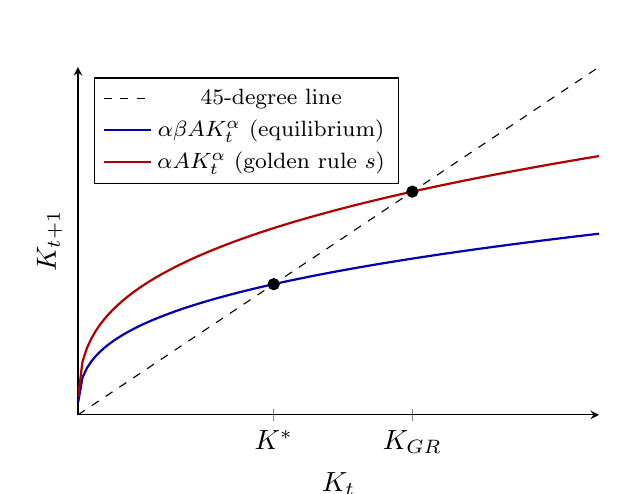
\begin{tikzpicture}
\begin{axis}[width=8.2cm,height=6cm,xmin=0,xmax=0.3,ymin=0,ymax=0.3,xlabel={$K_t$},ylabel={$K_{t+1}$},
  axis lines=left,xtick={0.1127,0.1925},xticklabels={$K^\ast$,$K_{GR}$},ytick=\empty,legend pos=north west,
  legend style={font=\footnotesize}]
\addplot[black,dashed,domain=0:0.3] {x}; \addlegendentry{45-degree line}
\addplot[blue!70!black,thick,domain=0.0001:0.3,samples=120] {(0.7/3)*x^(1/3)}; \addlegendentry{$\alpha\beta AK_t^\alpha$ (equilibrium)}
\addplot[red!70!black,thick,domain=0.0001:0.3,samples=120] {(1/3)*x^(1/3)}; \addlegendentry{$\alpha AK_t^\alpha$ (golden rule $s$)}
\addplot[only marks,mark=*] coordinates {(0.1127,0.1127) (0.1925,0.1925)};
\end{axis}
\end{tikzpicture}\\[-2pt]
{\footnotesize Drawn with $A=1$, $\alpha=1/3$, $\beta=0.7$: $K^\ast=(0.7/3)^{1.5}=0.113$, $K_{GR}=(1/3)^{1.5}=0.192$.}
\end{center}
\passo{Solow}{Solow with $\delta=1$, $n=0$ reads}
\begin{equation}
K_{t+1}=sAK_t^\alpha, \label{b6q18:solow}
\end{equation}
which is \eqref{b6q18:rK} with $s=\alpha\beta$. The difference is that $s$ is \emph{chosen}, from patience and the capital share.
\passo{golden rule}{In a steady state of \eqref{b6q18:solow}, consumption is output minus replacement:}
\begin{equation}
c=AK^\alpha-K. \label{b6q18:cGR}
\end{equation}
Maximize \eqref{b6q18:cGR} over $K$:
\begin{equation}
\alpha AK^{\alpha-1}=1. \label{b6q18:GRfoc}
\end{equation}
The saving rate that sustains it follows from \eqref{b6q18:solow} with $K_{t+1}=K_t$, then \eqref{b6q18:GRfoc}:
\begin{align*}
s_{GR}&=\frac{K}{AK^\alpha}=\frac{1}{AK^{\alpha-1}}\\
&=\frac{1}{(1/\alpha)}\\
&=\alpha>\alpha\beta .
\end{align*}
So $K^\ast<K_{GR}$. At $K^\ast$, \eqref{b6q18:Kstar} gives $\alpha A{K^\ast}^{\alpha-1}=\frac1\beta$: the modified golden rule
$F_K-\delta=\frac1\beta-1$ with $\delta=1$, not \eqref{b6q18:GRfoc}. The two-period economy of (b) saved $\frac{\alpha\beta}{1+\alpha\beta}<\alpha\beta$
\eqref{b6q18:s}: with a last period, capital has no use after it.
\intuicao{One household's Euler equation plus market clearing ($K_{t+1}$ = what it saves) is a Solow law of motion with an
endogenous saving rate. Efficiency (item (c)) and the golden rule answer different questions.}
\refbib{Kurlat (2020), \S9.3, pp.~172--179; \S4.3 (golden rule); Exercise 9.12, p.~185; Prova~01, Q2(e)--(f).}
\rubrica{
\item Euler verified line by line (1), transversality (0.5): 1.5 pts. \item Graph: axes labeled, map, 45-degree line, $K^\ast$ (0.5); stability (0.5).
\item Solow with $s=\alpha\beta$ chosen vs $s_{GR}=\alpha$: 0.5 pt. ``Equilibrium = golden rule'': 0 for this line. No graph: max.\ 2 pts.
}
\end{sol}

% =============================================================================
% Block 7 --- Aula 7: money and inflation (Kurlat chs. 10-11). Checks: practice-all-topics-check-b.py, Block 7.
% Solution format (rules/00_estilo_avaliacao.md §4): Notation list, numbered equations cited with \eqref,
% one operation per displayed line. Labels: b7q<question>:<name>.
\bloco{7}{Money and inflation: aggregates, money demand, the quantity theory, seigniorage}{Kurlat chs.~10--11 (Aula 7) \,\textbullet\, 25 points}

\questao{(5 points) Objective items.}

\textbf{a)} (3 points) A Brazilian saver holds a fixed-rate (\emph{prefixado}) bond. Income tax takes $\tau=15\%$ of the
\emph{nominal} interest. The real rate is $r=7\%$ and the Fisher effect holds ($i=r+\pi$). Anticipated inflation rises from
$5\%$ to $10\%$. The after-tax real return $(1-\tau)i-\pi$ goes:
\begin{alternativas}
\item from $5.95\%$ to $5.95\%$
\item from $5.2\%$ to $4.45\%$
\item from $7\%$ to $7\%$
\item from $12\%$ to $17\%$
\end{alternativas}
\gabarito{B}
\begin{sol}
\begin{notacao}
\item $i$: nominal rate; $r$: pre-tax real rate; $\pi$: anticipated inflation; $\tau\in(0,1)$: tax on nominal interest; $r^\tau$: after-tax real return.
\end{notacao}
\passo{computation}{The statement gives the Fisher relation and the after-tax real return:}
\begin{align}
i&=r+\pi, \label{b7q19:fisher}\\
r^\tau&=(1-\tau)i-\pi. \label{b7q19:ret}
\end{align}
Substituting \eqref{b7q19:fisher} into \eqref{b7q19:ret}:
\begin{align}
r^\tau&=(1-\tau)(r+\pi)-\pi\nonumber\\
&=(1-\tau)r-\tau\pi. \label{b7q19:ret2}
\end{align}
Before, by \eqref{b7q19:fisher} and then \eqref{b7q19:ret}; after, the same with $\pi=10$:
\begin{align*}
i&=7+5=12\%,\\
r^\tau&=(1-0.15)\times(12)-5\\
&=0.85\times12-5=10.2-5=5.2\%,\\
i&=7+10=17\%,\\
r^\tau&=(1-0.15)\times(17)-10\\
&=0.85\times17-10=14.45-10=4.45\%.
\end{align*}
By \eqref{b7q19:ret2}, the loss is $\tau\,\Delta\pi=0.15\times5=0.75$ points: the tax falls on the inflation premium, which is not income.
\passo{distractors}{A taxes only the real return, the first term of \eqref{b7q19:ret2}, $(1-\tau)r=0.85\times7=5.95\%$, as an indexed tax system would. C forgets the tax (the
Fisher effect alone keeps the pre-tax real rate at 7\%). D makes two mistakes: no tax and nominal instead of real returns.}
\refbib{Kurlat (2020), \S11.1 (Fisher equation) and \S11.4 (The Cost of Inflation), pp.~205--222.}
\end{sol}

\medskip
\textbf{b)} (2 points, T or F) With Baumol--Tobin money demand and flexible prices, a permanent, anticipated rise in the growth
rate of money raises inflation one for one in the new steady state and leaves real money balances unchanged.
\gabarito{F}
\begin{sol}
\begin{notacao}
\item $\mu$: money growth; $\pi$: inflation; $g$: real growth; $\eta$: income elasticity of money demand; $i$, $r$: nominal and
real rates; $M/P$: real balances; $F$: real cost of a bank trip; $Y$: real spending.
\end{notacao}
\passo{proof}{The first half is right: in a steady state}
\begin{equation}
\pi=\mu-\eta g, \label{b7q19:qt}
\end{equation}
with $g$ unchanged, so $d\pi=d\mu$. The second half is not. By Fisher, $i=r+\pi$, so $i$ rises one for one. Baumol--Tobin demand is
\begin{equation}
\frac MP=\sqrt{\frac{FY}{2i}}, \label{b7q19:bt}
\end{equation}
whose interest elasticity, from the log of \eqref{b7q19:bt}, is
\begin{equation}
\frac{\partial\ln(M/P)}{\partial\ln i}=-\frac12. \label{b7q19:el}
\end{equation}
By \eqref{b7q19:el}, real balances fall. Money is neutral in \emph{levels} but not superneutral:
a change in its \emph{growth rate} changes a real variable (and the resources spent on trips to the bank).
\refbib{Kurlat (2020), \S10.4 and \S11.2, pp.~199--215.}
\end{sol}

% -----------------------------------------------------------------------------
\questao{(8 points) \textit{Source: Kurlat, P. (2020), \emph{A Course in Modern Macroeconomics}, Exercise 11.6 ``Seignorage with High
Inflation'', pp.~219--221 --- reproduced verbatim; this list asks items (a)--(j) only (the book's items (k)--(u) are omitted).}}

\noindent Suppose that money demand is given by:
\[
m^D(Y_t,i_{t+1})=Y_t\cdot(1+i_{t+1})^{-\mu}
\]
where $\mu$ is a parameter. This is sometimes known as the Cagan money-demand function. Equilibrium in the money market is given by:
\[
M_t^S=Y_t\cdot(1+i_{t+1})^{-\mu}\,p_t
\]
The real economy is in a steady state so that:
\begin{align*}
Y_t&=Y_{ss}\\
r_{t+1}&=r_{ss}
\end{align*}
The government obtains seignorage revenue $S_t$ (in real terms) by expanding the monetary base. $S_t$ is given by:
\[
S_t=\frac{M_t^B-M_{t-1}^B}{P_t} \tag{11.4.2}
\]
Let $\omega$ be the money multiplier, so that $M^S=\omega M^B$.\par
\noindent Suppose that the rate of growth of the money supply is constant at rate $\gamma$, i.e.:
\[
M_t^S=(1+\gamma)\,M_{t-1}^S \tag{11.4.3}
\]
\begin{enumerate}[label=(\alph*),leftmargin=2.2em,topsep=2pt,itemsep=1pt]
\item What will be the rate of inflation?
\item What will be nominal interest rate?
\item Find an expression for the level of real money balances. How does it depend on $\gamma$? Why?
\item Solve equation (11.4.3) for $M_{t-1}^S$ and replace this in (11.4.2) to obtain an expression for seignorage revenue $S_t$ in terms
of $\gamma$ and $\frac{M_t^S}{P_t}$. How does $S_t$ depend on $\gamma$? How does it depend on $\frac{M_t^S}{P_t}$? Why?
\item Replace the value of $\frac{M_t^S}{P_t}$ that you found in part (c) into the expression for $S_t$ that you found in part (d) to
obtain an expression for seignorage revenues $S_t$ in terms of $\gamma$, $Y_{ss}$, $r_{ss}$, $\omega$ and $\mu$.
\item Assume the following parameter values:
\begin{align*}
Y_{ss}&=1\\
\mu&=4\\
r_{ss}&=0.0025\\
\omega&=5
\end{align*}
Note that $\mu=4$ is close to the value that has been empirically estimated in some high inflation countries when the time period
is one month. To be consistent, $r_{ss}$ should be interpreted as a monthly real interest rate and $Y_{ss}$ as monthly GDP.
\item Plot $S_t$ against $\gamma$ for values of $\gamma$ between 0 and 0.8.
\item What is the monthly rate of growth of the money supply that maximizes seignorage revenue? Call this $\gamma^*$.
\item Why is seignorage revenue decreasing in $\gamma$ for $\gamma>\gamma^*$?
\item What monthly inflation rate does $\gamma=\gamma^*$ imply?
\end{enumerate}
\noindent\textit{Added to the book's items (not in the book):} draw the plot of part (g). Careful with notation: here $\mu$ is the
Cagan semi-elasticity, not money growth ($\gamma$).
\resolespaco
\begin{sol}
\begin{notacao}
\item $M_t$: money (M1); $MB_t$: monetary base; $\omega>1$: money multiplier, $M_t=\omega MB_t$; $P_t$: price level.
\item $\gamma>0$: growth rate of money per month; $\pi$: inflation; $i$: nominal rate; $r_{ss}$: steady-state real rate.
\item $\mu>0$: Cagan semi-elasticity of money demand (\emph{not} money growth); $Y_{ss}$: steady-state real output.
\item $S_t$: real seignorage (revenue from issuing base money); $\gamma^\ast$: revenue-maximizing money growth.
\end{notacao}
\passo{(a) inflation}{In a steady state $Y_t=Y_{ss}$ and $r_{t+1}=r_{ss}$. Real money demand is}
\begin{equation}
\frac{M_t}{P_t}=Y_{ss}(1+i)^{-\mu}. \label{b7q20:md}
\end{equation}
If $\pi$ is constant, $i$ is constant, so by \eqref{b7q20:md} real balances are constant. Then prices grow with money:
\begin{equation}
\frac{P_t}{P_{t-1}}=\frac{M_t}{M_{t-1}}=1+\gamma, \label{b7q20:pi}
\end{equation}
so $\boxed{\pi=\gamma}$, consistent with the guess.
\passo{(b) nominal rate}{The exact Fisher equation is}
\begin{equation}
1+i=(1+r_{ss})(1+\pi). \label{b7q20:fisher}
\end{equation}
Using $\pi=\gamma$ from \eqref{b7q20:pi}:
\begin{equation}
1+i=(1+r_{ss})(1+\gamma), \label{b7q20:i}
\end{equation}
so $i=(1+r_{ss})(1+\gamma)-1\approx r_{ss}+\gamma$.
\passo{(c) real balances}{Substitute \eqref{b7q20:i} into \eqref{b7q20:md}:}
\begin{equation}
\frac{M_t}{P_t}=Y_{ss}\left[(1+r_{ss})(1+\gamma)\right]^{-\mu}, \label{b7q20:m}
\end{equation}
decreasing in $\gamma$: faster money growth means more inflation, a higher nominal rate and a higher cost of holding money, so
people hold less.
\passo{(d) seignorage}{The government issues only base money, and by \eqref{b7q20:pi} money grows at $\gamma$:}
\begin{align}
MB_t&=\frac{M_t}{\omega},\qquad M_{t-1}=\frac{M_t}{1+\gamma}, \label{b7q20:mb}\\
S_t&=\frac{MB_t-MB_{t-1}}{P_t}. \label{b7q20:Sdef}
\end{align}
Substitute \eqref{b7q20:mb} into \eqref{b7q20:Sdef}:
\begin{align}
S_t&=\frac{\big(\frac{M_t}{\omega}\big)-\big(\frac{M_t}{(1+\gamma)\,\omega}\big)}{P_t}\nonumber\\
&=\frac1\omega\,\frac{M_t-\frac{M_t}{1+\gamma}}{P_t}\nonumber\\
&=\frac{\gamma}{(1+\gamma)\,\omega}\,\frac{M_t}{P_t}. \label{b7q20:S}
\end{align}
Given $\frac MP$, $S$ rises with $\gamma$ (a higher tax rate) and is proportional to real balances (the tax base). It is divided by
$\omega$ because only base money is issued by the government; deposits created by banks are not its revenue.
\passo{(e) in parameters}{Substitute \eqref{b7q20:m} into \eqref{b7q20:S}:}
\begin{equation}
S=\frac{\gamma}{(1+\gamma)\,\omega}\,Y_{ss}\left[(1+r_{ss})(1+\gamma)\right]^{-\mu}. \label{b7q20:Sp}
\end{equation}
\passo{(f)--(g) plot}{With $Y_{ss}=1$, $\mu=4$, $r_{ss}=0.0025$, $\omega=5$, \eqref{b7q20:Sp} becomes}
\begin{align}
S(\gamma)&=\frac{\gamma}{(1+\gamma)\,(5)}\,(1)\left[(1+0.0025)(1+\gamma)\right]^{-(4)}\nonumber\\
&=\frac{\gamma}{5(1+\gamma)}\left[1.0025(1+\gamma)\right]^{-4}. \label{b7q20:Snum}
\end{align}
\begin{center}
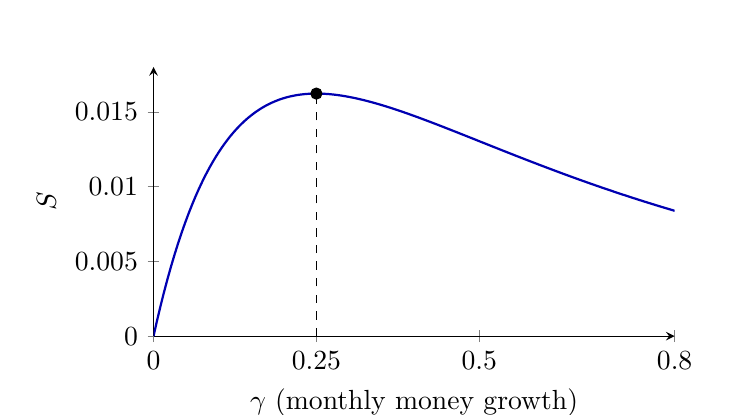
\begin{tikzpicture}
\begin{axis}[width=8.2cm,height=5cm,xmin=0,xmax=0.8,ymin=0,ymax=0.018,xlabel={$\gamma$ (monthly money growth)},ylabel={$S$},
  axis lines=left,scaled y ticks=false,yticklabel style={/pgf/number format/fixed,/pgf/number format/precision=3},
  xtick={0,0.25,0.5,0.8}]
\addplot[blue!70!black,thick,domain=0:0.8,samples=150] {x/(5*(1+x))*(1.0025*(1+x))^(-4)};
\addplot[dashed] coordinates {(0.25,0) (0.25,0.01622)};
\addplot[only marks,mark=*] coordinates {(0.25,0.01622)};
\end{axis}
\end{tikzpicture}
\end{center}
It rises from $0$, peaks at $\gamma=0.25$ ($S=0.0162$) and falls to $0.0084$ at $\gamma=0.8$: a Laffer curve.
\passo{(h) maximum}{Take the log of \eqref{b7q20:Sp}:}
\begin{equation}
\ln S=\ln\gamma-\ln(1+\gamma)-\ln\omega+\ln Y_{ss}-\mu\ln(1+r_{ss})-\mu\ln(1+\gamma). \label{b7q20:lnS}
\end{equation}
Differentiate \eqref{b7q20:lnS} with respect to $\gamma$:
\begin{align}
\frac{d\ln S}{d\gamma}&=\frac1\gamma-\frac{1}{1+\gamma}-\frac{\mu}{1+\gamma}\nonumber\\
&=\frac1\gamma-\frac{1+\mu}{1+\gamma}\nonumber\\
&=\frac{1-\mu\gamma}{\gamma(1+\gamma)}. \label{b7q20:dlnS}
\end{align}
\eqref{b7q20:dlnS} is zero at $\boxed{\gamma^\ast=1/\mu=0.25}$ per month; positive below, negative above, so it is the maximum.
Revenue there, from \eqref{b7q20:Snum}:
\begin{align*}
S^\ast&=\frac{0.25}{5(1+0.25)}\left[1.0025(1+0.25)\right]^{-4},\\
1.0025\times1.25&=1.253125,\\
1.253125^4&=2.4659,\\
S^\ast&=\frac{0.25}{5\times1.25}\cdot\frac1{2.4659}=\frac{0.04}{2.4659}=0.0162,
\end{align*}
about $1.6\%$ of monthly GDP, with real balances $1/2.4659=0.4055$ by \eqref{b7q20:m} and $i=25.3\%$ a month by \eqref{b7q20:i}.
\passo{(i) why it falls}{The first line of \eqref{b7q20:dlnS} adds the gain in the rate, $\frac1\gamma-\frac1{1+\gamma}=\frac1{\gamma(1+\gamma)}$, and the loss in the base, $-\frac{\mu}{1+\gamma}$.
For $\gamma>1/\mu$ the base shrinks faster than the rate rises: people economize so much on money that more inflation collects less.}
\passo{(j) inflation}{By \eqref{b7q20:pi}, $\pi=\gamma^\ast=25\%$ a month, i.e.\ $1.25^{12}-1=13.55$, about $1{,}355\%$ a year: a high-inflation regime of the
kind Brazil lived through before the Plano Real.}
\intuicao{Seignorage is a tax whose base is the public's real balances; the base responds to the rate through the Cagan
semi-elasticity $\mu$, so the revenue-maximizing money growth is $1/\mu$, and governments that print faster collect less.}
\refbib{Kurlat (2020), \S11.3 (Seignorage), eq.~(11.4.2), pp.~215--218; Exercise 11.6, pp.~219--220. Same result
($\pi^{\max}=1/a$ in the continuous Cagan form) in the project's Map notes (Aula 7, note 04, \S4.2). No instructor key covers 11.6.}
\rubrica{
\item (a)--(c) 2 pts; (d)--(e) 2 pts; (f)--(g) plot with labeled axes and the peak marked 1 pt; (h) 2 pts (FOC 1, $\gamma^\ast$ and $S^\ast$ 1); (i)--(j) 1 pt.
\item Seignorage written as $\pi\frac MP$ without the base/multiplier step: max.\ 1 pt in (d)--(e). Treating more money growth as always more revenue: 0 in (i).
}
\end{sol}

% -----------------------------------------------------------------------------
\questao{(12 points) Discursive. \emph{From the monetary base to the price level: a credible disinflation.} The Banco Central do
Brasil (BCB) controls the base $B$. The public holds currency and deposits in the ratio $c=C/D=0.25$; banks hold reserves (required
plus excess) in the ratio $\theta=R/D=0.20$. Real money demand follows Baumol--Tobin: spending $Y$ per period is withdrawn in
$N$ equal trips to the bank, each costing $F$ in real terms. Prices are flexible, real output grows at $g=2\%$, the real rate is
constant at $r=4\%$ and M1 grows at $\mu=6\%$ (illustrative values).}

\textbf{a)} (3 points) Derive the money multiplier $m=M1/B$ and compute it. The BCB cuts reserve requirements so that $\theta$ falls to
$0.15$: by how much does M1 change for a given base? Why is $m$ not a constant the BCB can rely on?
\resolespaco
\begin{sol}
\begin{notacao}
\item $B$: monetary base; $C$: currency held by the public; $D$: deposits; $R$: bank reserves; $M1$: currency plus deposits.
\item $c=C/D>0$: currency-deposit ratio; $\theta=R/D\in(0,1)$: reserve ratio; $m=M1/B$: money multiplier.
\end{notacao}
\passo{derivation}{The two identities are}
\begin{align}
B&=C+R, \label{b7q21:B}\\
M1&=C+D. \label{b7q21:M1}
\end{align}
Divide \eqref{b7q21:B} and \eqref{b7q21:M1} by $D$:
\begin{align}
\frac BD&=c+\theta, \label{b7q21:BD}\\
\frac{M1}D&=1+c. \label{b7q21:MD}
\end{align}
Divide \eqref{b7q21:MD} by \eqref{b7q21:BD}:
\begin{equation}
m=\frac{M1}{B}=\frac{1+c}{c+\theta}. \label{b7q21:m}
\end{equation}
\passo{numbers}{From \eqref{b7q21:m}:}
\begin{align*}
m_0&=\frac{1+0.25}{0.25+0.20}\\
&=\frac{1.25}{0.45}=2.778,\\
m_1&=\frac{1+0.25}{0.25+0.15}\\
&=\frac{1.25}{0.40}=3.125,\\
\frac{m_1}{m_0}&=\frac{(1.25/0.40)}{(1.25/0.45)}\\
&=\frac{0.45}{0.40}=1.125 .
\end{align*}
M1 rises by $12.5\%$ with the same base; differentiating \eqref{b7q21:m}, $\partial m/\partial\theta=-\frac{1+c}{(c+\theta)^2}<0$.
\passo{caveat}{\eqref{b7q21:m} is an identity in two behavioral ratios. Banks choose excess reserves and the public chooses $c$; in a crisis both rise
and $m$ collapses (as in 2008), so a given base does not pin down M1.}
\rubrica{\item Derivation 1 pt; numbers 1 pt; why $m$ moves 1 pt.}
\end{sol}

\textbf{b)} (3 points) Derive Baumol--Tobin money demand, its income and interest elasticities, and the implied velocity.
\resolespaco
\begin{sol}
\begin{notacao}
\item $Y>0$: real spending per period; $N>0$: trips to the bank per period; $F>0$: real cost of a trip; $i>0$: nominal rate.
\item $\mathcal C(N)$: total cost of managing cash; $\ell\equiv M/P$: real money balances; $V$: velocity; $P$: price level.
\end{notacao}
\passo{problem}{With $N$ trips, cash falls from $Y/N$ to 0 between trips, so average real balances are}
\begin{equation}
\ell=\frac{Y}{2N}. \label{b7q21:avg}
\end{equation}
The total cost is trips plus the interest forgone on \eqref{b7q21:avg}:
\begin{equation}
\mathcal C(N)=FN+i\,\frac{Y}{2N}. \label{b7q21:cost}
\end{equation}
Differentiate \eqref{b7q21:cost} and set it to zero:
\begin{equation}
F-\frac{iY}{2N^2}=0. \label{b7q21:foc}
\end{equation}
Solve \eqref{b7q21:foc} for $N$ (the second derivative is $\frac{iY}{N^3}>0$, so it is a minimum):
\begin{equation}
N^\ast=\sqrt{\frac{iY}{2F}}. \label{b7q21:N}
\end{equation}
\passo{demand}{Substitute \eqref{b7q21:N} into \eqref{b7q21:avg}:}
\begin{align}
\ell&=\frac{Y}{2\Big(\sqrt{\frac{iY}{2F}}\Big)}\nonumber\\
&=\frac Y2\sqrt{\frac{2F}{iY}}\nonumber\\
&=\sqrt{\frac{FY}{2i}}. \label{b7q21:bt}
\end{align}
Taking logs of \eqref{b7q21:bt}, $\ln\ell=\frac12(\ln F+\ln Y-\ln2-\ln i)$, so
\[
\frac{\partial\ln\ell}{\partial\ln Y}=\frac12,\qquad \frac{\partial\ln\ell}{\partial\ln i}=-\frac12 .
\]
\passo{velocity}{The quantity equation is}
\begin{equation}
MV=PY. \label{b7q21:qt}
\end{equation}
Solve \eqref{b7q21:qt} for $V$ and use \eqref{b7q21:bt}:
\begin{align}
V&=\frac{Y}{\ell}=\frac{Y}{\sqrt{FY/(2i)}}\nonumber\\
&=\sqrt{\frac{2iY}{F}}. \label{b7q21:V}
\end{align}
It rises with $i$ and $Y$ and falls with $F$. So $V$ is not a constant and \eqref{b7q21:qt}, an identity, becomes a theory only once
$V$ is pinned down by a money-demand function.
\rubrica{\item Cost function and FOC: 1 pt. \item Demand and both elasticities: 1 pt. \item Velocity and the identity remark: 1 pt.}
\end{sol}

\textbf{c)} (3 points) In a steady state with constant $i$, show that $\pi=\mu-\eta g$, where $\eta$ is the income elasticity of money
demand. Compute $\pi$ and $i$ (exact Fisher) now, and the money growth the BCB needs for an inflation target of $3\%$.
\resolespaco
\begin{sol}
\begin{notacao}
\item $M$: M1; $\ell^D(Y,i)$: real money demand; $\mu=\dot M/M$: growth of M1; $\pi=\dot P/P$: inflation; $g=\dot Y/Y$: real growth.
\item $\eta\equiv\frac{\partial\ell^D}{\partial Y}\frac{Y}{\ell^D}$: income elasticity of money demand; $r$: real rate; $i$: nominal rate.
\end{notacao}
\passo{derivation}{In equilibrium money supply equals money demand:}
\begin{equation}
M=P\,\ell^D(Y,i). \label{b7q21:eq}
\end{equation}
Log-differentiate \eqref{b7q21:eq} in time, with $\dot i=0$:
\begin{equation}
\frac{\dot M}M=\frac{\dot P}P+\frac{\partial\ell^D}{\partial Y}\frac{Y}{\ell^D}\frac{\dot Y}Y. \label{b7q21:logd}
\end{equation}
In the notation above, \eqref{b7q21:logd} reads $\mu=\pi+\eta g$, so
\begin{equation}
\pi=\mu-\eta g. \label{b7q21:pi}
\end{equation}
Baumol--Tobin \eqref{b7q21:bt} gives $\eta=\frac12$.
\passo{numbers}{By \eqref{b7q21:pi}, $\pi_0=6-\frac12\times2=5\%$. The exact Fisher equation is}
\begin{equation}
1+i=(1+r)(1+\pi). \label{b7q21:fisher}
\end{equation}
By \eqref{b7q21:fisher}, $1+i_0=1.04\times1.05=1.092$, so $i_0=9.2\%$ (approximate: $9\%$). For the target $\pi_1=3\%$, solve \eqref{b7q21:pi} for $\mu$:
\begin{align*}
\mu_1&=\pi_1+\eta g\\
&=3+\tfrac12\times2=4\%,\\
1+i_1&=1.04\times1.03=1.0712,\quad i_1=7.12\%.
\end{align*}
\refbib{Instructor's key, PSET~6 Q2(a)--(b) (Lista~6): same derivation and $\eta=\tfrac12$, $\mu=3.5\%$ for a $2\%$ target with $g=3\%$.}
\rubrica{\item Derivation with $\dot i=0$ stated: 1.5 pts. \item Numbers: 1.5 pts. Using $\pi=\mu-g$ ($\eta=1$) for Baumol--Tobin: max.\ 1 pt.}
\end{sol}

\textbf{d)} (3 points) At date $T$ the BCB announces, credibly, that M1 will grow at $4\%$ from now on; $M_T$ itself does not change.
What happens to the price level at $T$ and afterwards? Draw $\ln P_t$. Is money superneutral here? What one-off operation would
avoid any jump in $P$?
\resolespaco
\begin{sol}
\begin{notacao}
\item $T$: announcement date; $M_T$: M1 at $T$ (given); $P_T$: price level at $T$.
\item $\ell_0,\ell_1$: desired real balances under the old ($i_0$) and new ($i_1$) steady states, at the same $Y_T$, $F$.
\end{notacao}
\passo{real balances}{By \eqref{b7q21:bt}, with $F$ and $Y_T$ the same in both regimes, desired balances scale with $i^{-1/2}$. Using $i_0$, $i_1$ from (c):}
\begin{align}
\frac{\ell_1}{\ell_0}&=\frac{\big(\sqrt{FY_T/(2i_1)}\big)}{\big(\sqrt{FY_T/(2i_0)}\big)}\nonumber\\
&=\sqrt{\frac{i_0}{i_1}} \label{b7q21:ratio}\\
&=\sqrt{\frac{0.092}{0.0712}}=\sqrt{1.2921}=1.1367.\nonumber
\end{align}
\passo{the jump}{The money market clears at $T$ with $M_T$ given, so by \eqref{b7q21:eq}}
\begin{equation}
P_T=\frac{M_T}{\ell}. \label{b7q21:PT}
\end{equation}
Dividing \eqref{b7q21:PT} under the new and old demand, then using \eqref{b7q21:ratio}:
\begin{align*}
\frac{P_T^{\text{new}}}{P_T^{\text{old}}}&=\frac{(M_T/\ell_1)}{(M_T/\ell_0)}\\
&=\frac{\ell_0}{\ell_1}=\frac1{(1.1367)}.
\end{align*}
$P$ falls by $12.0\%$ at $T$ ($\Delta\ln P=-\frac12\ln1.2921=-0.128$), then by \eqref{b7q21:pi} grows at $3\%$ instead of $5\%$.
\begin{center}
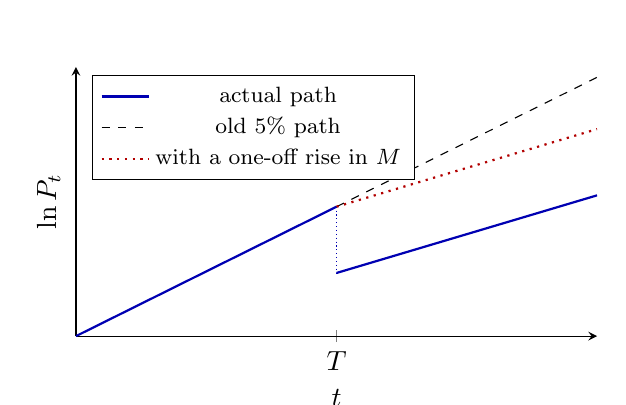
\begin{tikzpicture}
\begin{axis}[width=8.2cm,height=5cm,xmin=0,xmax=10,ymin=0,ymax=0.52,xlabel={$t$},ylabel={$\ln P_t$},axis lines=left,
  xtick={5},xticklabels={$T$},ytick=\empty,legend pos=north west,legend style={font=\footnotesize}]
\addplot[blue!70!black,thick] coordinates {(0,0) (5,0.25)}; \addlegendentry{actual path}
\addplot[black,dashed] coordinates {(5,0.25) (10,0.5)}; \addlegendentry{old $5\%$ path}
\addplot[red!70!black,dotted,thick] coordinates {(5,0.25) (10,0.40)}; \addlegendentry{with a one-off rise in $M$}
\addplot[blue!70!black,thick,forget plot] coordinates {(5,0.122) (10,0.272)};
\addplot[blue!70!black,densely dotted,forget plot] coordinates {(5,0.25) (5,0.122)};
\end{axis}
\end{tikzpicture}
\end{center}
\passo{superneutrality}{No: by \eqref{b7q21:ratio}, a change in money \emph{growth} changed real balances by $13.7\%$ (and the resources spent on bank trips).
Money is neutral only in \emph{levels}.}
\passo{avoiding the jump}{By \eqref{b7q21:PT}, $P_T$ is unchanged if $M_T$ rises in the same proportion as $\ell$. So raise $M$ once at $T$ by $13.7\%$
(buy bonds, expanding the base) and let it grow at $4\%$ afterwards: the public's higher demand for real balances is met by more
money instead of a lower $P$ (the remonetization seen in Brazil after the Plano Real).}
\intuicao{Lower expected inflation lowers the cost of holding money, so the public wants more of it at once; with $M$ fixed the only
way to supply real balances is a fall in $P$.}
\refbib{Kurlat (2020), \S11.2 (steady states with money growth), pp.~208--215; project Map notes (Aula 7, note 03, \S3.6).}
\rubrica{\item Ratio of real balances 1 pt. \item Jump with sign and size, graph with axes and slopes: 1 pt (graph alone 0.5).
\item Superneutrality and the one-off injection: 1 pt. A jump \emph{up} in $P$: max.\ 1 pt in the item.}
\end{sol}

% =============================================================================
% Block 8 --- Aula 8: AS-AD microfoundations (Benigno 2015, sections 1-5). Checks: practice-all-topics-check-b.py, Block 8.
% Solution format (rules/00_estilo_avaliacao.md §4): Notation list, numbered equations cited with \eqref,
% one operation per displayed line. Labels: b8:AD, b8:AS (notation paragraph), b8q<question>:<name>.
\bloco{8}{The New Keynesian AS--AD model: microfoundations}{Benigno (2015) \S\S1--5 (Aula 8) \,\textbullet\, 25 points}

{\footnotesize\noindent\textbf{Notation for Blocks 8--9 (Benigno 2015).} Lower-case letters are log deviations from an efficient
steady state; bars denote the long run. Households: $u(C)-v(L)+\beta\{u(\bar C)-v(\bar L)\}$, $u_c=C^{-1/\tilde\sigma}$, $v=L^{1+\eta}/(1+\eta)$,
$\rho\equiv-\ln\beta$; resources $y=s_cc+g$, $\sigma\equiv\tilde\sigma s_c$. Firms: technology $Y(j)=AL(j)$, desired markup $\mu$ (monopoly power and
taxes, $\mu\simeq\mu_\theta+\tau+\tau_c$, with $\tau$ collecting labor, payroll and sales taxes); a fraction $\alpha$ of prices is preset at $p^e$.
AD, Benigno's eq.~(21), and AS, eq.~(20), with $\kappa=\frac{(1-\alpha)(\sigma^{-1}+\eta)}{\alpha}$:
\begin{align}
y&=\bar y_n+(g-\bar g)-\sigma[i-(\bar p-p)-(\bar\tau_c-\tau_c)-\rho], \tag{AD}\label{b8:AD}\\
p-p^e&=\kappa(y-y_n). \tag{AS}\label{b8:AS}
\end{align}
Calibration when numbers are asked (Benigno, p.~515): $\alpha=0.66$, $\sigma=0.5$, $\eta=0.2$, so $\sigma^{-1}+\eta=2.2$, $\kappa=1.133$.\par}

\questao{(5 points) Objective items.}

\textbf{a)} (3 points) Why does Benigno's AD curve slope downward in the $(y,p)$ plane?
\begin{alternativas}
\item A higher $p$ lowers real balances $M/P$, so the interest rate that clears the money market rises and spending falls.
\item A higher $p$, given $\bar p$, raises expected inflation $\bar p-p$, which lowers the real rate and pushes households to consume.
\item A higher $p$ lowers real balances, so the central bank's money-supply rule raises $i$ and households save more today.
\item A higher $p$, given $i$ and $\bar p$, lowers expected inflation $\bar p-p$, so the real rate rises and households save more.
\end{alternativas}
\gabarito{D}
\begin{sol}
\begin{notacao}
\item $y$, $p$: output and price level; $\bar p$: long-run price level; $i$: nominal rate; $i-(\bar p-p)$: real rate; $\sigma>0$.
\end{notacao}
\passo{key}{Differentiating \eqref{b8:AD} with $i$ and $\bar p$ fixed:}
\begin{equation}
\frac{\partial y}{\partial p}=-\sigma. \label{b8q22:slope}
\end{equation}
$p\uparrow$ means $\bar p-p\downarrow$, so the real rate $i-(\bar p-p)$ rises and the Euler equation moves consumption from today to
tomorrow. The channel is intertemporal; there is no LM curve, because the instrument is $i$.
\passo{distractors}{A is the IS--LM (Keynes-effect) story. B gets the sign of $\bar p-p$ wrong, which would reverse the sign of
\eqref{b8q22:slope} and make the curve slope upward. C makes two mistakes: the money-market channel and a money-supply instrument the model does not have.}
\refbib{Benigno (2015), \S3, eqs.~(1)--(6), pp.~505--506, and \S5, eq.~(21), p.~509.}
\end{sol}

\medskip
\textbf{b)} (2 points, T or F) News that the long-run desired markup $\bar\mu$ will be higher (current $\mu$ unchanged) shifts the AS curve
up today, because firms that reset prices raise them in anticipation.
\gabarito{F}
\begin{sol}
\begin{notacao}
\item $y_n$, $\bar y_n$: natural output today and in the long run; $a$, $g$, $\mu$ and $\bar a$, $\bar g$, $\bar\mu$: productivity, spending and markup today and in the long run.
\end{notacao}
\passo{proof}{\eqref{b8:AS} depends on $p^e$ and on current natural output, Benigno's eq.~(15), which contains the current $\mu$ only:}
\begin{equation}
y_n=\frac{(1+\eta)a+\sigma^{-1}g-\mu}{\sigma^{-1}+\eta}. \label{b8q22:yn}
\end{equation}
$\bar\mu$ enters the long-run version of \eqref{b8q22:yn},
\begin{equation}
\bar y_n=\frac{(1+\eta)\bar a+\sigma^{-1}\bar g-\bar\mu}{\sigma^{-1}+\eta}, \label{b8q22:ybn}
\end{equation}
which is in \eqref{b8:AD}. Differentiating \eqref{b8q22:ybn}, $d\bar y_n=-\frac{d\bar\mu}{\sigma^{-1}+\eta}$: lower expected permanent income cuts
consumption today, so the \emph{AD} shifts left by $\frac{d\bar\mu}{\sigma^{-1}+\eta}$. Rule: barred variables move the AD; current markups and
productivity move the AS.
\refbib{Benigno (2015), \S4, eq.~(15), and \S5, eq.~(21), pp.~507--509; Prova~01, Q3(a).}
\end{sol}

% -----------------------------------------------------------------------------
\questao{(8 points) \textit{Source: built on Benigno, P. (2015), ``New-Keynesian Economics: An AS--AD View'', \S4.1--\S4.4,
pp.~507--509 --- the article has no exercises; the statement below is ours.}
Natural versus efficient output: Benigno's eqs.~(14)--(15) and (19), the topic of Lista~7 Q3. Set $g=0$.}

\noindent What the article states (p.~509): ``A comparison of (19) with (15) shows that productivity and public spending shift the two
definitions of output in equal proportion. Mark-up shocks, however, are a source of inefficiencies, as they shift the natural but not
the efficient level of output.''

\textbf{a)} (3 points) Derive natural output $y_n$ (flexible prices) and efficient output $y_e$ (planner), and the gap between them.
\resolespaco
\begin{sol}
\begin{notacao}
\item $P$, $W$: price and nominal wage; $w-p$: log real wage; $A$, $a=\ln A$: productivity; $\mu\ge0$: desired markup.
\item $L$, $l$: hours and their log; $C$, $c$: consumption and its log; $y$: log output; $g=0$.
\item $\eta>0$: inverse Frisch elasticity; $\tilde\sigma>0$: intertemporal elasticity; $\sigma=\tilde\sigma s_c$; $u_c$, $v_l$: marginal utility of consumption and disutility of work.
\item $y_n$: natural output (flexible prices, with the markup); $y_e$: efficient output (planner, no markup).
\end{notacao}
\passo{natural}{A flexible firm sets its price as a markup over marginal cost $W/A$:}
\begin{equation}
P=(1+\mu)\frac WA. \label{b8q23:price}
\end{equation}
In logs, with $\ln(1+\mu)\simeq\mu$, \eqref{b8q23:price} gives the real wage firms pay:
\begin{equation}
w-p=a-\mu. \label{b8q23:ld}
\end{equation}
Labor supply equates the marginal rate of substitution to the real wage:
\begin{equation}
\frac{v_l(L)}{u_c(C)}=\frac WP. \label{b8q23:ls}
\end{equation}
In logs, \eqref{b8q23:ls} is
\begin{equation}
w-p=\eta l+\tilde\sigma^{-1}c. \label{b8q23:lsl}
\end{equation}
Technology and resources give
\begin{equation}
l=y-a,\qquad \tilde\sigma^{-1}c=\sigma^{-1}(y-g)=\sigma^{-1}y. \label{b8q23:tech}
\end{equation}
Substitute \eqref{b8q23:tech} into \eqref{b8q23:lsl} and equate with \eqref{b8q23:ld}:
\begin{align}
\eta\,(y-a)+\big(\sigma^{-1}y\big)&=(a-\mu)\nonumber\\
(\sigma^{-1}+\eta)\,y&=(1+\eta)a-\mu\nonumber\\
y_n&=\frac{(1+\eta)a-\mu}{\sigma^{-1}+\eta}. \label{b8q23:yn}
\end{align}
\passo{efficient}{The planner solves}
\begin{equation}
\max_Y\ u(Y)-v(Y/A). \label{b8q23:plan}
\end{equation}
The first-order condition of \eqref{b8q23:plan} is
\begin{equation}
u_c=\frac{v_l}{A},\quad\text{i.e.}\quad \mathrm{MRS}=\frac{v_l}{u_c}=A, \label{b8q23:pfoc}
\end{equation}
the marginal product of labor. In logs, using \eqref{b8q23:tech}, \eqref{b8q23:pfoc} is the first line of \eqref{b8q23:yn} with $\mu=0$:
\begin{align}
\eta\,(y-a)+\big(\sigma^{-1}y\big)&=a-(0)\nonumber\\
\eta(y-a)+\sigma^{-1}y&=a\nonumber\\
y_e&=\frac{(1+\eta)a}{\sigma^{-1}+\eta}. \label{b8q23:ye}
\end{align}
\passo{gap}{Subtract \eqref{b8q23:ye} from \eqref{b8q23:yn}:}
\begin{align}
y_n-y_e&=\Big(\frac{(1+\eta)a-\mu}{\sigma^{-1}+\eta}\Big)-\Big(\frac{(1+\eta)a}{\sigma^{-1}+\eta}\Big)\nonumber\\
&=-\frac{\mu}{\sigma^{-1}+\eta}<0. \label{b8q23:gap}
\end{align}
The markup is a wedge between the real wage firms pay ($A/(1+\mu)$, by \eqref{b8q23:price}) and the marginal product ($A$), so the
market works too little.
\rubrica{\item $y_n$ derived: 1.5 pts; $y_e$ derived: 1 pt; gap: 0.5 pt. Formulas quoted without derivation: max.\ 1 pt.}
\end{sol}

\textbf{b)} (3 points) Draw the labor market in the plane (hours $l$, real wage $w-p$) with $a=0$, marking natural and efficient
hours, and shade the welfare loss. Compute $y_n-y_e$ and the loss for $\mu=5\%$ at the calibration.
\resolespaco
\begin{sol}
\begin{notacao}
\item Symbols as in (a); $l_n$, $l_e$: natural and efficient hours (logs), with $a=0$.
\end{notacao}
\passo{graph}{With $a=0$, \eqref{b8q23:tech} gives $y=l$, so labor supply \eqref{b8q23:lsl} becomes}
\begin{align}
w-p&=\eta\,(l)+\sigma^{-1}(l)\nonumber\\
&=(\sigma^{-1}+\eta)\,l, \label{b8q23:sup}
\end{align}
with slope 2.2. The planner's line is $w-p=0$ (the marginal product); the market's line is $w-p=-\mu$, by \eqref{b8q23:ld}.
Setting \eqref{b8q23:sup} equal to each line:
\begin{align}
(\sigma^{-1}+\eta)\,l_n&=(-\mu),\qquad (\sigma^{-1}+\eta)\,l_e=(0),\nonumber\\
l_n&=-\frac{\mu}{\sigma^{-1}+\eta},\qquad l_e=0. \label{b8q23:ln}
\end{align}
\begin{center}
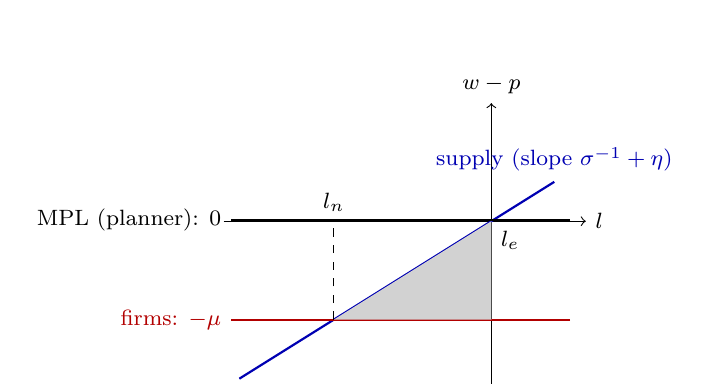
\begin{tikzpicture}[scale=1]
\draw[->] (-3.4,0) -- (1.2,0) node[right] {\footnotesize $l$};
\draw[->] (0,-2.2) -- (0,1.5) node[above] {\footnotesize $w-p$};
\draw[thick,blue!70!black] (-3.2,-2.0) -- (0.8,0.5) node[above] {\footnotesize supply (slope $\sigma^{-1}+\eta$)};
\draw[thick,red!70!black] (1.0,-1.25) -- (-3.3,-1.25) node[left] {\footnotesize firms: $-\mu$};
\draw[thick,black] (1.0,0.02) -- (-3.3,0.02) node[left] {\footnotesize MPL (planner): $0$};
\fill[gray!35] (-2.0,-1.25) -- (0,0) -- (0,-1.25) -- cycle;
\draw[dashed] (-2.0,-1.25) -- (-2.0,0) node[above] {\footnotesize $l_n$};
\node[below right] at (0,0) {\footnotesize $l_e$};
\end{tikzpicture}
\end{center}
\passo{numbers}{With $a=0$, $y=l$, so by \eqref{b8q23:ln}}
\begin{align*}
y_n-y_e&=l_n-l_e\\
&=\Big(-\frac{0.05}{2.2}\Big)-(0)\\
&=-2.27\%,
\end{align*}
as \eqref{b8q23:gap} also gives. The shaded triangle is the surplus lost on the hours not worked: its height is the wedge $\mu$
and its base is $l_e-l_n$ from \eqref{b8q23:ln}, so
\begin{align*}
\text{loss}&=\tfrac12\cdot\mu\cdot\frac{\mu}{\sigma^{-1}+\eta}\\
&=\tfrac12\cdot(0.05)\cdot\frac{(0.05)}{(2.2)}\\
&=\frac{0.05^2}{2\times2.2}=0.057\%\ \text{of output}.
\end{align*}
\refbib{Confirmed against the Lista~7 answer in \emph{Map}, \texttt{lista-07.md} ($-2.27\%$, $0.057\%$) and the instructor's key, PSET~7 Q4 ($y_n$ under flexible prices; $y_e$ removes market power).}
\rubrica{\item Graph: axes labeled, supply, the two horizontal lines, $l_n<l_e$: 1.5 pts. \item Numbers: 1.5 pts (gap 1, triangle 0.5).}
\end{sol}

\textbf{c)} (2 points) Which of $\alpha$, $\theta$, $a$, $g$ and the tax rates move $y_n-y_e$? Can monetary policy close it? What could?
\resolespaco
\begin{sol}
\begin{notacao}
\item $\theta>1$: elasticity of substitution between goods; $\mu_\theta=\ln\frac\theta{\theta-1}$: markup from monopoly power; $\alpha$: share of preset prices.
\end{notacao}
\passo{answer}{By \eqref{b8q23:gap}, only $\mu$ moves it: $\theta$ (via $\mu_\theta$) and the taxes in $\mu$. Productivity and spending move $y_n$ and $y_e$ by the
same amount (\eqref{b8q23:yn} and \eqref{b8q23:ye} have the same $a$ coefficient); stickiness $\alpha$ is in neither (they are flexible-price objects).
Monetary policy moves $y$ along \eqref{b8:AS}, not $y_n$, so it can make $y=y_e$ only by holding $p\neq p^e$. Closing the wedge itself
takes a real instrument: a production subsidy, financed lump sum, that offsets the markup (or lower distorting taxes).}
\rubrica{\item Correct list with the reason: 1 pt. \item Monetary vs fiscal instrument: 1 pt. ``Stickiness causes $y_n<y_e$'': 0 in the item.}
\end{sol}

% -----------------------------------------------------------------------------
\questao{(12 points) Discursive. \emph{Brazil's consumption-tax reform in the AS--AD model.} The reform replaces several taxes with
a value-added tax that phases in over years. Treat each fiscal change below as a deviation from an efficient steady state with
$p^e=\bar p=0$, $g=\bar g=0$ and $i=\rho$.}

\textbf{a)} (4 points) The household's budget is $(1+\tau_c)PC+\frac{(1+\bar\tau_c)\bar P\bar C}{1+i}=WL+\frac{\bar W\bar L}{1+i}+T$. Derive the Euler equation,
log-linearize it, and use $y=s_cc+g$ and long-run price flexibility to obtain the AD (21). Give its slope and explain it.
\resolespaco
\begin{sol}
\begin{notacao}
\item $C$, $\bar C$: consumption today and in the long run; $P$, $\bar P$: prices; $W$, $\bar W$, $L$, $\bar L$: wages and hours; $T$: lump-sum transfers.
\item $\tau_c$, $\bar\tau_c$: consumption-tax rates today and in the long run; $i$: nominal rate; $\lambda>0$: multiplier on the budget.
\item $\tilde\sigma>0$: intertemporal elasticity; $\rho=-\ln\beta$; $s_c\in(0,1]$: consumption share of output; $\sigma=\tilde\sigma s_c$.
\item Lower case ($c$, $\bar c$, $p$, $\bar p$, $y$, $g$): log deviations; $\bar y_n$: long-run natural output.
\end{notacao}
\passo{FOCs}{The budget of the statement is}
\begin{equation}
(1+\tau_c)PC+\frac{(1+\bar\tau_c)\bar P\bar C}{1+i}=WL+\frac{\bar W\bar L}{1+i}+T. \label{b8q24:bc}
\end{equation}
The Lagrangian with \eqref{b8q24:bc} is
\begin{multline}
\mathcal L=u(C)-v(L)+\beta\{u(\bar C)-v(\bar L)\}\\
+\lambda\Big[WL+\frac{\bar W\bar L}{1+i}+T-(1+\tau_c)PC-\frac{(1+\bar\tau_c)\bar P\bar C}{1+i}\Big]. \label{b8q24:lag}
\end{multline}
Differentiating \eqref{b8q24:lag} with respect to $C$ and $\bar C$:
\begin{align}
u_c(C)&=\lambda(1+\tau_c)P, \label{b8q24:fC}\\
\beta u_c(\bar C)&=\lambda\frac{(1+\bar\tau_c)\bar P}{1+i}. \label{b8q24:fCb}
\end{align}
Divide \eqref{b8q24:fC} by \eqref{b8q24:fCb}:
\begin{equation}
\frac{u_c(C)}{\beta u_c(\bar C)}=(1+i)\frac{(1+\tau_c)P}{(1+\bar\tau_c)\bar P}. \label{b8q24:euler}
\end{equation}
\passo{logs}{Take logs of \eqref{b8q24:euler} with $u_c=C^{-1/\tilde\sigma}$, $\ln\beta=-\rho$ and $\ln(1+x)\simeq x$:}
\begin{equation}
-\tilde\sigma^{-1}c+\tilde\sigma^{-1}\bar c+\rho=i+\tau_c-\bar\tau_c+p-\bar p. \label{b8q24:logeu}
\end{equation}
Multiply \eqref{b8q24:logeu} by $\tilde\sigma$ and rearrange:
\begin{equation}
\bar c-c=\tilde\sigma[i-(\bar p-p)-(\bar\tau_c-\tau_c)-\rho]. \label{b8q24:cc}
\end{equation}
\passo{AD}{From $y=s_cc+g$ in both periods,}
\begin{equation}
s_c(\bar c-c)=(\bar y-\bar g)-(y-g). \label{b8q24:res}
\end{equation}
Multiply \eqref{b8q24:cc} by $s_c$, use \eqref{b8q24:res} and $\sigma=\tilde\sigma s_c$:
\begin{align*}
s_c(\bar c-c)&=s_c\tilde\sigma[i-(\bar p-p)-(\bar\tau_c-\tau_c)-\rho]\\
\big((\bar y-\bar g)-(y-g)\big)&=(\sigma)[i-(\bar p-p)-(\bar\tau_c-\tau_c)-\rho].
\end{align*}
Long-run prices are flexible, so $\bar y=\bar y_n$. Substituting it and solving for $y$ gives \eqref{b8:AD}:
\begin{align*}
\big((\bar y_n)-\bar g\big)-(y-g)&=\sigma[i-(\bar p-p)-(\bar\tau_c-\tau_c)-\rho]\\
y&=\bar y_n+(g-\bar g)-\sigma[i-(\bar p-p)-(\bar\tau_c-\tau_c)-\rho].
\end{align*}
Slope $dp/dy=-1/\sigma$, the inverse of \eqref{b8q22:slope}: a higher $p$ lowers $\bar p-p$, raises the real rate and shifts consumption to the future.
\rubrica{\item FOCs and their ratio: 1.5 pts. \item Log-linear Euler: 1.5 pts. \item AD with slope and mechanism: 1 pt (money-demand story: 0 for this line).}
\end{sol}

\textbf{b)} (4 points) For each change, say which curve(s) move, in which direction, and by how much horizontally:
(i) a temporary rise in payroll tax, $d\tau>0$; (ii) an announced long-run rise, $d\bar\tau>0$; (iii) an announced long-run rise in the
consumption tax, $d\bar\tau_c>0$; (iv) a temporary rise in the consumption tax, $d\tau_c>0$.
\resolespaco
\begin{sol}
\begin{notacao}
\item $\tau$, $\bar\tau$: labor/payroll tax today and in the long run; $\tau_c$, $\bar\tau_c$: consumption tax; $\mu\simeq\mu_\theta+\tau+\tau_c$ and
$\bar\mu\simeq\mu_\theta+\bar\tau+\bar\tau_c$: current and long-run markups. Horizontal shifts are measured at a given $p$.
\end{notacao}
\passo{tool}{\eqref{b8:AS} moves only with $y_n$ in \eqref{b8q22:yn} (current $\mu$). \eqref{b8:AD} moves with $i,g,\tau_c,\bar p$ and $\bar y_n$ in \eqref{b8q22:ybn}
(which contains $\bar\mu$). Differentiating \eqref{b8q22:yn} and \eqref{b8q22:ybn}:}
\begin{equation}
dy_n=-\frac{d\mu}{\sigma^{-1}+\eta},\qquad d\bar y_n=-\frac{d\bar\mu}{\sigma^{-1}+\eta}. \label{b8q24:dyn}
\end{equation}
\passo{(i)}{$d\mu=d\tau$: by \eqref{b8q24:dyn}, AS shifts left by $\frac{d\tau}{\sigma^{-1}+\eta}$ (it passes through $(y_n',p^e)$, so it moves up). AD unchanged.}
\passo{(ii)}{$d\bar\mu=d\bar\tau$: by \eqref{b8q24:dyn}, $\bar y_n\downarrow$, so AD shifts left by $\frac{d\bar\tau}{\sigma^{-1}+\eta}$ (households expect lower permanent income). AS unchanged.}
\passo{(iii)}{Two AD channels in \eqref{b8:AD}: directly $\partial y/\partial\bar\tau_c=+\sigma$ (buy before the tax rises), and through $\bar y_n$, $-\frac{1}{\sigma^{-1}+\eta}$
by \eqref{b8q24:dyn}. The net shift per unit of $d\bar\tau_c$ is}
\begin{align}
\sigma-\frac{1}{\sigma^{-1}+\eta}&=\frac{\sigma(\sigma^{-1}+\eta)-1}{\sigma^{-1}+\eta}\nonumber\\
&=\frac{\sigma\eta}{\sigma^{-1}+\eta}>0. \label{b8q24:net}
\end{align}
By \eqref{b8q24:net}, AD shifts \emph{right}. AS unchanged.
\passo{(iv)}{Both: by \eqref{b8:AD}, $\partial y/\partial\tau_c=-\sigma$, so AD shifts left by $\sigma\,d\tau_c$ (consumption now is dearer); by \eqref{b8q24:dyn}, AS shifts left by $\frac{d\tau_c}{\sigma^{-1}+\eta}$ ($\tau_c$ is part of the markup).}
\rubrica{\item One point per case, with curve, direction and size. A barred variable shifting the AS: 0 for that case.}
\end{sol}

\textbf{c)} (4 points) Solve case (ii) with $i$, $\bar p$ and $p^e$ fixed: find $dy$, $dp$, and both gaps $y-y_n$, $y-y_e$. Draw the diagram and
evaluate for $d\bar\tau=1$ percentage point at the calibration. Which way should $i$ move to restore $p=p^e$, and is there a trade-off?
\resolespaco
\begin{sol}
\begin{notacao}
\item $dy$, $dp$: changes in output and prices; $y_e$: efficient output; $\kappa>0$: AS slope; $E$, $E'$: equilibria before and after.
\end{notacao}
\passo{solve}{Differentiate \eqref{b8:AD} with $di=d\bar p=dg=d\tau_c=0$, and \eqref{b8:AS} with $dp^e=0$ and $dy_n=0$:}
\begin{align}
dy&=d\bar y_n-\sigma\,dp, \label{b8q24:dAD}\\
dp&=\kappa\,dy. \label{b8q24:dAS}
\end{align}
Substitute \eqref{b8q24:dAS} into \eqref{b8q24:dAD} and solve for $dy$; then use \eqref{b8q24:dAS}:
\begin{align}
dy&=d\bar y_n-\sigma\,(\kappa\,dy)\nonumber\\
(1+\sigma\kappa)\,dy&=d\bar y_n\nonumber\\
dy&=\frac{d\bar y_n}{1+\sigma\kappa}, \label{b8q24:dy}\\
dp&=\kappa\Big(\frac{d\bar y_n}{1+\sigma\kappa}\Big)\nonumber\\
&=\frac{\kappa\,d\bar y_n}{1+\sigma\kappa}, \label{b8q24:dp}
\end{align}
with $d\bar y_n=-\frac{d\bar\tau}{\sigma^{-1}+\eta}<0$ from \eqref{b8q24:dyn}. Neither $y_n$ nor $y_e$ moves (current $a$ and $\mu$ are unchanged), so
\[
d(y-y_n)=d(y-y_e)=dy<0 .
\]
\passo{numbers}{At the calibration, with $d\bar\tau=1$:}
\begin{align*}
d\bar y_n&=-1/2.2=-0.455\%,\\
1+\sigma\kappa&=1+0.5\times1.133=1.567,\\
dy&=-0.455/1.567=-0.290\%\quad\text{by \eqref{b8q24:dy}},\\
dp&=1.133\times(-0.290)=-0.329\%\quad\text{by \eqref{b8q24:dAS}}.
\end{align*}
\begin{center}
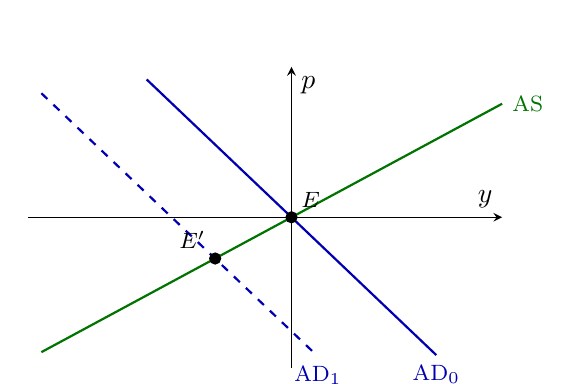
\begin{tikzpicture}
\begin{axis}[width=7.6cm,height=5.4cm,xmin=-1,xmax=0.8,ymin=-1.2,ymax=1.2,xlabel={$y$},ylabel={$p$},axis lines=middle,
  xtick=\empty,ytick=\empty,clip=false]
\addplot[green!45!black,thick,domain=-0.95:0.8] {1.133*x} node[right] {\footnotesize AS};
\addplot[blue!70!black,thick,domain=-0.55:0.55] {-2*x} node[below] {\footnotesize AD$_0$};
\addplot[blue!70!black,thick,dashed,domain=-0.95:0.1] {-2*(x+0.455)} node[below] {\footnotesize AD$_1$};
\addplot[only marks,mark=*] coordinates {(0,0) (-0.290,-0.329)};
\node[above right] at (axis cs:0,0) {\footnotesize $E$};
\node[above left] at (axis cs:-0.29,-0.329) {\footnotesize $E'$};
\end{axis}
\end{tikzpicture}
\end{center}
\passo{policy}{To restore $p=p^e$ and $y=y_n$, set $dp=dy=0$ in \eqref{b8:AD} differentiated with $di\neq0$:}
\begin{align*}
0&=d\bar y_n-\sigma\,di,\\
di&=\frac{d\bar y_n}{\sigma}\\
&=\frac{\big(-\frac{d\bar\tau}{\sigma^{-1}+\eta}\big)}{\sigma}\\
&=-\frac{d\bar\tau}{\sigma(\sigma^{-1}+\eta)}=-\frac{(1)}{0.5\times2.2}=-0.909 .
\end{align*}
Cut $i$ by $0.909$ points: AD returns to AD$_0$, so $y=y_n=y_e$ and $p=p^e$ together.
No trade-off: the shock is to demand and leaves $y_n=y_e$ (the divine coincidence, Block 9). Raising $i$ would deepen the fall.
\intuicao{Future taxes make households poorer in the long run, so they consume less now; with preset prices, output falls.}
\refbib{Benigno (2015), \S4, eq.~(13) (taxes in the markup); \S5, eqs.~(20)--(21); \S8, p.~514; Prova~01, Q3(a)--(b).}
\rubrica{\item $dy$, $dp$ and both gaps: 1.5 pts. \item Numbers: 0.5 pt. \item Graph: axes, AD shift left, AS fixed, $E'$: 1 pt.
\item Policy sign and no trade-off: 1 pt. Shifting the AS: max.\ 1 pt in the item. Raising $i$: 0 for the policy line.}
\end{sol}

% =============================================================================
% Block 9 --- Aula 9: AS-AD policy (Benigno 2015, sections 6-12). Notation: see Block 8. Checks: practice-all-topics-check-b.py, Block 9.
% Solution format (rules/00_estilo_avaliacao.md §4): Notation list, numbered equations cited with \eqref,
% one operation per displayed line. Labels: b9q<question>:<name>; AD/AS are \eqref{b8:AD}, \eqref{b8:AS}.
\bloco{9}{AS--AD policy: shocks, divine coincidence, optimal policy, multipliers, ZLB}{Benigno (2015) \S\S6--12 (Aula 9) \,\textbullet\, 25 points}

\questao{(5 points) Objective items.}

\textbf{a)} (3 points) Which shock leaves the central bank a trade-off between $p=p^e$ and $y=y_e$, and why?
\begin{alternativas}
\item A temporary rise in the current markup $\mu$: it lowers $y_n$ but not $y_e$, so $p=p^e$ and $y=y_e$ cannot both hold on the AS.
\item A temporary rise in productivity $a$: it lowers $p$ along the AD, so a cut in $i$ cannot bring $p$ back to $p^e$ without a gap.
\item News of a higher long-run markup $\bar\mu$: it shifts the AS up today and separates $y_n$ from $y_e$ in the current period.
\item News of higher long-run productivity $\bar a$: it lifts demand above $y_e$, and raising $i$ lowers $p$ but leaves a positive gap.
\end{alternativas}
\gabarito{A}
\begin{sol}
\begin{notacao}
\item $y_n$, $y_e$: natural and efficient output; $\mu$, $\bar\mu$: current and long-run markups; $a$, $\bar a$: productivity; $y_n'$: natural output after the shock.
\end{notacao}
\passo{key}{Efficient output is natural output \eqref{b8q22:yn} without the markup:}
\begin{equation}
y_e=\frac{(1+\eta)a+\sigma^{-1}g}{\sigma^{-1}+\eta}. \label{b9q25:ye}
\end{equation}
Subtracting \eqref{b9q25:ye} from \eqref{b8q22:yn}:
\begin{align}
y_n-y_e&=\Big(\frac{(1+\eta)a+\sigma^{-1}g-\mu}{\sigma^{-1}+\eta}\Big)-\Big(\frac{(1+\eta)a+\sigma^{-1}g}{\sigma^{-1}+\eta}\Big)\nonumber\\
&=-\frac{\mu}{\sigma^{-1}+\eta}, \label{b9q25:gap}
\end{align}
which depends on the current markup only. After $\mu\uparrow$ the AS \eqref{b8:AS} passes through $(y_n',p^e)$ with $y_n'<y_e$:
on it, $p=p^e$ means $y=y_n'\neq y_e$. Since $i$ moves only the AD, the bank picks a point on that AS; none gives both.
\passo{distractors}{B: by \eqref{b9q25:gap}, $a$ moves $y_n$ and $y_e$ together, so a cut in $i$ restores $p=p^e$ \emph{and} $y=y_n=y_e$ (\S6.1). C makes two mistakes:
$\bar\mu$ moves the AD, not the AS, and it leaves current $y_n=y_e$ (so the bank offsets it fully). D: raising $i$ by $d\bar y_n/\sigma$ returns
the AD to $E$, closing price and output gaps at once (\S6.3).}
\refbib{Benigno (2015), \S6--\S7, Figs.~6--9, pp.~511--514; \S11, p.~522.}
\end{sol}

\medskip
\textbf{b)} (2 points, T or F) A temporary rise in the labor-income tax $\tau$ (with $i$, $\bar p$, $p^e$ fixed) lowers output and also lowers
the output gap $y-y_n$.
\gabarito{F}
\begin{sol}
\begin{notacao}
\item $\tau$: labor-income tax (part of $\mu$); $D\equiv(\sigma^{-1}+\eta)(1+\sigma\kappa)>0$ (defined below); $\kappa>0$: AS slope.
\end{notacao}
\passo{proof}{Differentiate \eqref{b8:AD} with $\bar y_n$, $g$, $i$, $\bar p$ fixed, and \eqref{b8:AS} with $p^e$ fixed:}
\begin{equation}
dy=-\sigma\,dp,\qquad dp=\kappa(dy-dy_n). \label{b9q25:dADAS}
\end{equation}
Substitute the second equation of \eqref{b9q25:dADAS} into the first and solve for $dy$:
\begin{align}
dy&=-\sigma\big(\kappa(dy-dy_n)\big)\nonumber\\
dy&=\frac{\sigma\kappa\,dy_n}{1+\sigma\kappa}. \label{b9q25:dy}
\end{align}
By \eqref{b8q22:yn}, with $d\mu=d\tau$,
\begin{equation}
dy_n=-\frac{d\tau}{\sigma^{-1}+\eta}. \label{b9q25:dyn}
\end{equation}
Substitute \eqref{b9q25:dyn} into \eqref{b9q25:dy}, with $D\equiv(\sigma^{-1}+\eta)(1+\sigma\kappa)$:
\begin{align}
dy&=\frac{\sigma\kappa\,\big(-\frac{d\tau}{\sigma^{-1}+\eta}\big)}{1+\sigma\kappa}\nonumber\\
\frac{dy}{d\tau}&=-\frac{\kappa\sigma}{D}<0. \label{b9q25:dydtau}
\end{align}
Subtract \eqref{b9q25:dyn} from \eqref{b9q25:dydtau}, writing $\frac1{\sigma^{-1}+\eta}=\frac{1+\sigma\kappa}{D}$:
\begin{align*}
\frac{d(y-y_n)}{d\tau}&=-\frac{\kappa\sigma}{D}+\frac{1+\sigma\kappa}{D}\\
&=\frac1D>0 .
\end{align*}
The tax cuts $y_n$ by more than it cuts $y$, so the gap rises.
\refbib{Benigno (2015), \S8, eqs.~(22)--(23), Table~1, pp.~514--515.}
\end{sol}

% -----------------------------------------------------------------------------
\questao{(8 points) \textit{Source: built on Benigno, P. (2015), ``New-Keynesian Economics: An AS--AD View'', \S8, pp.~514--516
--- the article has no exercises; the statement below is ours.}
The spending multiplier: Benigno's eqs.~(22)--(23), Tables~1--2. Take $i=\rho$, $\bar p=p^e=0$, $a=\mu=0$, and a temporary rise in
$g$ with $\bar g$ fixed.}

\noindent What the article states (p.~514): ``In particular, an increase in current public expenditure, $g\uparrow$, increases output.
The increase is one-to-one in the special case of linear disutility of labor, i.e.\ $\eta=0$; otherwise the increase is less than
proportional.''

\textbf{a)} (3 points) Derive the output multiplier $m_g=dy/dg$ from the AD and AS curves. Show that $m_g\le1$, with equality iff $\eta=0$.
\resolespaco
\begin{sol}
\begin{notacao}
\item $g$, $\bar g$: government spending today and in the long run (log deviations); $m_g=dy/dg$: output multiplier.
\item $\sigma>0$, $\eta\ge0$, $\kappa>0$ as in Block 8; $D\equiv(\sigma^{-1}+\eta)(1+\sigma\kappa)$.
\end{notacao}
\passo{setup}{With $i=\rho$, $\bar p=p^e=0$ and no consumption taxes, \eqref{b8:AD} and \eqref{b8:AS} become}
\begin{align}
y&=\bar y_n+(g-\bar g)-\sigma[(\rho)-((0)-p)-(0)-\rho]\nonumber\\
y&=\bar y_n+g-\bar g-\sigma p, \label{b9q26:AD}\\
p-(0)&=\kappa(y-y_n)\nonumber\\
p&=\kappa(y-y_n), \label{b9q26:AS}
\end{align}
and \eqref{b8q22:yn} with $a=\mu=0$ gives
\begin{align}
y_n&=\frac{(1+\eta)(0)+\sigma^{-1}g-(0)}{\sigma^{-1}+\eta}\nonumber\\
&=\frac{\sigma^{-1}g}{\sigma^{-1}+\eta}. \label{b9q26:yn}
\end{align}
Substitute \eqref{b9q26:AS} into \eqref{b9q26:AD}:
\begin{align}
y&=\bar y_n+g-\bar g-\sigma\big(\kappa(y-y_n)\big)\nonumber\\
y&=\bar y_n+g-\bar g-\sigma\kappa y+\sigma\kappa y_n\nonumber\\
(1+\sigma\kappa)\,y&=g+\bar y_n-\bar g+\sigma\kappa\,y_n. \label{b9q26:comb}
\end{align}
\passo{multiplier}{In \eqref{b9q26:comb}, $g$ enters directly ($+1$) and through $y_n$; by \eqref{b9q26:yn} the second channel is
$\sigma\kappa\cdot\frac{\sigma^{-1}}{\sigma^{-1}+\eta}=\frac{\kappa}{\sigma^{-1}+\eta}$. Differentiating \eqref{b9q26:comb} with respect to $g$:}
\begin{align}
(1+\sigma\kappa)\,m_g&=1+\sigma\kappa\Big(\frac{\sigma^{-1}}{\sigma^{-1}+\eta}\Big)\nonumber\\
m_g&=\frac{1+\frac{\kappa}{\sigma^{-1}+\eta}}{1+\sigma\kappa}\nonumber\\
&=\frac{\sigma^{-1}+\eta+\kappa}{D}. \label{b9q26:mg}
\end{align}
\passo{bound}{From the first line of \eqref{b9q26:mg}:}
\begin{align*}
m_g\le1&\iff1+\frac{\kappa}{\sigma^{-1}+\eta}\le1+\sigma\kappa\\
&\iff\frac1{\sigma^{-1}+\eta}\le\sigma\\
&\iff1\le1+\sigma\eta\\
&\iff\eta\ge0 .
\end{align*}
Equivalently, since $D=\sigma^{-1}+\eta+\kappa+\sigma\kappa\eta$, the second line of \eqref{b9q26:mg} gives
\begin{align}
1-m_g&=1-\Big(\frac{\sigma^{-1}+\eta+\kappa}{D}\Big)\nonumber\\
&=\frac{(\sigma^{-1}+\eta+\kappa+\sigma\kappa\eta)-(\sigma^{-1}+\eta+\kappa)}{D}\nonumber\\
&=\frac{\sigma\kappa\eta}{D}, \label{b9q26:1mg}
\end{align}
zero iff $\eta=0$. With $\eta>0$, spending raises prices and the real rate, crowding out consumption.
\rubrica{\item AD and AS combined: 1 pt. \item $m_g$ with both channels: 1 pt. \item Bound with the iff: 1 pt.}
\end{sol}

\textbf{b)} (3 points) Find the multiplier on the gap $y-y_n$ and on the efficient gap $y-y_e$. Why are they so much smaller than $m_g$?
\resolespaco
\begin{sol}
\begin{notacao}
\item Symbols as in (a); $y_e$: efficient output \eqref{b9q25:ye}.
\end{notacao}
\passo{gap}{By \eqref{b9q26:yn}, $dy_n/dg=\frac{\sigma^{-1}}{\sigma^{-1}+\eta}$. Over the common denominator $D$,}
\begin{equation}
\frac{\sigma^{-1}}{\sigma^{-1}+\eta}=\frac{\sigma^{-1}(1+\sigma\kappa)}{D}=\frac{\sigma^{-1}+\kappa}{D}. \label{b9q26:ynD}
\end{equation}
Subtract \eqref{b9q26:ynD} from \eqref{b9q26:mg}:
\begin{align}
\frac{d(y-y_n)}{dg}&=\frac{\sigma^{-1}+\eta+\kappa-(\sigma^{-1}+\kappa)}{D}\nonumber\\
&=\frac{\eta}{D}. \label{b9q26:gapm}
\end{align}
By \eqref{b9q25:ye}, $y_e$ has the same $g$-coefficient as $y_n$ in \eqref{b8q22:yn}, so the multiplier on $y-y_e$ is also $\frac\eta D$.
\passo{why}{Most of the extra output is supply: public spending makes households poorer, so they work more and $y_n$ rises,
by \eqref{b9q26:yn} (Benigno's eq.~15). Only the part of $y$ above the new $y_n$ is a demand effect, and that is what the gap measures.}
\rubrica{\item Gap multiplier derived: 1.5 pts. \item Same for $y-y_e$, with the reason: 0.5 pt. \item Interpretation: 1 pt.}
\end{sol}

\textbf{c)} (2 points) Evaluate $\kappa$, $m_g$, the gap multiplier and $1-m_g$ at the calibration, and compare with Table~2.
\resolespaco
\begin{sol}
\begin{notacao}
\item $\alpha=0.66$: share of preset prices; $\sigma=0.5$, $\eta=0.2$, $\sigma^{-1}+\eta=2.2$ (Block 8 calibration).
\end{notacao}
\passo{numbers}{Using $\kappa=\frac{(1-\alpha)(\sigma^{-1}+\eta)}{\alpha}$, then $D$, \eqref{b9q26:mg}, \eqref{b9q26:gapm} and \eqref{b9q26:1mg}:}
\begin{align*}
\kappa&=\frac{0.34\times2.2}{0.66}=1.133,\\
1+\sigma\kappa&=1+0.5\times(1.133)\\
&=1.567,\qquad D=2.2\times1.567=3.447,\\
m_g&=\frac{2.2+1.133}{3.447}=0.967,\\
\frac{\eta}{D}&=\frac{0.2}{3.447}=0.058,\\
1-m_g&=\frac{0.5\times1.133\times0.2}{3.447}=0.033 .
\end{align*}
Table~2 prints $0.96$ for $m_g$ in this row.
\refbib{Confirmed against Benigno (2015), Table~2, p.~516, and the project's Map note on Benigno \S8 (note 07: 0.967 and 0.058).}
\rubrica{\item Each of $\kappa$, $m_g$, gap: 0.5 pt; comparison: 0.5 pt.}
\end{sol}

% -----------------------------------------------------------------------------
\questao{(12 points) Discursive. \emph{The Copom's three meetings.} Start from the efficient steady state: $y_n=y_e=0$,
$p^e=\bar p=0$, $i=\rho=2\%$. The welfare loss is $L=\frac12(y-y_e)^2+\frac{\theta}{2\kappa}(p-p^e)^2$ (eq.~33) with $\theta=8$; use the calibration of
Block~8 and work in percentage points.}

\textbf{a)} (4 points) Meeting 1: news that long-run productivity will rise, $d\bar a=1$, current $a$ unchanged (say, gains from
agricultural technology expected to last). Which curves move? Find $y$ and $p$ if the bank keeps $i=\rho$, and the optimal $i$.
Is there a trade-off? Contrast with a temporary rise in $a$.
\resolespaco
\begin{sol}
\begin{notacao}
\item $y$, $p$: output and price level; $y_n$, $y_e$: natural and efficient output; $\bar y_n$: long-run natural output; $p^e=\bar p=0$.
\item $a$, $\bar a$: current and long-run productivity; $i$: policy rate; $\rho=2\%$: rate of time preference.
\item $r_n$: natural rate of interest, the $i$ that sets $y=y_n$ at $p=p^e$ (defined in step 3); $E$: the initial equilibrium.
\item $L$: welfare loss; $\theta=8$: weight on price surprises; $\kappa=1.133$, $\sigma=0.5$, $\eta=0.2$.
\end{notacao}
\passo{curves}{Differentiate \eqref{b8q22:ybn} with respect to $\bar a$:}
\begin{align*}
d\bar y_n&=\frac{(1+\eta)\,d\bar a}{\sigma^{-1}+\eta}\\
&=\frac{(1+0.2)\times(1)}{2.2}=\frac{1.2}{2.2}=0.545 .
\end{align*}
Households expect to be richer and consume more now, so by \eqref{b8:AD} the AD shifts right by $0.545$. $y_n$ \eqref{b8q22:yn} and $y_e$
\eqref{b9q25:ye} depend on current $a$, so AS does not move.
\passo{no policy}{The algebra of Block 8, \eqref{b8q24:dy} and \eqref{b8q24:dAS}, applies with $d\bar y_n=0.545$:}
\begin{align*}
dy&=\frac{d\bar y_n}{1+\sigma\kappa}=\frac{0.545}{1.567}=0.348,\\
dp&=\kappa\,dy\\
&=1.133\times(0.348)=0.395 .
\end{align*}
Output is above both $y_n$ and $y_e$, prices above $p^e$.
\passo{policy}{With $p=\bar p$, $g=\bar g$ and no consumption taxes, \eqref{b8:AD} reads $y=\bar y_n-\sigma(i-\rho)$. Setting $y=y_n$ and solving for $i$:}
\begin{align}
(y_n)&=\bar y_n-\sigma(r_n-\rho)\nonumber\\
r_n&=\rho+\sigma^{-1}(\bar y_n-y_n). \label{b9q27:rn}
\end{align}
By \eqref{b9q27:rn}, $r_n$ rises by $0.545/0.5=1.09$ points. Setting $i=r_n$, i.e.\ \emph{raising} $i$ to $3.09\%$, returns the AD to $E$:
$y=y_n=y_e$, $p=p^e$, $L=0$. No trade-off (divine coincidence): $y_n=y_e$ throughout. A temporary $a\uparrow$ is the mirror image:
the AS shifts right, the AD stays, and the bank must \emph{cut} $i$; a permanent one needs no change.
\rubrica{\item Curve identification: 1 pt. \item No-policy equilibrium: 1 pt. \item Policy sign and size, no trade-off: 1.5 pts.
\item Contrast: 0.5 pt. Moving the AS for news, or cutting $i$: max.\ 1 pt in the item.}
\end{sol}

\textbf{b)} (5 points) Meeting 2: a temporary markup shock $\mu=5$ (say, a fuel-tax rise), $\bar\mu=0$. Find the outcome at $i=\rho$. Then
minimize $L$ subject to the AS and derive the targeting rule, $y^\ast$, $p^\ast$, and the rate $i^\ast$, comparing it with $r_n$ and $\rho$. Draw.
\resolespaco
\begin{sol}
\begin{notacao}
\item Symbols as in (a); $\mu=5$: current markup shock; $y^\ast$, $p^\ast$, $i^\ast$: optimal output, price level and rate; $E'$: no-policy point; $O$: optimum.
\end{notacao}
\passo{shock}{By \eqref{b8q22:yn} and \eqref{b9q25:ye} with $a=g=0$:}
\begin{align*}
y_n&=\frac{(1+0.2)(0)+0.5^{-1}(0)-(5)}{2.2}\\
&=-\frac{5}{2.2}=-2.273,\qquad y_e=0 .
\end{align*}
AS shifts up through $(y_n,p^e)$; AD unchanged. At $i=\rho$, with $\bar y_n=g=\bar p=p^e=0$, \eqref{b8:AD} and \eqref{b8:AS} are
\begin{equation}
y=-\sigma p,\qquad p=\kappa(y-y_n). \label{b9q27:ADAS}
\end{equation}
Substitute the second equation of \eqref{b9q27:ADAS} into the first and solve for $y$; then use the first for $p$:
\begin{align*}
y&=-\sigma\big(\kappa(y-y_n)\big)\\
y&=\frac{\sigma\kappa\,y_n}{1+\sigma\kappa}=\frac{0.567\times(-2.273)}{1.567}=-0.822,\\
p&=-y/\sigma\\
&=-(-0.822)/0.5=1.644 .
\end{align*}
Output falls and prices rise: stagflation.
\passo{why along AS}{$i$ moves only the AD, so the bank chooses \emph{which point of the AS} the economy occupies. The loss of the statement is}
\begin{equation}
L=\tfrac12(y-y_e)^2+\frac{\theta}{2\kappa}(p-p^e)^2. \label{b9q27:L}
\end{equation}
Substitute \eqref{b8:AS}, $p-p^e=\kappa(y-y_n)$, and $y_e=0$ into \eqref{b9q27:L}:
\begin{align}
L(y)&=\tfrac12\big(y-(0)\big)^2+\frac{\theta}{2\kappa}\big(\kappa(y-y_n)\big)^2\nonumber\\
&=\tfrac12y^2+\frac{\theta\kappa}2(y-y_n)^2. \label{b9q27:Ly}
\end{align}
Differentiate \eqref{b9q27:Ly} and set it to zero (the second derivative is $1+\theta\kappa>0$):
\begin{equation}
y+\theta\kappa(y-y_n)=0. \label{b9q27:foc}
\end{equation}
Since $\kappa(y-y_n)=p-p^e$ by \eqref{b8:AS}, and $y_e=0$, \eqref{b9q27:foc} is the targeting rule
\begin{align}
y+\theta\big(p-p^e\big)&=0\nonumber\\
(y-y_e)+\theta(p-p^e)&=0. \label{b9q27:IT}
\end{align}
\passo{optimum}{Solve \eqref{b9q27:foc} for $y$; then subtract $y_n$ and use \eqref{b8:AS}:}
\begin{align}
y^\ast&=\frac{\theta\kappa\,y_n}{1+\theta\kappa}\nonumber\\
&=\frac{8\times1.133\times(-2.273)}{1+8\times1.133}\nonumber\\
&=\frac{9.067}{10.067}(-2.273)=-2.047, \label{b9q27:ystar}\\
p^\ast&=\kappa(y^\ast-y_n)\nonumber\\
&=\kappa\Big(\Big(\frac{\theta\kappa\,y_n}{1+\theta\kappa}\Big)-y_n\Big)\nonumber\\
&=-\frac{\kappa y_n}{1+\theta\kappa}=\frac{1.133\times2.273}{10.067}=0.256. \label{b9q27:pstar}
\end{align}
\passo{rate}{With $\bar y_n=g=\bar p=0$, \eqref{b8:AD} reads}
\begin{equation}
y=-\sigma(i+p-\rho). \label{b9q27:ADi}
\end{equation}
Solve \eqref{b9q27:ADi} for $i$ at \eqref{b9q27:ystar}--\eqref{b9q27:pstar}:
\begin{align*}
i^\ast&=\rho-p^\ast-y^\ast/\sigma\\
&=2-(0.256)-(-2.047)/0.5\\
&=2-0.256+4.094=5.838\% .
\end{align*}
By \eqref{b9q27:rn} with $\bar y_n=0$, the natural rate is
\begin{align*}
r_n&=\rho+\sigma^{-1}\big((0)-y_n\big)\\
&=2-\frac{(-5/2.2)}{0.5}=6.545\%.
\end{align*}
So $\rho<i^\ast<r_n$: the bank tightens, accepting a deeper fall in output to keep prices close to $p^e$, but it accommodates part of
the shock. By \eqref{b9q27:ystar}--\eqref{b9q27:pstar}, as $\theta\to\infty$, $y^\ast\to y_n$ and $p^\ast\to p^e$ (strict price stability); as $\theta\to0$, $y^\ast\to y_e$.
\begin{center}
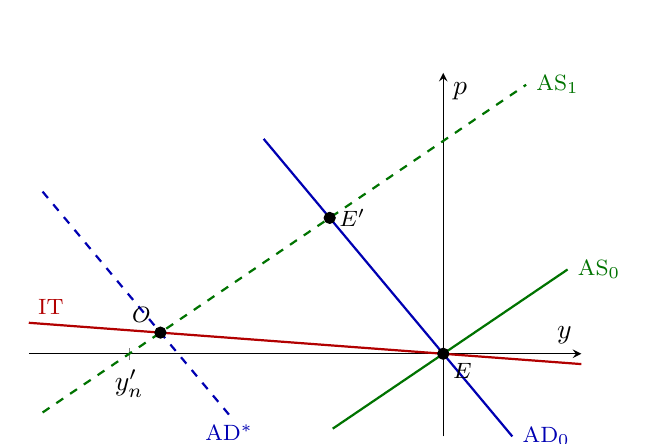
\begin{tikzpicture}
\begin{axis}[width=8.6cm,height=6.2cm,xmin=-3,xmax=1,ymin=-1,ymax=3.4,xlabel={$y$},ylabel={$p$},axis lines=middle,
  xtick={-2.273},xticklabels={$y_n'$},ytick=\empty,clip=false]
\addplot[green!45!black,thick,domain=-0.8:0.9] {1.133*x} node[right] {\footnotesize AS$_0$};
\addplot[green!45!black,thick,dashed,domain=-2.9:0.6] {1.133*(x+2.273)} node[right] {\footnotesize AS$_1$};
\addplot[blue!70!black,thick,domain=-1.3:0.5] {-2*x} node[right] {\footnotesize AD$_0$};
\addplot[blue!70!black,thick,dashed,domain=-2.9:-1.55] {0.256-2*(x+2.047)} node[below] {\footnotesize AD$^\ast$};
\addplot[red!70!black,thick,domain=-3:1] {-x/8} node[pos=0.04,above] {\footnotesize IT};
\addplot[only marks,mark=*] coordinates {(0,0) (-0.822,1.644) (-2.047,0.256)};
\node[below right] at (axis cs:0,0) {\footnotesize $E$};
\node[right] at (axis cs:-0.822,1.644) {\footnotesize $E'$};
\node[above left] at (axis cs:-2.047,0.256) {\footnotesize $O$};
\end{axis}
\end{tikzpicture}
\end{center}
\refbib{Confirmed against the Lista~7 answer in \emph{Map}, \texttt{lista-07.md}: no policy $(-0.82,+1.64)$; optimum $y^o=-2.05$, $p^o=+0.26$,
$i^o=5.84\%$ vs $r_n=6.55\%$. Benigno (2015), \S7 and \S11, eq.~(33), Fig.~14, pp.~513--514 and 521--523.}
\rubrica{\item Shock and no-policy point: 1 pt. \item Loss minimized \emph{along AS} with the reason: 1.5 pts (differentiating in $i$ with AD as the
constraint: max.\ 0.5). \item $y^\ast$, $p^\ast$, targeting rule: 1 pt. \item $i^\ast$ vs $r_n$, $\rho$, and $\theta$ limits: 0.5 pt. \item Graph with IT line and $O$: 1 pt.}
\end{sol}

\textbf{c)} (3 points) Meeting 3: news that long-run productivity will fall, $d\bar a=-5$, with $\mu=a=0$. Show that the required rate is
negative. With $i=0$, find the gap and $p$. What can the bank still do, and on what does it depend?
\resolespaco
\begin{sol}
\begin{notacao}
\item Symbols as in (a); ZLB: the zero lower bound $i\ge0$; $\bar p-p^e$: the long-run price level the bank promises, relative to preset prices.
\end{notacao}
\passo{required rate}{By \eqref{b8q22:ybn}, $\bar y_n=0.545\times(-5)=-2.727$, while $y_n=0$. By \eqref{b9q27:rn}:}
\begin{align*}
r_n&=\rho+\sigma^{-1}\big(\bar y_n-(0)\big)\\
&=2+\frac{(-2.727)}{0.5}=2-5.455=-3.455\%<0 .
\end{align*}
Cash pays zero, so $i\ge0$: the ZLB binds.
\passo{at $i=0$}{Substitute \eqref{b8:AS} into \eqref{b8:AD} (with $g=\bar g$, no consumption taxes), subtract $y_n$ and use \eqref{b9q27:rn}:}
\begin{align}
y&=\bar y_n-\sigma\big[i-\big(\bar p-(p^e+\kappa(y-y_n))\big)-\rho\big]\nonumber\\
(1+\sigma\kappa)(y-y_n)&=(\bar y_n-y_n)-\sigma\big[i-(\bar p-p^e)-\rho\big]\nonumber\\
(1+\sigma\kappa)(y-y_n)&=\big(\sigma(r_n-\rho)\big)-\sigma\big[i-(\bar p-p^e)-\rho\big]\nonumber\\
y-y_n&=\frac{\sigma}{1+\sigma\kappa}\left[r_n-i+(\bar p-p^e)\right]. \label{b9q27:gapz}
\end{align}
At $i=0$ and $\bar p=p^e$, \eqref{b9q27:gapz} and \eqref{b8:AS} give
\begin{align*}
y-y_n&=\frac{0.5}{1.567}\big[(-3.455)-(0)+(0)\big]\\
&=\frac{0.5}{1.567}(-3.455)=-1.103,\\
p-p^e&=\kappa(y-y_n)\\
&=1.133\times(-1.103)=-1.250 .
\end{align*}
\passo{expectations}{By \eqref{b9q27:gapz}, the gap closes at $i=0$ if the bank commits to a higher long-run price level,
$\bar p-p^e=-r_n=3.455$. Higher expected inflation $\bar p-p$ lowers the real rate when the nominal rate cannot fall. It works only if
the promise is credible (the bank must tolerate the higher $\bar p$ later).}
\rubrica{\item $r_n<0$: 1 pt. \item Gap and $p$ at $i=0$: 1 pt. \item The $\bar p$ commitment, its size and credibility: 1 pt.}
\end{sol}


\end{document}
